% ----------------------------------------------------------------------
%
%                            TFG.tex
%
%----------------------------------------------------------------------
%
% Este fichero contiene el "documento maestro" del documento. Lo único
% que hace es configurar el entorno LaTeX e incluir los ficheros .tex
% que contienen cada sección.
%
%----------------------------------------------------------------------
%
% Los ficheros necesarios para este documento son:
%
%       TeXiS/* : ficheros de la plantilla TeXiS.
%       Cascaras/* : ficheros con las partes del documento que no
%          son capítulos ni apéndices (portada, agradecimientos, etc.)
%       Capitulos/*.tex : capítulos de la tesis
%       Apendices/*.tex: apéndices de la tesis
%       constantes.tex: constantes LaTeX
%       config.tex : configuración de la "compilación" del documento
%       guionado.tex : palabras con guiones
%
% Para la bibliografía, además, se necesitan:
%
%       *.bib : ficheros con la información de las referencias
%
% ---------------------------------------------------------------------

\documentclass[11pt,a4paper,twoside]{book}

%
% Definimos  el   comando  \compilaCapitulo,  que   luego  se  utiliza
% (opcionalmente) en config.tex. Quedaría  mejor si también se definiera
% en  ese fichero,  pero por  el modo  en el  que funciona  eso  no es
% posible. Puedes consultar la documentación de ese fichero para tener
% más  información. Definimos también  \compilaApendice, que  tiene el
% mismo  cometido, pero  que se  utiliza para  compilar  únicamente un
% apéndice.
%
%
% Si  queremos   compilar  solo   una  parte  del   documento  podemos
% especificar mediante  \includeonly{...} qué ficheros  son los únicos
% que queremos  que se incluyan.  Esto  es útil por  ejemplo para sólo
% compilar un capítulo.
%
% El problema es que todos aquellos  ficheros que NO estén en la lista
% NO   se  incluirán...  y   eso  también   afecta  a   ficheros  de
% la plantilla...
%
% Total,  que definimos  una constante  con los  ficheros  que siempre
% vamos a querer compilar  (aquellos relacionados con configuración) y
% luego definimos \compilaCapitulo.
\newcommand{\ficherosBasicosTFG}{%
TFG/TFG_pream,TFG/TFG_cab,TFG/TFG_bib,TFG/TFG_cover%
}
\newcommand{\ficherosBasicosTexto}{%
constantes,guionado,Cascaras/bibliografia,config%
}
\newcommand{\compilaCapitulo}[1]{%
\includeonly{\ficherosBasicosTFG,\ficherosBasicosTexto,Capitulos/#1}%
}

\newcommand{\compilaApendice}[1]{%
\includeonly{\ficherosBasicosTFG,\ficherosBasicosTexto,Apendices/#1}%
}

%- - - - - - - - - - - - - - - - - - - - - - - - - - - - - - - - - - -
%            Preámbulo del documento. Configuraciones varias
%- - - - - - - - - - - - - - - - - - - - - - - - - - - - - - - - - - -

% Define  el  tipo  de  compilación que  estamos  haciendo.   Contiene
% definiciones  de  constantes que  cambian  el  comportamiento de  la
% compilación. Debe incluirse antes del paquete TeXiS/TeXiS.sty
%---------------------------------------------------------------------
%
%                          config.tex
%
%---------------------------------------------------------------------
%
% Contiene la  definición de constantes  que determinan el modo  en el
% que se compilará el documento.
%
%---------------------------------------------------------------------
%
% En concreto, podemos  indicar si queremos "modo release",  en el que
% no  aparecerán  los  comentarios  (creados  mediante  \com{Texto}  o
% \comp{Texto}) ni los "por  hacer" (creados mediante \todo{Texto}), y
% sí aparecerán los índices. El modo "debug" (o mejor dicho en modo no
% "release" muestra los índices  (construirlos lleva tiempo y son poco
% útiles  salvo  para   la  versión  final),  pero  sí   el  resto  de
% anotaciones.
%
% Si se compila con LaTeX (no  con pdflatex) en modo Debug, también se
% muestran en una esquina de cada página las entradas (en el índice de
% palabras) que referencian  a dicha página (consulta TeXiS_pream.tex,
% en la parte referente a show).
%
% El soporte para  el índice de palabras en  TeXiS es embrionario, por
% lo  que no  asumas que  esto funcionará  correctamente.  Consulta la
% documentación al respecto en TeXiS_pream.tex.
%
%
% También  aquí configuramos  si queremos  o  no que  se incluyan  los
% acrónimos  en el  documento final  en la  versión release.  Para eso
% define (o no) la constante \acronimosEnRelease.
%
% Utilizando \compilaCapitulo{nombre}  podemos también especificar qué
% capítulo(s) queremos que se compilen. Si no se pone nada, se compila
% el documento  completo.  Si se pone, por  ejemplo, 01Introduccion se
% compilará únicamente el fichero Capitulos/01Introduccion.tex
%
% Para compilar varios  capítulos, se separan sus nombres  con comas y
% no se ponen espacios de separación.
%
% En realidad  la macro \compilaCapitulo  está definida en  el fichero
% principal tesis.tex.
%
%---------------------------------------------------------------------


% Comentar la línea si no se compila en modo release.
% TeXiS hará el resto.
% ¡¡¡Si cambias esto, haz un make clean antes de recompilar!!!
\def\release{1}


% Descomentar la linea si se quieren incluir los
% acrónimos en modo release (en modo debug
% no se incluirán nunca).
% ¡¡¡Si cambias esto, haz un make clean antes de recompilar!!!
%\def\acronimosEnRelease{1}


% Descomentar la línea para establecer el capítulo que queremos
% compilar

% \compilaCapitulo{01Introduccion}
% \compilaCapitulo{02EstructuraYGeneracion}
% \compilaCapitulo{03Edicion}
% \compilaCapitulo{04Imagenes}
% \compilaCapitulo{05Bibliografia}
% \compilaCapitulo{06Makefile}

% \compilaApendice{01AsiSeHizo}

% Variable local para emacs, para  que encuentre el fichero maestro de
% compilación y funcionen mejor algunas teclas rápidas de AucTeX
%%%
%%% Local Variables:
%%% mode: latex
%%% TeX-master: "./Tesis.tex"
%%% End:


% Paquete de la plantilla
\usepackage{TeXiS/TeXiS}
\usepackage{float}
\usepackage{listings}
\usepackage{subfigure}
\usepackage{subcaption}
\usepackage{cleveref}
\usepackage{graphicx}
\usepackage{xcolor}
\usepackage[utf8]{inputenc}
\usepackage{hyperref}


\lstset{escapeinside=||}

\colorlet{punct}{red!60!black}
\definecolor{background}{HTML}{EEEEEE}
\definecolor{delim}{RGB}{20,105,176}
\colorlet{numb}{magenta!60!black}
\lstdefinelanguage{json}{
	basicstyle=\normalfont\ttfamily,
	numbers=left,
	numberstyle=\scriptsize,
	stepnumber=1,
	numbersep=8pt,
	showstringspaces=false,
	breaklines=true,
	frame=lines,
	backgroundcolor=\color{background},
	literate=
	*{0}{{{\color{numb}0}}}{1}
	{1}{{{\color{numb}1}}}{1}
	{2}{{{\color{numb}2}}}{1}
	{3}{{{\color{numb}3}}}{1}
	{4}{{{\color{numb}4}}}{1}
	{5}{{{\color{numb}5}}}{1}
	{6}{{{\color{numb}6}}}{1}
	{7}{{{\color{numb}7}}}{1}
	{8}{{{\color{numb}8}}}{1}
	{9}{{{\color{numb}9}}}{1}
	{:}{{{\color{punct}{:}}}}{1}
	{,}{{{\color{punct}{,}}}}{1}
	{\{}{{{\color{delim}{\{}}}}{1}
	{\}}{{{\color{delim}{\}}}}}{1}
	{[}{{{\color{delim}{[}}}}{1}
	{]}{{{\color{delim}{]}}}}{1},
}
\lstdefinelanguage{python}{
	basicstyle=\normalfont\ttfamily,
	numbers=left,
	numberstyle=\scriptsize,
	stepnumber=1,
	numbersep=8pt,
	showstringspaces=false,
	breaklines=true,
	frame=lines,
	backgroundcolor=\color{background},
	literate=
	*{0}{{{\color{numb}0}}}{1}
	{1}{{{\color{numb}1}}}{1}
	{2}{{{\color{numb}2}}}{1}
	{3}{{{\color{numb}3}}}{1}
	{4}{{{\color{numb}4}}}{1}
	{5}{{{\color{numb}5}}}{1}
	{6}{{{\color{numb}6}}}{1}
	{7}{{{\color{numb}7}}}{1}
	{8}{{{\color{numb}8}}}{1}
	{9}{{{\color{numb}9}}}{1}
	{:}{{{\color{punct}{:}}}}{1}
	{,}{{{\color{punct}{,}}}}{1}
	{\{}{{{\color{delim}{\{}}}}{1}
	{\}}{{{\color{delim}{\}}}}}{1}
	{[}{{{\color{delim}{[}}}}{1}
	{]}{{{\color{delim}{]}}}}{1},
}



% Incluimos el fichero con comandos de constantes
%---------------------------------------------------------------------
%
%                          constantes.tex
%
%---------------------------------------------------------------------
%
% Fichero que  declara nuevos comandos LaTeX  sencillos realizados por
% comodidad en la escritura de determinadas palabras
%
%---------------------------------------------------------------------

%%%%%%%%%%%%%%%%%%%%%%%%%%%%%%%%%%%%%%%%%%%%%%%%%%%%%%%%%%%%%%%%%%%%%%
% Comando: 
%
%       \titulo
%
% Resultado: 
%
% Escribe el título del documento.
%%%%%%%%%%%%%%%%%%%%%%%%%%%%%%%%%%%%%%%%%%%%%%%%%%%%%%%%%%%%%%%%%%%%%%
\def\titulo{\textsc{TeXiS}: Una plantilla de \LaTeX\
  para Tesis y otros documentos}

%%%%%%%%%%%%%%%%%%%%%%%%%%%%%%%%%%%%%%%%%%%%%%%%%%%%%%%%%%%%%%%%%%%%%%
% Comando: 
%
%       \autor
%
% Resultado: 
%
% Escribe el autor del documento.
%%%%%%%%%%%%%%%%%%%%%%%%%%%%%%%%%%%%%%%%%%%%%%%%%%%%%%%%%%%%%%%%%%%%%%
\def\autor{Marco Antonio y Pedro Pablo G\'omez Mart\'in}

% Variable local para emacs, para  que encuentre el fichero maestro de
% compilación y funcionen mejor algunas teclas rápidas de AucTeX

%%%
%%% Local Variables:
%%% mode: latex
%%% TeX-master: "tesis.tex"
%%% End:


% Sacamos en el log de la compilación el copyright
%\typeout{Copyright Marco Antonio and Pedro Pablo Gomez Martin}

%
% "Metadatos" para el PDF
%
\ifpdf\hypersetup{%
    pdftitle = {\titulo},
    pdfsubject = {Plantilla de Tesis},
    pdfkeywords = {Plantilla, LaTeX, tesis, trabajo de
      investigación, trabajo de Master},
    pdfauthor = {\textcopyright\ \autor},
    pdfcreator = {\LaTeX\ con el paquete \flqq hyperref\frqq},
    pdfproducer = {pdfeTeX-0.\the\pdftexversion\pdftexrevision},
    }
    \pdfinfo{/CreationDate (\today)}
\fi


%- - - - - - - - - - - - - - - - - - - - - - - - - - - - - - - - - - -
%                        Documento
%- - - - - - - - - - - - - - - - - - - - - - - - - - - - - - - - - - -
\begin{document}
	
	% Incluimos el  fichero de definición de guionado  de algunas palabras
	% que LaTeX no ha dividido como debería
	%----------------------------------------------------------------
%
%                          guionado.tex
%
%----------------------------------------------------------------
%
% Fichero con algunas divisiones de palabras que LaTeX no
% hace correctamente si no se le da alguna ayuda.
%
%----------------------------------------------------------------

\hyphenation{
% a
abs-trac-to
abs-trac-tos
abs-trac-ta
abs-trac-tas
ac-tua-do-res
a-gra-de-ci-mien-tos
ana-li-za-dor
an-te-rio-res
an-te-rior-men-te
apa-rien-cia
a-pro-pia-do
a-pro-pia-dos
a-pro-pia-da
a-pro-pia-das
a-pro-ve-cha-mien-to
a-que-llo
a-que-llos
a-que-lla
a-que-llas
a-sig-na-tu-ra
a-sig-na-tu-ras
a-so-cia-da
a-so-cia-das
a-so-cia-do
a-so-cia-dos
au-to-ma-ti-za-do
% b
batch
bi-blio-gra-fía
bi-blio-grá-fi-cas
bien
bo-rra-dor
boo-l-ean-expr
% c
ca-be-ce-ra
call-me-thod-ins-truc-tion
cas-te-lla-no
cir-cuns-tan-cia
cir-cuns-tan-cias
co-he-ren-te
co-he-ren-tes
co-he-ren-cia
co-li-bri
co-men-ta-rio
co-mer-cia-les
co-no-ci-mien-to
cons-cien-te
con-si-de-ra-ba
con-si-de-ra-mos
con-si-de-rar-se
cons-tan-te
cons-trucción
cons-tru-ye
cons-tru-ir-se
con-tro-le
co-rrec-ta-men-te
co-rres-pon-den
co-rres-pon-dien-te
co-rres-pon-dien-tes
co-ti-dia-na
co-ti-dia-no
crean
cris-ta-li-zan
cu-rri-cu-la
cu-rri-cu-lum
cu-rri-cu-lar
cu-rri-cu-la-res
% d
de-di-ca-do
de-di-ca-dos
de-di-ca-da
de-di-ca-das
de-rro-te-ro
de-rro-te-ros
de-sa-rro-llo
de-sa-rro-llos
de-sa-rro-lla-do
de-sa-rro-lla-dos
de-sa-rro-lla-da
de-sa-rro-lla-das
de-sa-rro-lla-dor
de-sa-rro-llar
des-cri-bi-re-mos
des-crip-ción
des-crip-cio-nes
des-cri-to
des-pués
de-ta-lla-do
de-ta-lla-dos
de-ta-lla-da
de-ta-lla-das
di-a-gra-ma
di-a-gra-mas
di-se-ños
dis-po-ner
dis-po-ni-bi-li-dad
do-cu-men-ta-da
do-cu-men-to
do-cu-men-tos
% e
edi-ta-do
e-du-ca-ti-vo
e-du-ca-ti-vos
e-du-ca-ti-va
e-du-ca-ti-vas
e-la-bo-ra-do
e-la-bo-ra-dos
e-la-bo-ra-da
e-la-bo-ra-das
es-co-llo
es-co-llos
es-tu-dia-do
es-tu-dia-dos
es-tu-dia-da
es-tu-dia-das
es-tu-dian-te
e-va-lua-cio-nes
e-va-lua-do-res
exis-ten-tes
exhaus-ti-va
ex-pe-rien-cia
ex-pe-rien-cias
% f
for-ma-li-za-do
% g
ge-ne-ra-ción
ge-ne-ra-dor
ge-ne-ra-do-res
ge-ne-ran
% h
he-rra-mien-ta
he-rra-mien-tas
% i
i-dio-ma
i-dio-mas
im-pres-cin-di-ble
im-pres-cin-di-bles
in-de-xa-do
in-de-xa-dos
in-de-xa-da
in-de-xa-das
in-di-vi-dual
in-fe-ren-cia
in-fe-ren-cias
in-for-ma-ti-ca
in-gre-dien-te
in-gre-dien-tes
in-me-dia-ta-men-te
ins-ta-la-do
ins-tan-cias
% j
% k
% l
len-gua-je
li-be-ra-to-rio
li-be-ra-to-rios
li-be-ra-to-ria
li-be-ra-to-rias
li-mi-ta-do
li-te-ra-rio
li-te-ra-rios
li-te-ra-ria
li-te-ra-rias
lo-tes
% m
ma-ne-ra
ma-nual
mas-que-ra-de
ma-yor
me-mo-ria
mi-nis-te-rio
mi-nis-te-rios
mo-de-lo
mo-de-los
mo-de-la-do
mo-du-la-ri-dad
mo-vi-mien-to
% n
na-tu-ral
ni-vel
nues-tro
% o
obs-tan-te
o-rien-ta-do
o-rien-ta-dos
o-rien-ta-da
o-rien-ta-das
% p
pa-ra-le-lo
pa-ra-le-la
par-ti-cu-lar
par-ti-cu-lar-men-te
pe-da-gó-gi-ca
pe-da-gó-gi-cas
pe-da-gó-gi-co
pe-da-gó-gi-cos
pe-rio-di-ci-dad
per-so-na-je
plan-te-a-mien-to
plan-te-a-mien-tos
po-si-ción
pre-fe-ren-cia
pre-fe-ren-cias
pres-cin-di-ble
pres-cin-di-bles
pri-me-ra
pro-ble-ma
pro-ble-mas
pró-xi-mo
pu-bli-ca-cio-nes
pu-bli-ca-do
% q
% r
rá-pi-da
rá-pi-do
ra-zo-na-mien-to
ra-zo-na-mien-tos
re-a-li-zan-do
re-fe-ren-cia
re-fe-ren-cias
re-fe-ren-cia-da
re-fe-ren-cian
re-le-van-tes
re-pre-sen-ta-do
re-pre-sen-ta-dos
re-pre-sen-ta-da
re-pre-sen-ta-das
re-pre-sen-tar-lo
re-qui-si-to
re-qui-si-tos
res-pon-der
res-pon-sa-ble
% s
se-pa-ra-do
si-guien-do
si-guien-te
si-guien-tes
si-guie-ron
si-mi-lar
si-mi-la-res
si-tua-ción
% t
tem-pe-ra-ments
te-ner
trans-fe-ren-cia
trans-fe-ren-cias
% u
u-sua-rio
Unreal-Ed
% v
va-lor
va-lo-res
va-rian-te
ver-da-de-ro
ver-da-de-ros
ver-da-de-ra
ver-da-de-ras
ver-da-de-ra-men-te
ve-ri-fi-ca
% w
% x
% y
% z
}
% Variable local para emacs, para que encuentre el fichero
% maestro de compilación
%%%
%%% Local Variables:
%%% mode: latex
%%% TeX-master: "./Tesis.tex"
%%% End:

	
	% Marcamos  el inicio  del  documento para  la  numeración de  páginas
	% (usando números romanos para esta primera fase).
	\frontmatter
	\pagestyle{empty}
	
	%---------------------------------------------------------------------
%
%                          configCover.tex
%
%---------------------------------------------------------------------
%
% cover.tex
% Copyright 2009 Marco Antonio Gomez-Martin, Pedro Pablo Gomez-Martin
%
% This file belongs to the TeXiS manual, a LaTeX template for writting
% Thesis and other documents. The complete last TeXiS package can
% be obtained from http://gaia.fdi.ucm.es/projects/texis/
%
% Although the TeXiS template itself is distributed under the 
% conditions of the LaTeX Project Public License
% (http://www.latex-project.org/lppl.txt), the manual content
% uses the CC-BY-SA license that stays that you are free:
%
%    - to share & to copy, distribute and transmit the work
%    - to remix and to adapt the work
%
% under the following conditions:
%
%    - Attribution: you must attribute the work in the manner
%      specified by the author or licensor (but not in any way that
%      suggests that they endorse you or your use of the work).
%    - Share Alike: if you alter, transform, or build upon this
%      work, you may distribute the resulting work only under the
%      same, similar or a compatible license.
%
% The complete license is available in
% http://creativecommons.org/licenses/by-sa/3.0/legalcode
%
%---------------------------------------------------------------------
%
% Fichero que contiene la configuración de la portada y de la 
% primera hoja del documento.
%
%---------------------------------------------------------------------


% Pueden configurarse todos los elementos del contenido de la portada
% utilizando comandos.

%%%%%%%%%%%%%%%%%%%%%%%%%%%%%%%%%%%%%%%%%%%%%%%%%%%%%%%%%%%%%%%%%%%%%%
% Título del documento:
% \tituloPortada{titulo}
% Nota:
% Si no se define se utiliza el del \titulo. Este comando permite
% cambiar el título de forma que se especifiquen dónde se quieren
% los retornos de carro cuando se utilizan fuentes grandes.
%%%%%%%%%%%%%%%%%%%%%%%%%%%%%%%%%%%%%%%%%%%%%%%%%%%%%%%%%%%%%%%%%%%%%%
\tituloPortada{%
Asistente web interactivo para la simplificación de textos
}

%%%%%%%%%%%%%%%%%%%%%%%%%%%%%%%%%%%%%%%%%%%%%%%%%%%%%%%%%%%%%%%%%%%%%%
% Autor del documento:
% \autorPortada{Nombre}
% Se utiliza en la portada y en el valor por defecto del
% primer subtítulo de la segunda portada.
%%%%%%%%%%%%%%%%%%%%%%%%%%%%%%%%%%%%%%%%%%%%%%%%%%%%%%%%%%%%%%%%%%%%%%
\autorPortada{Javier Sesé García \\ Estefanía Ortega Ávila}

%%%%%%%%%%%%%%%%%%%%%%%%%%%%%%%%%%%%%%%%%%%%%%%%%%%%%%%%%%%%%%%%%%%%%%
% Fecha de publicación:
% \fechaPublicacion{Fecha}
% Puede ser vacío. Aparece en la última línea de ambas portadas
%%%%%%%%%%%%%%%%%%%%%%%%%%%%%%%%%%%%%%%%%%%%%%%%%%%%%%%%%%%%%%%%%%%%%%
\fechaPublicacion{\today}

%%%%%%%%%%%%%%%%%%%%%%%%%%%%%%%%%%%%%%%%%%%%%%%%%%%%%%%%%%%%%%%%%%%%%%
% Imagen de la portada (y escala)
% \imagenPortada{Fichero}
% \escalaImagenPortada{Numero}
% Si no se especifica, se utiliza la imagen TODO.pdf
%%%%%%%%%%%%%%%%%%%%%%%%%%%%%%%%%%%%%%%%%%%%%%%%%%%%%%%%%%%%%%%%%%%%%%
\imagenPortada{Imagenes/Vectorial/escudoUCM}
\escalaImagenPortada{.2}

%%%%%%%%%%%%%%%%%%%%%%%%%%%%%%%%%%%%%%%%%%%%%%%%%%%%%%%%%%%%%%%%%%%%%%
% Tipo de documento.
% \tipoDocumento{Tipo}
% Para el texto justo debajo del escudo.
% Si no se indica, se utiliza "TESIS DOCTORAL".
%%%%%%%%%%%%%%%%%%%%%%%%%%%%%%%%%%%%%%%%%%%%%%%%%%%%%%%%%%%%%%%%%%%%%%
\tipoDocumento{Trabajo de Fin de Grado}

%%%%%%%%%%%%%%%%%%%%%%%%%%%%%%%%%%%%%%%%%%%%%%%%%%%%%%%%%%%%%%%%%%%%%%
% Institución/departamento asociado al documento.
% \institucion{Nombre}
% Puede tener varias líneas. Se utiliza en las dos portadas.
% Si no se indica aparecerá vacío.
%%%%%%%%%%%%%%%%%%%%%%%%%%%%%%%%%%%%%%%%%%%%%%%%%%%%%%%%%%%%%%%%%%%%%%
\institucion{%
Ingeniería Informática de Computadores\\[0.2em]
Facultad de Informática\\[0.2em]
Universidad Complutense de Madrid
}

%%%%%%%%%%%%%%%%%%%%%%%%%%%%%%%%%%%%%%%%%%%%%%%%%%%%%%%%%%%%%%%%%%%%%%
% Director del trabajo.
% \directorPortada{Nombre}
% Se utiliza para el valor por defecto del segundo subtítulo, donde
% se indica quién es el director del trabajo.
% Si se fuerza un subtítulo distinto, no hace falta definirlo.
%%%%%%%%%%%%%%%%%%%%%%%%%%%%%%%%%%%%%%%%%%%%%%%%%%%%%%%%%%%%%%%%%%%%%%
\directorPortada{Raquel Hervás Ballesteros\\ Susana Bautista Blasco}

%%%%%%%%%%%%%%%%%%%%%%%%%%%%%%%%%%%%%%%%%%%%%%%%%%%%%%%%%%%%%%%%%%%%%%
% Texto del primer subtítulo de la segunda portada.
% \textoPrimerSubtituloPortada{Texto}
% Para configurar el primer "texto libre" de la segunda portada.
% Si no se especifica se indica "Memoria que presenta para optar al
% título de Doctor en Informática" seguido del \autorPortada.
%%%%%%%%%%%%%%%%%%%%%%%%%%%%%%%%%%%%%%%%%%%%%%%%%%%%%%%%%%%%%%%%%%%%%%
\textoPrimerSubtituloPortada{%
\textbf{Trabajo de Fin de Grado en Ingeniería Informática}  \\ [0.3em]
\textbf{Departamento de XXXXXXXXXXXXX} \\ [0.3em]
}

%%%%%%%%%%%%%%%%%%%%%%%%%%%%%%%%%%%%%%%%%%%%%%%%%%%%%%%%%%%%%%%%%%%%%%
% Texto del segundo subtítulo de la segunda portada.
% \textoSegundoSubtituloPortada{Texto}
% Para configurar el segundo "texto libre" de la segunda portada.
% Si no se especifica se indica "Dirigida por el Doctor" seguido
% del \directorPortada.
%%%%%%%%%%%%%%%%%%%%%%%%%%%%%%%%%%%%%%%%%%%%%%%%%%%%%%%%%%%%%%%%%%%%%%
\textoSegundoSubtituloPortada{%
\textbf{Convocatoria: }\textit{Febrero/Junio/Septiembre \the\year} \\ [0.2em]
\textbf{Calificación: }\textit{Nota}
}

%%%%%%%%%%%%%%%%%%%%%%%%%%%%%%%%%%%%%%%%%%%%%%%%%%%%%%%%%%%%%%%%%%%%%%
% \explicacionDobleCara
% Si se utiliza, se aclara que el documento está preparado para la
% impresión a doble cara.
%%%%%%%%%%%%%%%%%%%%%%%%%%%%%%%%%%%%%%%%%%%%%%%%%%%%%%%%%%%%%%%%%%%%%%
\explicacionDobleCara

%%%%%%%%%%%%%%%%%%%%%%%%%%%%%%%%%%%%%%%%%%%%%%%%%%%%%%%%%%%%%%%%%%%%%%
% \isbn
% Si se utiliza, aparecerá el ISBN detrás de la segunda portada.
%%%%%%%%%%%%%%%%%%%%%%%%%%%%%%%%%%%%%%%%%%%%%%%%%%%%%%%%%%%%%%%%%%%%%%
%\isbn{978-84-692-7109-4}


%%%%%%%%%%%%%%%%%%%%%%%%%%%%%%%%%%%%%%%%%%%%%%%%%%%%%%%%%%%%%%%%%%%%%%
% \copyrightInfo
% Si se utiliza, aparecerá información de los derechos de copyright
% detrás de la segunda portada.
%%%%%%%%%%%%%%%%%%%%%%%%%%%%%%%%%%%%%%%%%%%%%%%%%%%%%%%%%%%%%%%%%%%%%%
\copyrightInfo{\autor}


%%
%% Creamos las portadas
%%
\makeCover

% Variable local para emacs, para que encuentre el fichero
% maestro de compilación
%%%
%%% Local Variables:
%%% mode: latex
%%% TeX-master: "../Tesis.tex"
%%% End:

	\chapter*{Autorización de difusión}

   
El abajo firmante, matriculado en el Máster en Ingeniería en Informática de la Facultad de Informática, autoriza a la Universidad Complutense de Madrid (UCM) a difundir y utilizar con fines académicos, no comerciales y mencionando expresamente a su autor el presente Trabajo Fin de Máster: ``TITULO DEL TRABAJO'', realizado durante el curso académico CURSO bajo la dirección de DIRECTORES en el Departamento de XXXXXXXXXXXXXXXXXXXXXXXX, y a la Biblioteca de la UCM a depositarlo en el Archivo Institucional E-Prints Complutense con el objeto de incrementar la difusión, uso e impacto del trabajo en Internet y garantizar su preservación y acceso a largo plazo.

\vspace{5cm}

% +--------------------------------------------------------------------+
% | On the line below, replace "Enter Your Name" with your name
% | Use the same form of your name as it appears on your title page.
% | Use mixed case, for example, Lori Goetsch.
% +--------------------------------------------------------------------+
\begin{center}
	\large Nombre Del Alumno\\
	
	\vspace{0.5cm}
	
	% +--------------------------------------------------------------------+
	% | On the line below, replace Fecha
	% |
	% +--------------------------------------------------------------------+
	
	\today\\
	
\end{center}

	% +--------------------------------------------------------------------+
% | Dedication Page (Optional)
% +--------------------------------------------------------------------+

\chapter*{Dedicatoria}


Texto de la dedicatoria...
	% +--------------------------------------------------------------------+
% | Acknowledgements Page (Optional)                                   |
% +--------------------------------------------------------------------+

\chapter*{Agradecimientos}

Texto de los agradecimientos












	\chapter*{Resumen}

Resumen en español del trabajo


\section*{Palabras clave}
   
\noindent Máximo 10 palabras clave separadas por comas

   



	\begin{otherlanguage}{english}
		\chapter*{Abstract}

Abstract in English.


\section*{Keywords}

\noindent 10 keywords max., separated by commas.




		% Si el trabajo se escribe en inglés, comentar esta línea y descomentar
		% otra igual que hay justo antes de \end{document}
	\end{otherlanguage}
	
	\ifx\generatoc\undefined
	\else
	%---------------------------------------------------------------------
%
%                          TeXiS_toc.tex
%
%---------------------------------------------------------------------
%
% TeXiS_toc.tex
% Copyright 2009 Marco Antonio Gomez-Martin, Pedro Pablo Gomez-Martin
%
% This file belongs to TeXiS, a LaTeX template for writting
% Thesis and other documents. The complete last TeXiS package can
% be obtained from http://gaia.fdi.ucm.es/projects/texis/
%
% This work may be distributed and/or modified under the
% conditions of the LaTeX Project Public License, either version 1.3
% of this license or (at your option) any later version.
% The latest version of this license is in
%   http://www.latex-project.org/lppl.txt
% and version 1.3 or later is part of all distributions of LaTeX
% version 2005/12/01 or later.
%
% This work has the LPPL maintenance status `maintained'.
% 
% The Current Maintainers of this work are Marco Antonio Gomez-Martin
% and Pedro Pablo Gomez-Martin
%
%---------------------------------------------------------------------
%
% Contiene  los  comandos  para  generar los  índices  del  documento,
% entendiendo por índices las tablas de contenidos.
%
% Genera  el  índice normal  ("tabla  de  contenidos"),  el índice  de
% figuras y el de tablas. También  crea "marcadores" en el caso de que
% se esté compilando con pdflatex para que aparezcan en el PDF.
%
%---------------------------------------------------------------------


% Primero un poquito de configuración...


% Pedimos que inserte todos los epígrafes hasta el nivel \subsection en
% la tabla de contenidos.
\setcounter{tocdepth}{2} 

% Le  pedimos  que nos  numere  todos  los  epígrafes hasta  el  nivel
% \subsubsection en el cuerpo del documento.
\setcounter{secnumdepth}{3} 


% Creamos los diferentes índices.

% Lo primero un  poco de trabajo en los marcadores  del PDF. No quiero
% que  salga una  entrada  por cada  índice  a nivel  0...  si no  que
% aparezca un marcador "Índices", que  tenga dentro los otros tipos de
% índices.  Total, que creamos el marcador "Índices".
% Antes de  la creación  de los índices,  se añaden los  marcadores de
% nivel 1.

\ifpdf
   \pdfbookmark{Índices}{indices}
\fi

% Tabla de contenidos.
%
% La  inclusión  de '\tableofcontents'  significa  que  en la  primera
% pasada  de  LaTeX  se  crea   un  fichero  con  extensión  .toc  con
% información sobre la tabla de contenidos (es conceptualmente similar
% al  .bbl de  BibTeX, creo).  En la  segunda ejecución  de  LaTeX ese
% documento se utiliza para  generar la verdadera página de contenidos
% usando la  información sobre los  capítulos y demás guardadas  en el
% .toc
\ifpdf
   \pdfbookmark[1]{Tabla de Contenidos}{tabla de contenidos}
\fi

\cabeceraEspecial{\'Indice}

\tableofcontents

\newpage 

% Índice de figuras
%
% La idea es semejante que para  el .toc del índice, pero ahora se usa
% extensión .lof (List Of Figures) con la información de las figuras.

\ifpdf
   \pdfbookmark[1]{Índice de figuras}{indice de figuras}
\fi

\cabeceraEspecial{\'Indice de figuras}

\listoffigures

\newpage

% Índice de tablas
% Como antes, pero ahora .lot (List Of Tables)

\ifpdf
   \pdfbookmark[1]{Índice de tablas}{indice de tablas}
\fi

\cabeceraEspecial{\'Indice de tablas}

\listoftables

\newpage

% Variable local para emacs, para  que encuentre el fichero maestro de
% compilación y funcionen mejor algunas teclas rápidas de AucTeX

%%%
%%% Local Variables:
%%% mode: latex
%%% TeX-master: "../Tesis.tex"
%%% End:

	\fi
	
	% Marcamos el  comienzo de  los capítulos (para  la numeración  de las
	% páginas) y ponemos la cabecera normal
	\mainmatter
	
	\pagestyle{fancy}
	\restauraCabecera
	
	%%%%%%%%%%%%%%%%%%%%%%%%%%%%%%%%%%%%%%%%%%%%%%%%%%%%%%%%%%%%%%%%%%%%%%%%%%%
	% Si el TFM se escribe en ingles, comentar las siguientes líneas 
	% porque no hace falta incluir nuevamente la Introducción en inglés
	\begin{otherlanguage}{english}
		\chapter{Introduction}
\label{cap:introduction}

Introduction to the subject area.










	\end{otherlanguage}
	\addtocounter{chapter}{-1} 
	%%%%%%%%%%%%%%%%%%%%%%%%%%%%%%%%%%%%%%%%%%%%%%%%%%%%%%%%%%%%%%%%%%%%%%%%%%%
	
	\chapter{Introducción}
\label{cap:introduccion}

\chapterquote{Frase célebre dicha por alguien inteligente}{Autor}

\section{Motivación}
Introducción al tema del TFM.

\subsection{Explicaciones adicionales}
Si quieres cambiar el \textbf{estilo del título} de los capítulos, abre el fichero \verb|TeXiS\TeXiS_pream.tex| y comenta la línea \verb|\usepackage[Lenny]{fncychap}| para dejar el estilo básico de \LaTeX.

Si no te gusta que no haya \textbf{espacios entre párrafos} y quieres dejar un pequeño espacio en blanco, no metas saltos de línea (\verb|\\|) al final de los párrafos. En su lugar, busca el comando  \verb|\setlength{\parskip}{0.2ex}| en \verb|TeXiS\TeXiS_pream.tex| y aumenta el valor de $0.2ex$ a, por ejemplo, $1ex$.

El siguiente texto se genera con el comando \verb|\lipsum[2-20]| que viene a continuación en el fichero .tex. El único propósito es mostrar el aspecto de las páginas usando esta plantilla. Quita este comando y, si quieres, comenta o elimina el paquete \textit{lipsum} al final de \verb|TeXiS\TeXiS_pream.tex|

\subsubsection{Texto de prueba}


\lipsum[2-20]
	\chapter{Estado del arte}
\label{cap:estadoDeLaCuestion}


\section{¿Que es la lectura fácil?}
La lectura fácil es una forma de adaptar textos para una comprensión más sencilla del original. No se trata sólo de un resumen, sino de una simplificación del texto con un lenguaje, vocabulario, términos, oraciones, imágenes descriptivas y formato de forma simple, sencilla y adecuada para aquellas personas con discapacidad intelectual, con dificultad para el lenguaje, con alguna enfermedad y/o trastorno mental, en proceso de aprendizaje, etc. que, según estudios de la Unión Europea, alcanza al 30\% de la población.

\section{Un poco de Historia...}
El movimiento de la Lectura Fácil surgió en Suecia en 1968. En ese año se publicó el primer libro en Lectura Fácil y desde entonces hasta 1994 crearon 330 obras en lectura fácil, entre 15 y 20 nuevas cada año.

Esto se extendió a los países vecinos de Noruega y Finlandia.

En Noruega, por ejemplo, la iniciativa se denomina \textit{“Leser s$\emptyset$ker bok”} (Lector busca libro) y es una alianza de 20 organizaciones, que incluyen editoriales y organizaciones de personas con discapacidad.

En 1988 se creó en Bruselas la organización \textit{Inclusion Europe}, la alianza europea de organizaciones que trabajan por los derechos de las personas con discapacidad, que actualmente agrupa a organizaciones y asociaciones de personas con discapacidad intelectual de 40 países europeos e Israel.

En 1998 se elaboró la guía \textit{«El camino más fácil: Directrices europeas para generar información de fácil lectura destinada a personas con discapacidad intelectual»} y se diseñó un logotipo europeo de lectura fácil, para identificar todos los textos redactados que siguieran sus pautas.

En España fue en 2003 cuando se creó la primera Asociación de Lectura Fácil en Barcelona. Desde entonces, surgen diversas organizaciones e iniciativas en pro de la lectura fácil por toda España.

\section{¿Cómo se identifican los textos de lectura fácil?}
En los textos adaptados a Lectura fácil vienen determinados por dos tipos de logotipos. En la figura \ref{fig:IFLA} es el logo que la Asociación de Lectura Fácil otorga a los textos que se adaptan a las normas de la IFLA. Y la figura  \ref{fig:logoEuropeo}
Logo fomentado por Inclusion Europe.
\begin{figure}[htb]
\centering
	
\includegraphics[width=0.5\textwidth]{Imagenes/Logos/indice}
	\caption{Logo LF que cumplen las normas de la IFLA}
	\label{fig:IFLA}
\end{figure} 
\begin{figure}[htb]
	\centering
	
\includegraphics[width=0.3\textwidth]{Imagenes/Logos/indice2}
	\caption{Logotipo europeo de LF}
	\label{fig:logoEuropeo}
\end{figure} 
\section{Niveles de adaptación}
Es imposible adaptar un texto para todas las personas que necesiten este tipo de lectura.
 
La IFLA (Federación Internacional de Asociaciones de Bibliotecarios y Bibliotecas) distingue entre los siguientes niveles de adaptación:
\begin{itemize}
	\item Primer nivel, es el más sencillo y simple con muchas imágenes y escaso texto, con una dificultas sintáctica baja.
\item Segundo nivel, es intermedio, menos sencillo que el anterior con un vocabulario y expresiones que son conocidas por todos, fácil de seguir y comprender e imágenes.
\item Tercer nivel, es el más complejo, con textos largos, palabras que no se conocen a menudo, con saltos en el tiempo y muy pocas imágenes. 
 \end{itemize}
\section{Pautas a seguir para la elaboración de lectura fácil}
 El primero documento de como elaborar texto adaptado a lectura fácil fue publicado por la IFLA. Hay otro que fue elaborado por varias organizaciones de Inclusion Europe bajo el título "Información para todos". 
 
 Las pautas que se deben seguir se vincula a la ortografía, gramática, léxico, estilo, diseño, imágenes, formato, etc. 
 
 Algunos ejemplos y recomendaciones son las siguientes:
 \begin{itemize}
 \item Uso de frases simples, cortas y con una estructura habitual.
 \item Uso de imágenes sencillas y pictogramas de apoyo al texto, de manera descriptiva.
 \item Cada frase debe ocupar una línea. Si no es fuese posible deberá ocupar varias líneas.
 \item Evitar oraciones impersonales y pasivas reflejas.
 \item Evitar el subjuntivo o la voz pasiva.
 \item Evitar signos ortográficos poco habituales. (%, &, / ...)
 \item Evitar abreviaturas, acrónimos y siglas
 \item Uso de palabras de uso cotidiano y evitar tecnicismos.
 \item Ideas principales
 \item Redactar en modo directo
 \item No dar conocimientos previos por conocidos.
 \item Evitar diseños cargado.​
\end{itemize}
\section{Movimientos y asociaciones}
\begin{itemize}
	\item Asociación de Lectura Fácil de Barcelona.
	\item Asociación Lectura Fácil Extremadura.
	\item Fundación Ciudadanía (Extremadura)
	\item Dilee Lectura Fácil (Extremadura).
	\item Lectura Fácil Madrid.
	\item Cooperativa Altavoz (Madrid)
	\item Lectura Fácil Euskadi. (Bilbao)
	\item Asociación Aragonesa de Lectura Fácil. (Zaragoza)
	\item Lectura Fácil Castilla y León (Palencia)
	\item Asociación de Lectura Fácil \item “Residencia San Andrés” (Éibar)
	\item Instituto de Lectura Fácil (Sevilla).
\end{itemize}

\section{Proyectos}
TeCuento, aplicación gratuita, para que niños y adultos puedan editar de forma sencilla y divertida sus propios cuentos en lengua de signos española.

Tu Biblio+Fácil busca transformar las bibliotecas públicas en espacios inclusivos, mejorar las habilidades para la lectura (y el gusto por la misma) de las personas con síndrome de Down y desarrollar su autonomía en el uso de espacios públicos.


BraiBook es un dispositivo de lectura capaz de convertir cualquier documento de texto, en formato electrónico y en cualquier idioma, al código braille.


Videolibros enSeñas, es la primera biblioteca virtual, libre y gratuita en lengua de señas y con voz en español, que ideamos como solución innovadora para que las niñas, niños y adolescentes sordos accedan a la literatura infantil. 


Dyseggxia es un juego para teléfonos móviles que ayuda a los niños con dislexia a superar sus problemas de lectura y escritura en castellano a través de divertidos juegos. 


Voicebook es un lector de libros pionero que te permite leer textos digitales como E-pub y PDF para que puedas leer novelas, cuentos, artículos… 


La Mesita es una aplicación de descarga gratuita para dispositivos táctiles, recomendado para tablets. 


Sanapalabras El 10\% de la población tiene dislexia, algunos padres no saben que esto afecta el rendimiento de los niños en la escuela. 


Yo también leo es una aplicación diseñada especialmente para que niños con síndrome de Down y otros tipos de diversidad funcional cognitiva aprendan a leer con una metodología adaptada a sus capacidades.
%En el estado de la cuestión es donde aparecen gran parte de las referencias bibliográficas del trabajo. Una de las formas más cómodas de gestionar la bibliografía en {\LaTeX} es utilizando \textbf{bibtex}. Las entradas bibliográficas deben estar en un fichero con extensión \textit{.bib} (con esta plantilla se proporcionan 3, dos de los cuales están vacíos). Cada entrada bibliográfica tiene una clave que permite referenciarla desde cualquier parte del texto con los siguiente comandos:

%\begin{itemize}
%\item Referencia bibliografica con cite: \cite{ldesc2e}
%\item Referencia bibliográfica con citep: \citep{notsoshort}
%\item Referencia bibliográfica con citet: \citet{latexAPrimer}
%\end{itemize}

%Es posible citar más de una fuente, como por ejemplo %\citep{latexCompanion,LaTeXLamport,texKnuth}

%Después, latex se ocupa de rellenar la sección de bibliografía con las entradas \textbf{que hayan sido citadas} (es decir, no con todas las entradas que hay en el .bib, sino sólo con aquellas que se hayan citado en alguna parte del texto).

%Bibtex es un programa separado de latex, pdflatex o cualquier otra cosa que se use para compilar los .tex, de manera que para que se rellene correctamente la sección de bibliografía es necesario compilar primero el trabajo (a veces es necesario compilarlo dos veces), compilar después con bibtex, y volver a compilar otra vez el trabajo (de nuevo, puede ser necesario compilarlo dos veces). 

	\chapter{Herramientas}
\label{cap:herramientas}

En este capítulo hablaremos sobre las distintas tecnologías utilizadas para el desarrollo del trabajo. Expondremos los motivos por los cuales hemos decidimos usar unas tecnologías frente a otras y hablaremos sobre los
orígenes de las mismas.


\section{Flask}
Flask es un framework minimalista escrito en Python que permite crear aplicaciones web rápidamente y con un mínimo número de líneas de código. Está basado en la especificación WSGI de Werkzeug y el motor de templates Jinja2 y tiene una licencia BSD.
\section{Spacy}
Traducción del inglés-spaCy es una biblioteca de software de código abierto para el procesamiento avanzado del lenguaje natural, escrito en los lenguajes de programación Python y Cython.
\section{Postman}
Postman es una herramienta que se utiliza, sobre todo, para el testing de API REST, aunque también admite otras funcionalidades que se salen de lo que engloba el testing de este tipo de sistemas.

Gracias a esta herramienta, además de testear, consumir y depurar API REST, podremos monitorizarlas, escribir pruebas automatizadas para ellas, documentarlas, mockearlas, simularlas, etc.
	%\include{Capitulos/Aplicación}
	\chapter{Asistente web interactivo para la simplificación de textos}
\label{cap:asistenteWeb}


\chapterquote{La tecnología hace posible lo que antes era imposible. El diseño hace que sea real}{Michael Gagliano}

En este capítulo se describirán los requisitos necesarios que debe cumplir nuestro asistente para un correcto funcionamiento. Además mostraremos un recorrido por las diferentes vistas que encontrará el editor durante el uso del mismo.



\section{Requisitos del asistente web interactivo para la simplificación de textos}

Para ayudar a los distintos destinatarios descritos en el capítulo \ref{cap:estadoDeLaCuestion} sección \ref{subsec:gruposLectores}, uno de los primeros pasos ha sido valorar qué funcionalidades eran necesarias tener definidas antes del desarrollo del asistente. Éste deberá servir de apoyo al editor a realizar una serie de operaciones sobre un texto, artículos, relatos, etc. para facilitar la adaptación de los mismos a Lectura Fácil.

Tal y como se hizo referencia en el capítulo \ref{cap:estadoDeLaCuestion} (ver sección \ref{subsec:tareas}), es imprescindible poder hacer transformaciones y modificaciones en nuestro texto para poder hacerlo más accesible a un determinado público. Así pues, el asistente permite realizar una serie de operaciones que facilitará la adaptación. Son las siguientes:

\begin{itemize}
	
	\item Hacer un resumen del texto introducido, favoreciendo una simplificación sintáctica.
	\item  Detección de palabras que puedan ser más complejas de cara al lector.
	\item Facilitar el reemplazo de palabras por sinónimos que puedan ser más sencillos y accesibles al lector derivando en una simplificación léxica.
	\item Posibilidad de eliminar palabras, suprimiendo información no esencial que al lector no le aporte valor en la lectura.
	\item Permitir al editor añadir definiciones de términos que pueden ser añadidas como parte del texto final, aportando al lector información sobre aquellos que pueden no serle familiares.
	\item  Intercambio sintáctico de una o varias palabras de orden de manera que el editor pueda colocarlas en favor de una mejor comprensión por parte del lector.
\end{itemize}

 

Una vez definidas las funcionalidades necesarias que incluye nuestro asistente, veremos en las siguientes secciones el flujo de trabajo que realizará el editor, donde se describirán las funcionalidades ya mencionadas anteriormente.

\section{Introducción de texto y selección de frases}
\label{introduccionTextoYFrases}
 La primera pantalla que visualizará el editor será como la que muestra la Figura \ref{fig:interfazInicial}. En la parte superior de la pantalla encontrará una barra de navegación mientras que en la parte central de la misma se muestra el título del asistente, una descripción y un botón (\textbf{Introducir texto}). 
  \begin{figure}[h!]
 	\centering
 	
 	
 	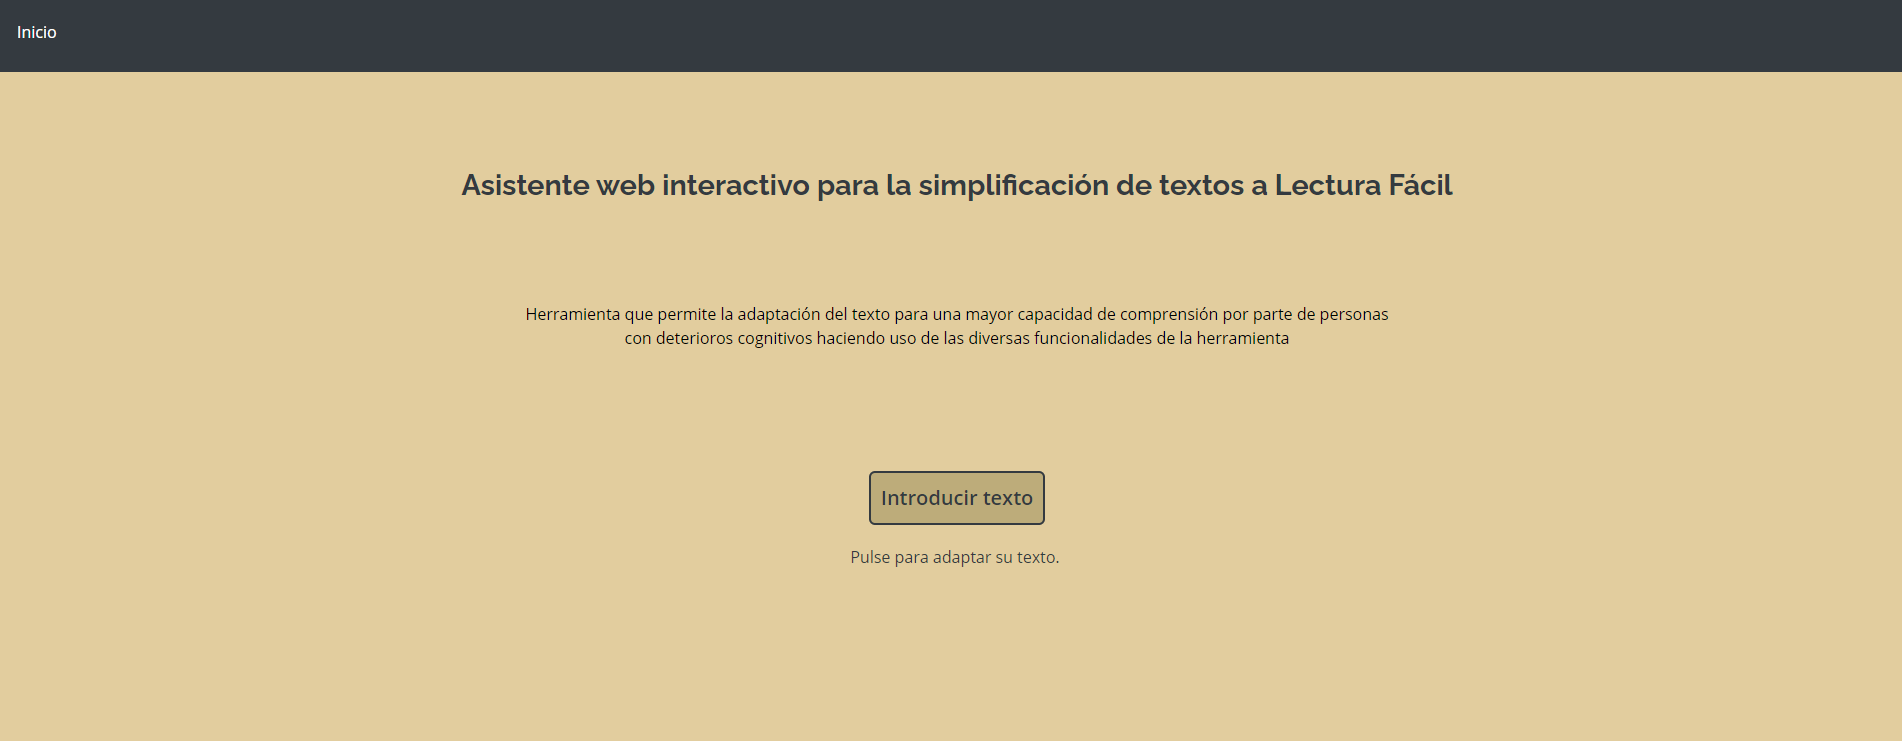
\includegraphics[scale=1]{Imagenes/Figuras/InterfazInicial}
 	
 	
 	\caption{Interfaz inicial del asistente.}
 	\label{fig:interfazInicial}
 \end{figure}
 
 Al pulsar en dicho botón se mostrará un panel lateral con las siguientes opciones:
 
 \begin{itemize}
 	\item \textbf{Texto original}: un  panel donde se introducirá el texto que queremos adaptar (ver Figura \ref{fig:interfazIntroduccionTexto}).
 	\begin{figure}[h!]
 		\centering
 		
 		
 		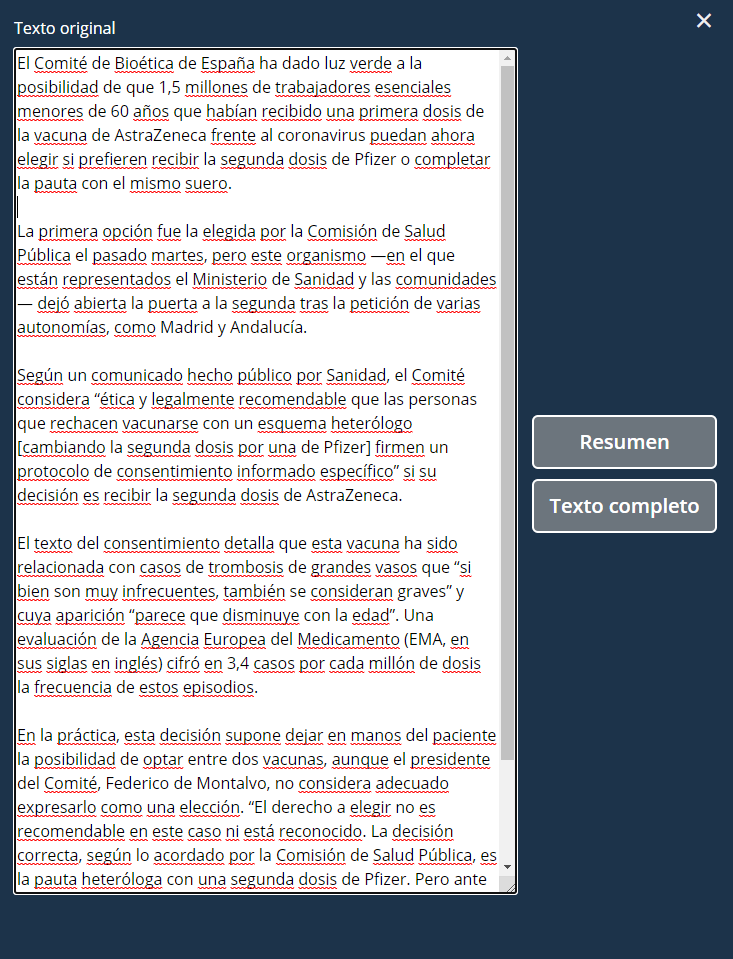
\includegraphics[scale=0.7]{Imagenes/Figuras/PanelIzquierdo}
 		
 		
 		\caption{Introducción de texto.}
 		\label{fig:interfazIntroduccionTexto}
 	\end{figure}
 	 	\item \textbf{Botón (Resumen)}: si pulsamos esta opción se mostrará una vista con una serie de frases seleccionables partiendo del resumen del texto original previamente introducido (véase Figura \ref{fig:interfazFraseTextoResumido}). Este botón permanecerá inactivo hasta que se introduzca texto. 
 	 	 	\item \textbf{Botón (Texto completo)}: si, por el contrario, pulsamos esta opción se mostrará el texto completo dividido en frases, también seleccionables (Figura \ref{fig:interfazIntroducirCompleto}). Al igual que el anterior botón también permanecerá inactivo hasta que el usuario introduzca texto. 
 	 	 \begin{figure}[h!]
 	 	 	\centering
 	 	 	
 	 	 	
 	 	 	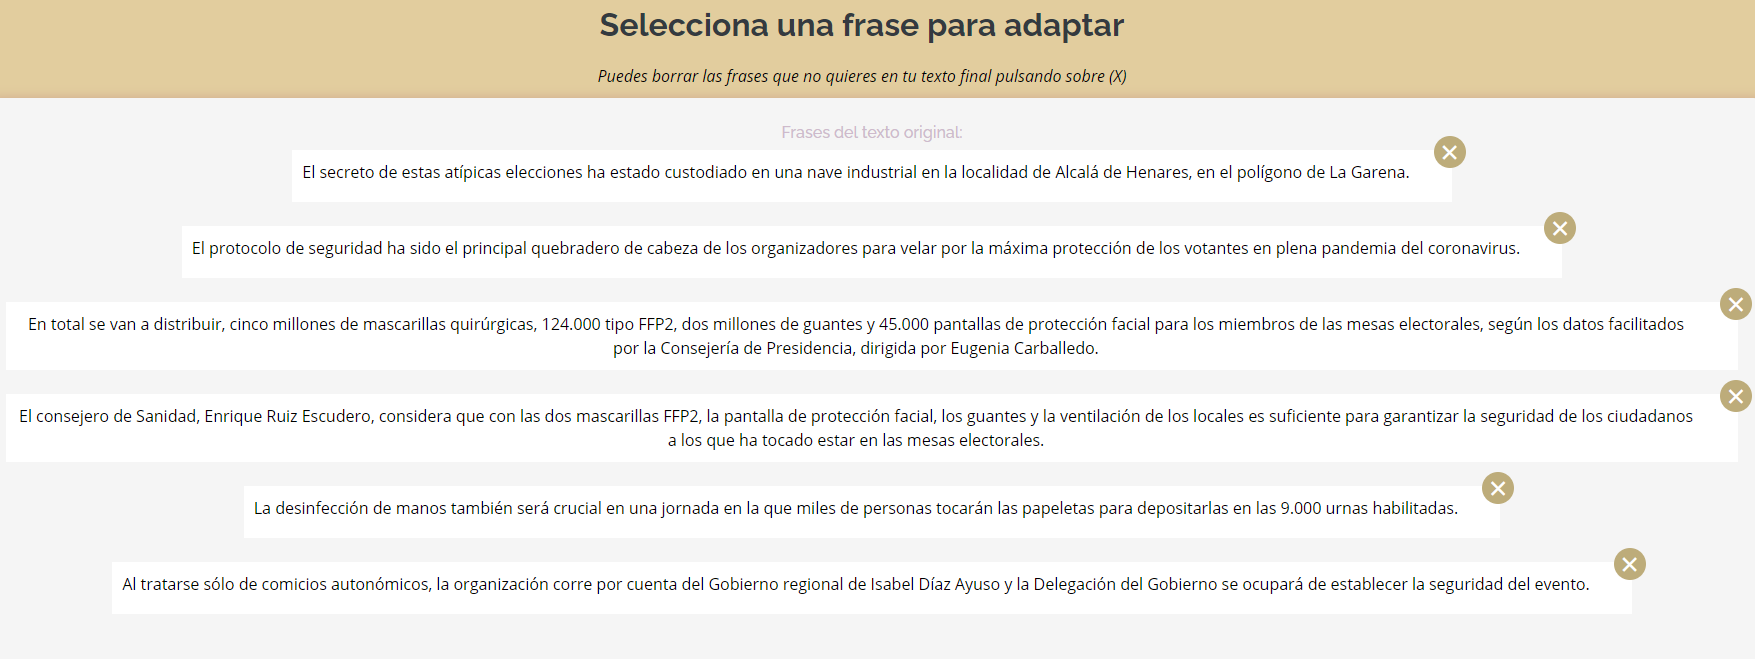
\includegraphics[scale=0.7]{Imagenes/Figuras/Resumen}
 	 	 	
 	 	 	
 	 	 	\caption{Frases partiendo del resumen.}
 	 	 	\label{fig:interfazFraseTextoResumido}
 	 	 \end{figure}
 	 	 
 	 	 
 	 	 \begin{figure}[h!]
 	 	 	\centering
 	 	 	
 	 	 	
 	 	 	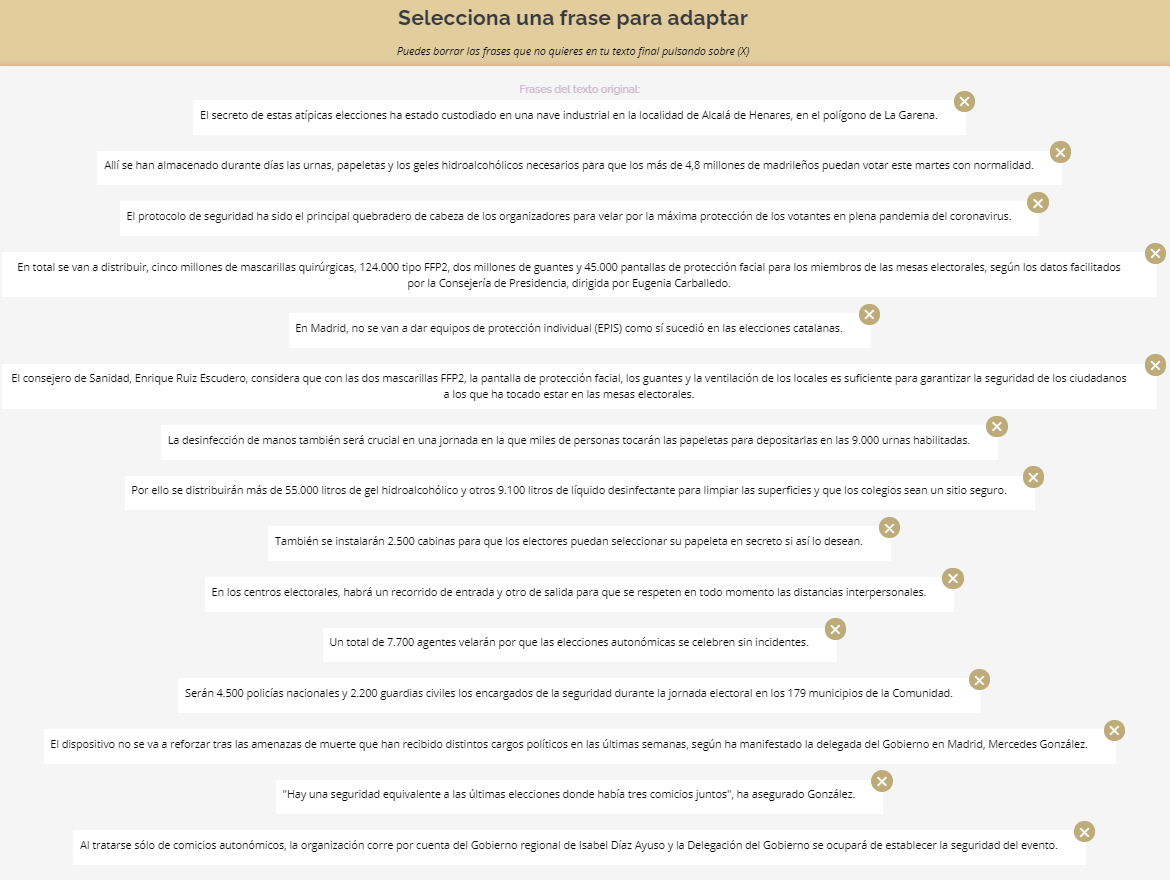
\includegraphics[scale=0.7]{Imagenes/Figuras/TextoCompleto}
 	 	 	
 	 	 	
 	 	 	\caption{Frases partiendo del texto completo.}
 	 	 	\label{fig:interfazIntroducirCompleto}
 	 	 \end{figure}	
 \end{itemize}

	Recordemos que en la Figura \ref{fig:interfazInicial} sólo contábamos con la pestaña de ``Inicio'' en la barra de navegación, la cuál cambia añadiendo una nueva pestaña \textbf{``Texto original''}. Esta pestaña nos permitirá consultar siempre el texto original que hemos introducido y cambiar en cualquier punto del flujo la opción elegida detallada anteriormente (resumen o texto completo). 


\section{Adaptaciones sobre frases}

Al clicar  sobre una frase se cambiará a una vista donde aparecerá el árbol de dependencias (véase Figura \ref{fig:arbolDependencias}), que describe la estructura sintáctica de dicha frase, que le servirá al editor a la hora de adaptarla de una manera interactiva. 

En dicho árbol encontramos las unidades léxicas separadas de la frase, las cuales podremos pulsar y realizar una serie de operaciones (botones) que se encuentran en la parte inferior izquierda. Junto a estos, aparece una breve explicación de la funcionalidad (ver operaciones que podemos efectuar en la Figura \ref{fig:botonesFuncionales}) que detallaremos en el capitulo XX. 

En la parte superior de la pantalla el editor podrá visualizar en todo momento la frase previamente elegida y un enlace (\textbf{Volver a las frases}) para volver al listado de frases, en el caso de que se quiera elegir otra o retomar alguna que ya haya sido modificada.

 En la parte inferior derecha de la vista, tenemos el borrador del texto final (Ver Figura \ref{fig:borradorTextoFinal}) donde se puede visualizar la transformación de la frase seleccionada (en negrita) habiendo realizado, o no, las diferentes operaciones. 
\begin{figure}[h!]
	\centering	
	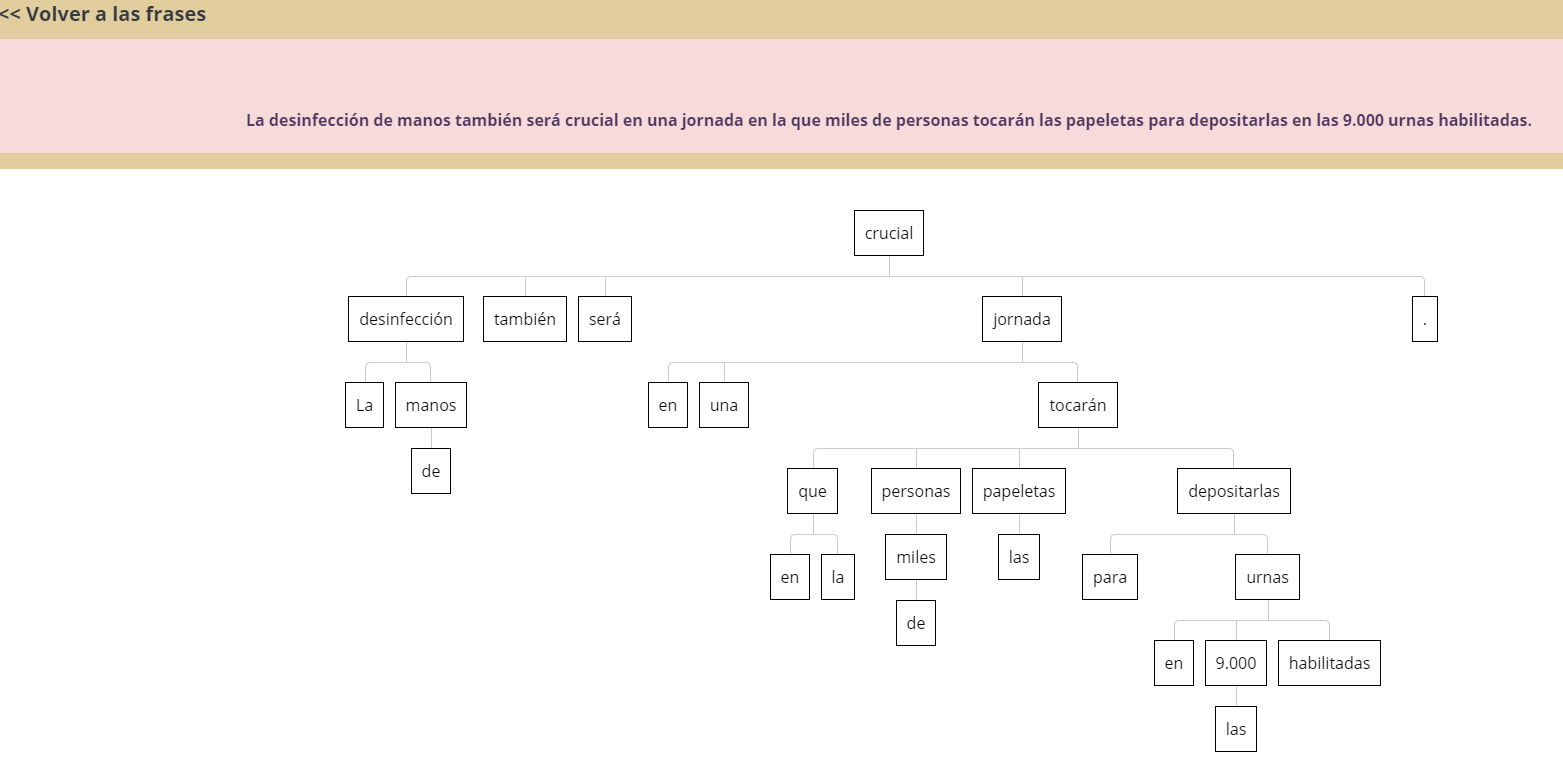
\includegraphics[scale=0.7]{Imagenes/Figuras/arbol}	
	\caption{Árbol de dependencias.}
	\label{fig:arbolDependencias}
\end{figure}
\begin{figure}[h!]
	\centering
	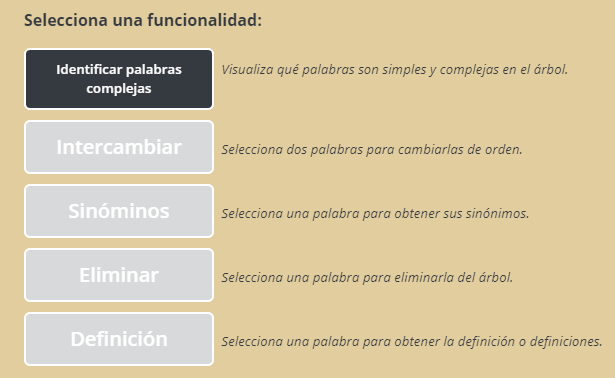
\includegraphics[scale=1.0]{Imagenes/Figuras/botonesFuncionales}
	\caption{Operaciones que podemos efectuar en el árbol de dependencias}
	\label{fig:botonesFuncionales}
\end{figure}
\begin{figure}[h!]
	\centering
	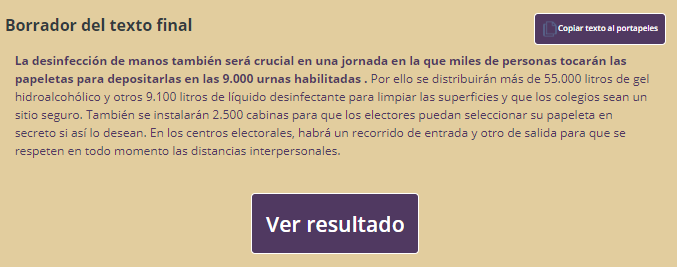
\includegraphics[scale=1.0]{Imagenes/Figuras/borradorTextoFinal}
	\caption{Borrador del texto final.}
	\label{fig:borradorTextoFinal}
\end{figure}


A continuación, describiremos en qué consisten, en qué situaciones y cómo el usuario debe utilizar cada una de las operaciones que se pueden efectuar.

\subsection{Palabras complejas}
Esta funcionalidad es de utilidad cuando el editor desee conocer aquellos términos de la frase que pueden ser susceptibles de ser reemplazados por sinónimos que sean más asequibles de comprender para el lector. El elemento visual que se encargará de esta función es el botón \textbf{Identificar palabras complejas}.

Una vez hagamos clic en este botón nuestro árbol de dependencias mostrará las palabras complejas. Como podemos ver en la Figura \ref{fig:palabrasComplejas}, aparece una leyenda en la parte superior izquierda del árbol, indicando el color en el que se colorean las complejas. Una vez pulsado, el texto del botón cambiará a \textbf{Desactivar palabras complejas} para poder volver a la vista original del árbol de dependencias.  
	 \begin{figure}[h!]
	\centering
	
	
	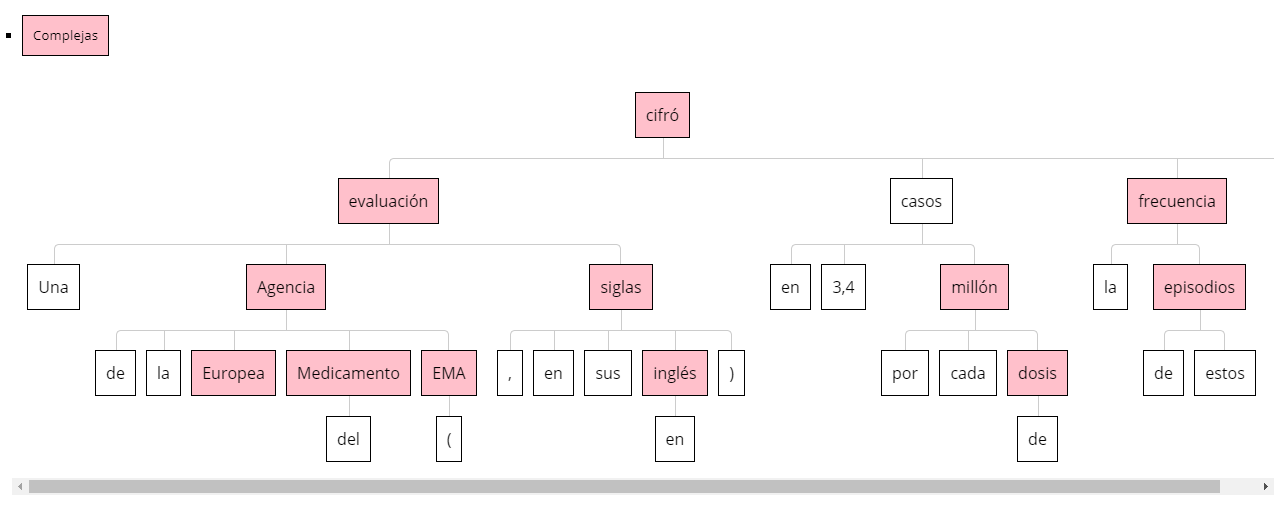
\includegraphics[scale=0.7]{Imagenes/Figuras/palabrasComplejas}
	
	
	\caption{Palabras complejas resaltadas en el árbol.}
	\label{fig:palabrasComplejas}
\end{figure}
\subsection{Intercambio de partes en el árbol de dependencias}
En caso de que el editor desee modificar el orden sintáctico de la frase, por ejemplo, se puede dar la situación de que la segunda parte de una frase sea más importante y por ende se quiera que el lector ponga más atención a esa parte. 

Para que esta funcionalidad se active es necesaria tener seleccionadas dos palabras del árbol. Ambas palabras cambiarán de orden incluyendo también aquellas que dependan de la misma (intercambio de dos palabras en el árbol de dependencias en las Figuras \ref{fig:eleccionIntercambio} y \ref{fig:intercambio}). El texto resultante quedaría como se muestra en la Figura \ref{fig:borradorIntercambio}
\begin{figure}[h!]
	\centering
	
	
	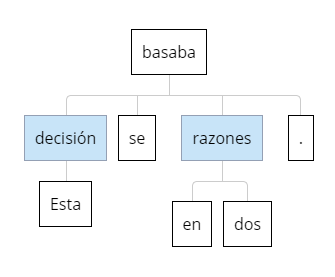
\includegraphics[scale=1]{Imagenes/Figuras/EleccionIntercambio}
	
	
	\caption{Elección de dos palabras para el intercambio.}
	\label{fig:eleccionIntercambio}
\end{figure}
\begin{figure}[h!]
	\centering
	
	
	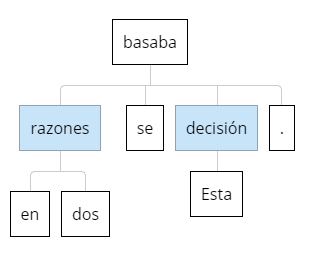
\includegraphics[scale=1]{Imagenes/Figuras/IntercambioArbol}
	
	
	\caption{Árbol de dependencias después del intercambio.}
	\label{fig:intercambio}
\end{figure}
\begin{figure}[h!]
	\centering
	
	
	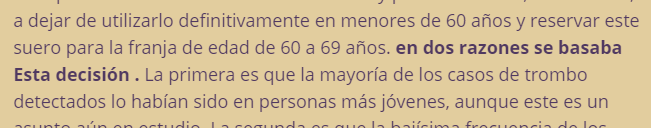
\includegraphics[scale=1]{Imagenes/Figuras/BorradorIntercambio}
	
	
	\caption{Resultado en el borrador del texto final tras el intercambio.}
	\label{fig:borradorIntercambio}
\end{figure}
\subsection{Sinónimos}
En ocasiones el usuario se verá en la necesidad de realizar una simplificación léxica sustituyendo una palabra por un sinónimo más conocido. Podrá hacer uso de ella, pulsando sobre el botón (\textbf{Sinónimos}), siempre y cuando se haya seleccionado una palabra del árbol previamente. Una vez pulsado, se muestra, si los tiene, todos los sinónimos de la palabra elegida. En caso de que la palabra no tenga sinónimos aparecerá un texto informando que carece de ellos. Si los tiene, se mostrará un listado de estos indicando cuáles son sencillos y cuáles no (ver opción sinónimos en la Figura \ref{fig:listaSinonimos}).

	 \begin{figure}[h!]
	\centering
	
	
	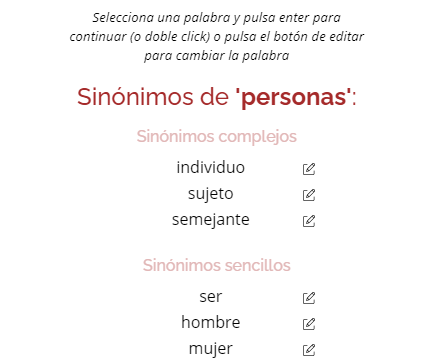
\includegraphics[scale=1.0]{Imagenes/Figuras/SinonimoPersona}
	
	
	\caption{Lista de sinónimos de una palabra seleccionada}
	\label{fig:listaSinonimos}
\end{figure}

 Llegados a este punto, se podrá seleccionar uno de ellos o bien haciendo doble clic o bien editándolo si fuese necesario para un significado coherente con la frase (concordancia en género, número, persona y conjugación), y posteriormente pulsar ``Enter'' para el cambio (véase la Figura \ref{fig:edicionSinonimos}).


\begin{figure}[h!]
\centering


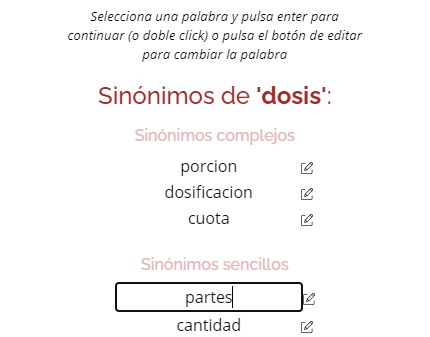
\includegraphics[scale=1.0]{Imagenes/Figuras/EditarSinonimo}


\caption{Interfaz de edición de sinónimos}
\label{fig:edicionSinonimos}
\end{figure}
Al hacer doble clic o ``Enter'', si lo hemos editado, se mostrará una ventana de diálogo (Aceptar y Cancelar) para asegurar si es realmente la acción que queremos realizar (ver Figura \ref{fig:modalSinonimos}). En el caso de que se elija ``Aceptar'', tanto en el árbol de dependencias como en el borrador del texto final se reemplazará la palabra (Figura \ref{fig:resultadoSinonimos}). En caso contrario, no habrá modificación alguna.

\begin{figure}[h!]
	\centering
	
	
	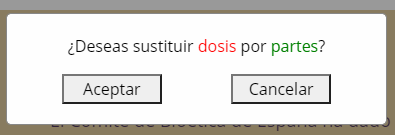
\includegraphics[scale=1.0]{Imagenes/Figuras/modalSinonimos}
	
	
	\caption{Ventana de diálogo de reemplazo de sinónimo.}
	\label{fig:modalSinonimos}
\end{figure}

\begin{figure}[h!]
	\centering
	
	
	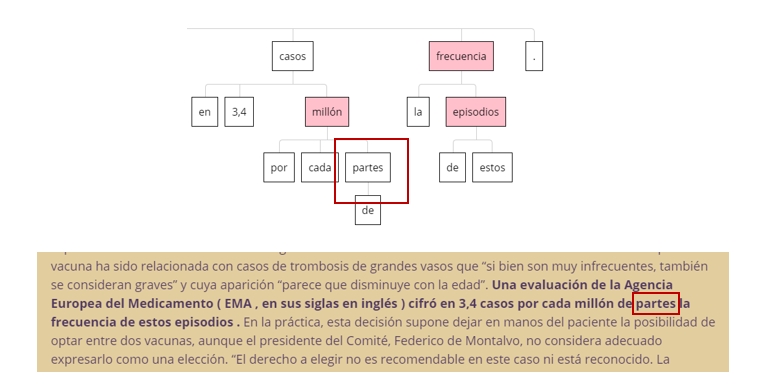
\includegraphics[scale=1.3]{Imagenes/Figuras/CambioSinonimoArbolBorrador}
	
	
	\caption{Resultado de reemplazo del sinónimo tanto en el árbol de dependencias como en el borrador}
	\label{fig:resultadoSinonimos}
\end{figure}
\subsection{Eliminar partes en el árbol de dependencias}

El editor puede encontrarse con frases que no requieren de ciertas palabras para que se capte la esencia de las mismas por parte del lector. Es por ello, por lo que tiene la opción de eliminar términos a su disposición. Es necesario seleccionar una palabra del árbol para que esta funcionalidad pueda llevarse a cabo. Suprime tanto a ella como aquellas que dependan de la misma. En las Figuras \ref{fig:eliminacionPrevia} y \ref{fig:eliminacion}, vemos la palabra seleccionada que queremos eliminar y el resultado de su eliminación en el árbol y en el texto del borrador final.
	 \begin{figure}[h!]
	\centering
	
	
	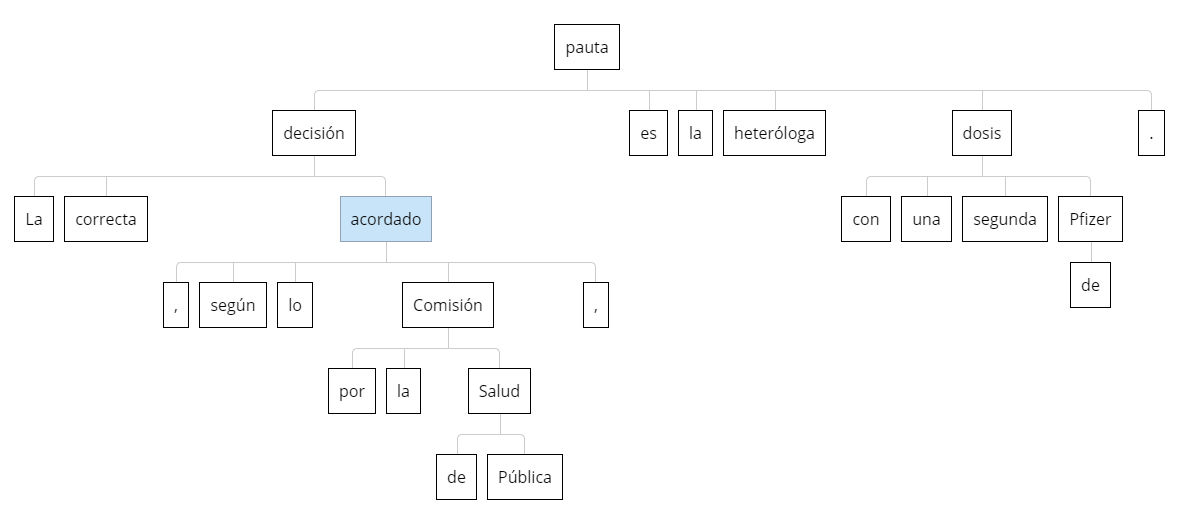
\includegraphics[scale=0.8]{Imagenes/Figuras/EleccionEliminacion}
	
	
	\caption{Árbol antes la eliminación de una palabra.}
	\label{fig:eliminacionPrevia}
\end{figure} 
	 \begin{figure}[h!]
	\centering
	
	
	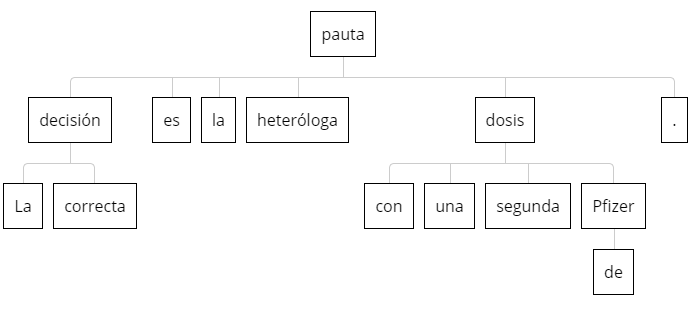
\includegraphics[scale=0.9]{Imagenes/Figuras/EliminacionSubarbol}
	
	
	\caption{Árbol tras la eliminación de una palabra.}
	\label{fig:eliminacion}
\end{figure} 
El resultado de cómo quedaría la frase lo podemos ver en la Figura \ref{fig:resultadoEliminar}.
	 \begin{figure}[h!]
	\centering
	
	
	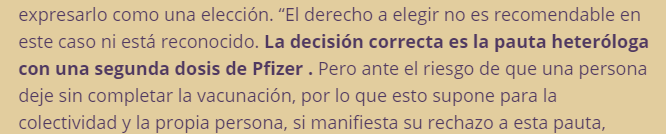
\includegraphics[scale=1]{Imagenes/Figuras/BorradorEliminacion}
	
	
	\caption{Borrador del texto final tras la eliminación de una palabra.}
	\label{fig:resultadoEliminar}
\end{figure} 

\subsection{Definiciones respecto a una palabra}
 Gracias a esta funcionalidad, el usuario podrá nutrir el texto final con definiciones de uno o varios términos. 
 
 Seleccionando una palabra en el árbol, el botón (\textbf{Definición}) se activará. Al pulsar sobre este se mostrará un listado con todas las acepciones, si las tiene, de la palabra seleccionada (Figura \ref{fig:definiciones}). Haciendo clic en una de ellas, ésta se adjuntará a modo glosario como parte del texto final, sirviendo de apoyo a la comprensión del mismo (ver Figura \ref{fig:definicionesBorrador}). En caso de que no posea definiciones (por ejemplo, nombres propios) aparecerá un texto informando que carece de ellas.
 	 \begin{figure}[h!]
 	\centering
 	
 	
 	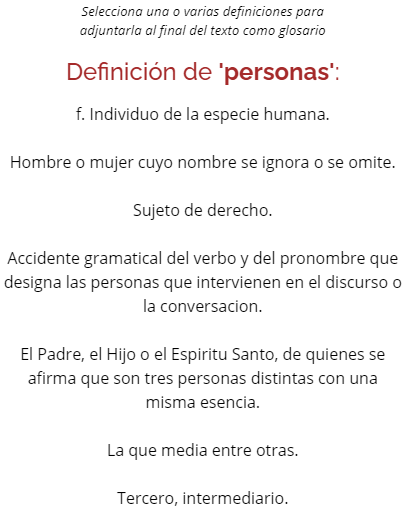
\includegraphics[scale=0.8]{Imagenes/Figuras/DefinicionesPersonas}
 	
 	
 	\caption{Listado de las definiciones}
 	\label{fig:definiciones}
 \end{figure}
 	 \begin{figure}[h!]
	\centering
	
	
	\includegraphics[scale=0.8]{Imagenes/Figuras/GlosarioBorrador}
	
	
	\caption{Glosario adjunto al borrador del texto final.}
	\label{fig:definicionesBorrador}
\end{figure}
\subsection{Resultado de la adaptación}
 
Cuando hayamos considerado que el texto esté adaptado a nuestras necesidades, podemos visualizarlo haciendo clic en el botón (\textbf{Ver resultado}), el cuál lo encontramos en la parte inferior derecha del borrador del texto final (ver Figura \ref{fig:botonResultado}). Al pulsarlo, desplegará un panel, el cual es editable, en la parte derecha con el mismo texto que obtuvimos en el borrador (este panel lo podemos ver en la Figura \ref{fig:panelFinal}). Esto es útil, por ejemplo, si el editor desea incluir el glosario dentro del contexto de las frases (Figura \ref{fig:}). 
\begin{figure}[h!]
	\centering
	
	
	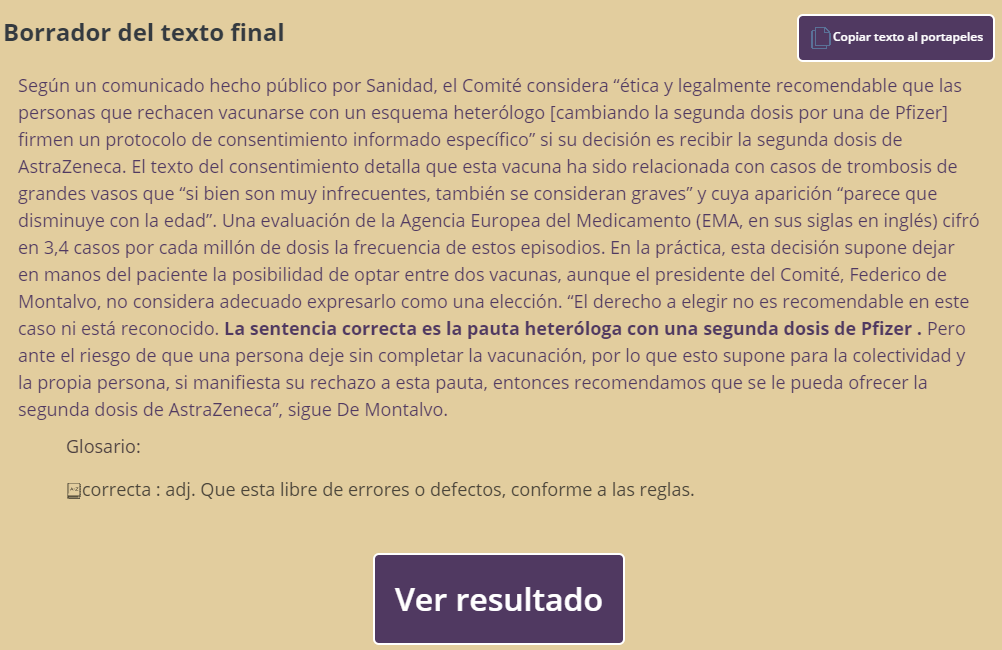
\includegraphics[scale=0.8]{Imagenes/Figuras/verResultado}
	
	
	\caption{Botón Ver resultado junto al borrador del texto final.}
	\label{fig:botonResultado}
\end{figure}
\begin{figure}[h!]
	\centering
	
	
	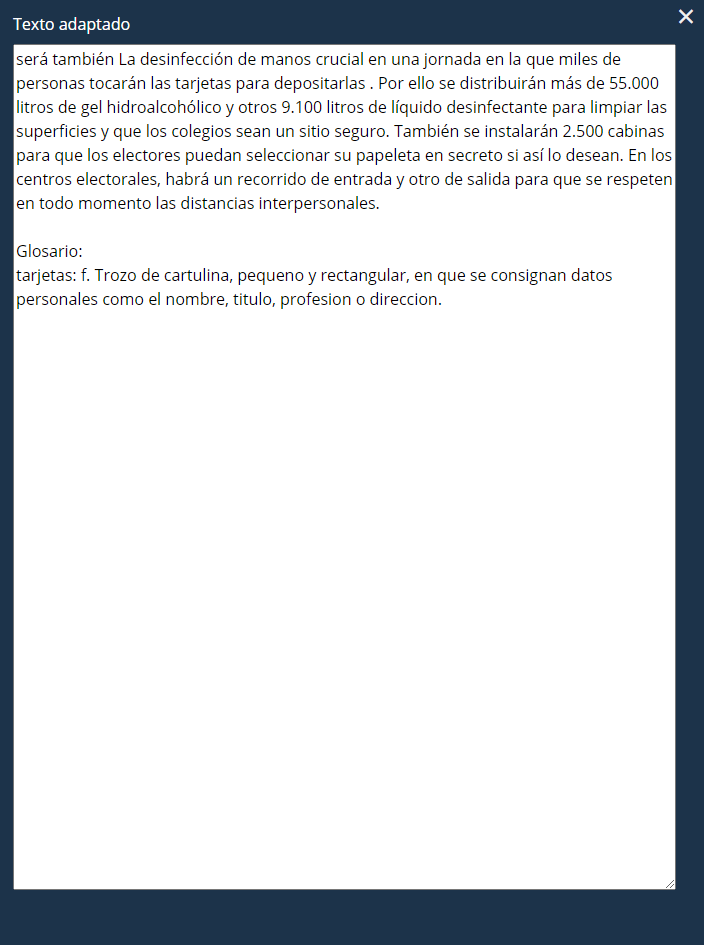
\includegraphics[scale=0.8]{Imagenes/Figuras/PanelDerecho}
	
	
	\caption{Panel con el resultado final del texto adaptado}
	\label{fig:panelFinal}
\end{figure}

Como hemos visto en la Figura \ref{fig:botonResultado}, también contamos con un botón (\textbf{Copiar al portapapeles}) que nos da la opción de copiar el texto del borrador para poder introducirlo en cualquier herramienta externa.



	\chapter{Implementación}
\label{cap:implementacion}

\chapterquote{Puede que tengas grandes ideas en la cabeza, pero lo que importa es la acción. Una idea, si no se lleva a cabo, no producirá ninguna manifestación, ni resultados ni recompensas}{Miguel Ruiz}


En este capítulo hacemos una descripción detallada sobre la arquitectura en la que está basada nuestro asistente. Hablaremos también sobre la implementación de las distintas funcionalidades (ver sección XXXX) que se ha llevado a cabo tanto en la parte Back End como Front End.


\section{Arquitectura}

La estructura de nuestro proyecto está soportado sobre un entorno Flask, teniendo el nivel de directorios que se muestra en la Figura \ref{fig:projectStructure}.

	 \begin{figure}[h!]
	\centering
	
	
	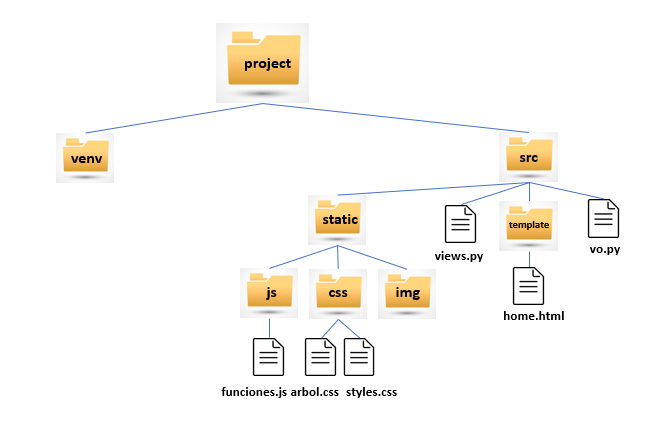
\includegraphics[scale=1.2]{Imagenes/Figuras/Project-Structure}
	
	
	\caption{Estructura del proyecto en Flask}
	\label{fig:projectStructure}
\end{figure}

A continuación, se explican la función de cada uno de los ficheros que componen la aplicación web.

\subsection{Ficheros del entorno}

Los ficheros principales son:
\begin{itemize}
	\item \textbf{views.py}: es el encargado de la lógica de todos los endpoints de la aplicación, así como el renderizado de la plantilla. Cada uno de esos endpoints tendrá una funcionalidad distinta, los cuales serán llamados por una función de funciones.js 
	\item \textbf{vo.py}: se encarga de la organización de clases.
	\item \textbf{home.html}: en este archivo creamos la estructura de nuestro asistente y la organización que mostrará el contenido.
	\item \textbf{funciones.js}: la misión de este fichero es comunicar la aplicación web con los elementos del DOM de la misma, haciendo posible la modificación del HTML dinámicamente. Las modificaciones que efectuamos en este archivo es añadir nuevas etiquetas, modificando o eliminando otras, cambiar sus atributos, añadiendo clases, cambiar el contenido de texto, etc. También es el encargado de la comunicación con la vista (views.py) para la petición y respuesta de servicios web.
	\item \textbf{arbol.css}: archivo encargado de generar los estilos para que nuestro árbol de dependencias tenga la apariencia de un árbol genealógico.
	\item \textbf{style.css}: fichero encargado de dar estilos a todo lo que concierne nuestra aplicación web excepto el árbol de dependencias (fuentes, disposición, tamaños, colores, etc.)   
\end{itemize}

\subsection{Servicios web externos}\label{sec:serviciosWebExternos}
Para hacer uso de las principales funcionalidades descritas en la sección XXX, contamos con una arquitectura de servicios web REST basada en endpoints (URLs), intercambiando mensajes entre cliente y servidor (Figura \ref{fig:apiRest}). 

\begin{figure}[h!]
	\centering
	
	
	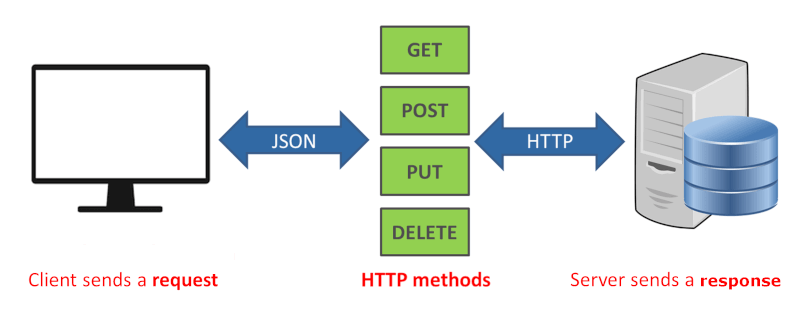
\includegraphics[scale=0.4]{Imagenes/Figuras/rest_api}
	
	
	\caption{Servicio REST cliente/servidor}
	\label{fig:apiRest}
\end{figure}

Un servicio web REST es una interfaz para conectar varios servicios web basados en el protocolo HTTP que define una gran cantidad de métodos, de los cuales describimos los cuatro más básicos:
\begin{itemize}
	\item \textbf{GET}: se utiliza para acceder a los distintos recursos. Si requiere del envío de un parámetro al servidor (URI param), éste se pasa como un elemento en la URI (del inglés, \textit{Uniform Resource Identifier}). 
	
	\item \textbf{POST}: se usa para realizar acciones de creación de nuevos recursos. Si se requiere el envío de información al servidor, esta se pasa dentro del cuerpo de la petición HTTP (body param).
	
	\item \textbf{PUT}: se utiliza para la modificación de los recursos existentes. Puede enviar parámetros tanto en la URI como en el cuerpo de la petición HTTP.
	
	\item \textbf{DELETE}: se utiliza para la eliminar los recursos existentes, siendo la operación análoga al POST. El parámetro será informado a través de la URI.
\end{itemize}

Estas métodos pueden ser usados en distintas situaciones devolviendo los datos en distintos formatos como XML y JSON.
En nuestro caso, hemos usado el formato JSON.

Nuestra arquitectura REST tiene el aspecto como muestra la Figura \ref{fig:ArquitecturaAsistenteR}, que a continuación describimos.
\begin{figure}[h!]
	\centering
	
	
	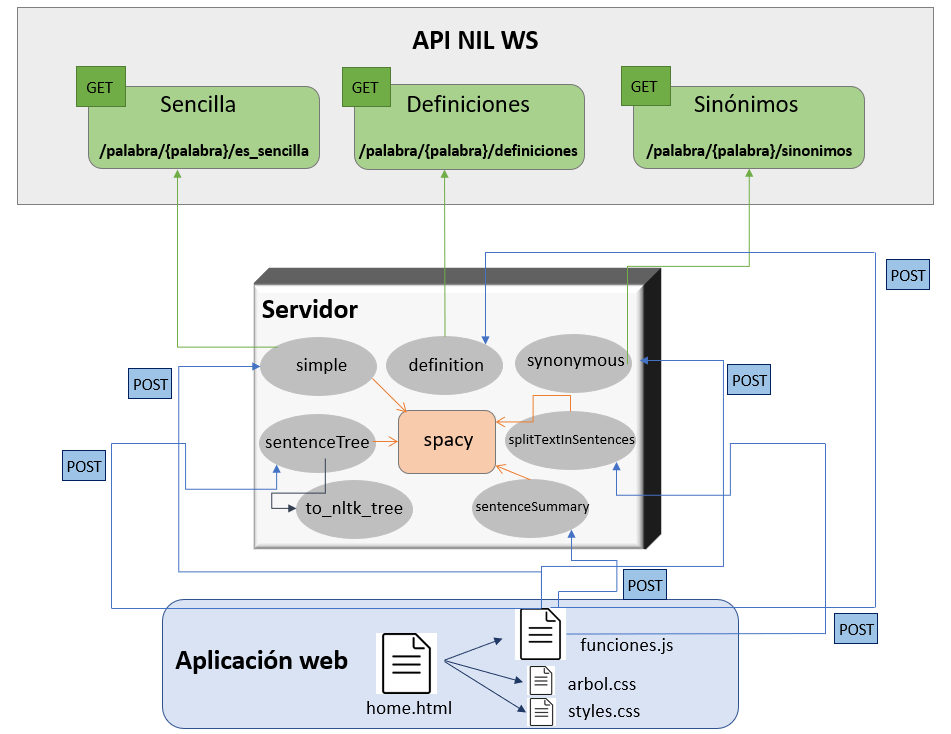
\includegraphics[scale=0.9]{Imagenes/Figuras/ArquitecturaAsistenteR}
	
	
	\caption{Diagrama de la arquitectura REST del asistente web}
	\label{fig:ArquitecturaAsistenteR}
\end{figure}

  Hacemos uso de los siguientes servicios REST que nos ofrece la API del grupo NIL\footnote{Para más información acceder a \href{https://holstein.fdi.ucm.es/nil-ws-api/}{https://holstein.fdi.ucm.es/nil-ws-api/}} (descrita en el capítulo X sección XXX):


	


\begin{itemize}
	\item \textbf{Servicio para comprobar si una palabra es compleja}.
	\begin{lstlisting}[backgroundcolor = \color{pink},
	xleftmargin = 1cm,
	framexleftmargin = 1em,frame=tlbr,framesep=4pt,framerule=1pt]
	GET https://holstein.fdi.ucm.es/nil-ws-api/palabra/
	{palabra}/es\_sencilla
	
	
\end{lstlisting}
	
	Este recurso devuelve un objeto en formato JSON que contiene el campo ``palabraSencilla'' de tipo booleano que en el caso que sea False la palabra introducida a través de la URI es compleja (ver Figura \ref{fig:apiSencilla}).
		 \begin{figure}[h!]
		\centering
		
		
		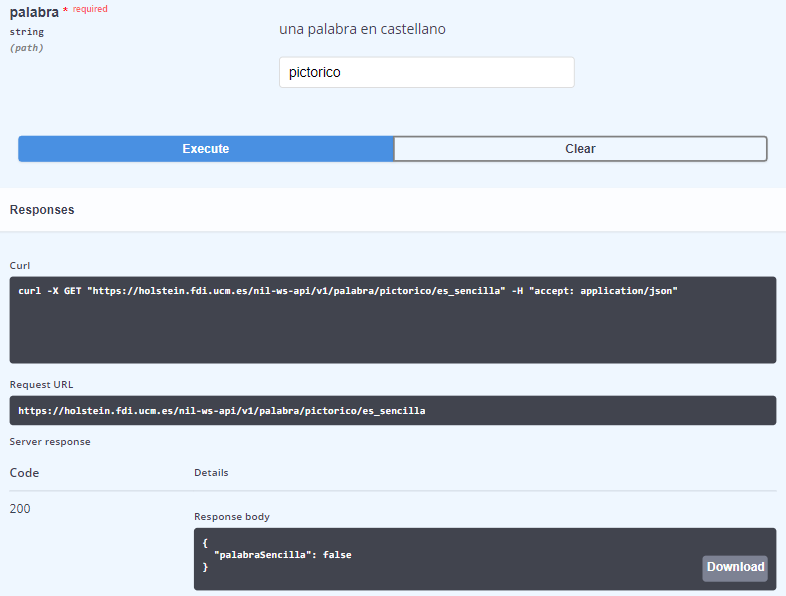
\includegraphics[scale=1]{Imagenes/Figuras/APISencilla}
		
		
		\caption{Petición para comprobar si una palabra es compleja}
		\label{fig:apiSencilla}
	\end{figure}
	\item \textbf{Servicio para obtener definiciones de una palabra}.
\newline

	\begin{lstlisting}[backgroundcolor = \color{pink},
	xleftmargin = 1cm,
	framexleftmargin = 1em,frame=tlbr,framesep=4pt,framerule=1pt]
	GET https://holstein.fdi.ucm.es/nil-ws-api/palabra/
	{palabra}/definiciones

	
	
\end{lstlisting}




En este caso, el servicio devuelve un objeto JSON que contiene el campo ``definiciones'' de tipo arrayList en el que en cada posición hay otro objeto, ``definicion'', cuyo valor es de tipo string con la acepción correspondiente (ver Figura \ref{fig:apiDefinicion}).
\begin{figure}[h!]
	\centering
	
	
	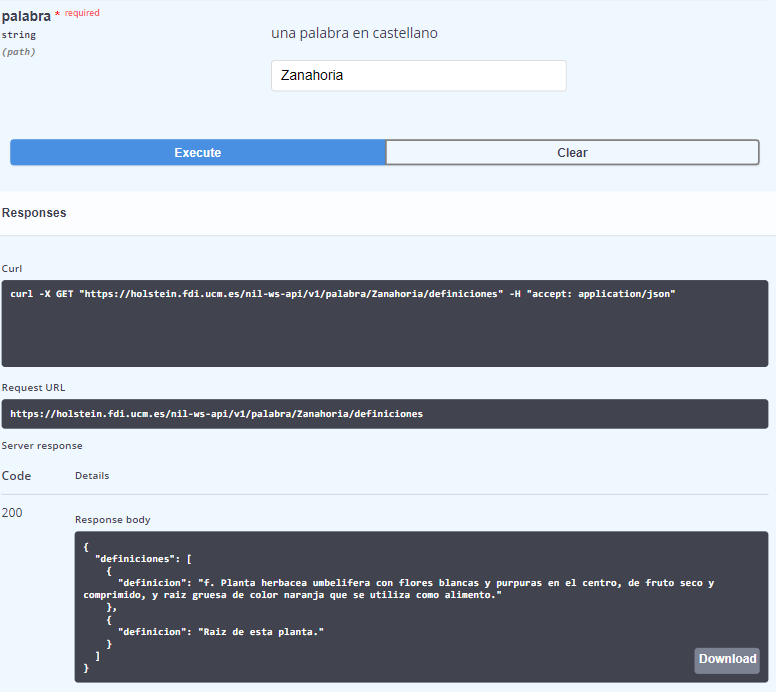
\includegraphics[scale=1]{Imagenes/Figuras/ApiDefinicion}
	
	
	\caption{Petición que devuelve una lista de definiciones}
	\label{fig:apiDefinicion}
\end{figure}
	\item \textbf{Servicio para obtener sinónimos de una palabra}.
	\begin{lstlisting}[backgroundcolor = \color{pink},
	xleftmargin = 1cm,
	framexleftmargin = 1em,frame=tlbr,framesep=4pt,framerule=1pt]
	GET https://holstein.fdi.ucm.es/nil-ws-api/palabra/
	{palabra}/sinonimos	
	
	
	
	
\end{lstlisting}



El servicio devuelve un objeto JSON que contiene el campo ``sinonimos'' de tipo arrayList en el que en cada posición hay otro objeto, ``sinonimo'', cuyo valor es de tipo string con la acepción correspondiente (ver Figura \ref{fig:apiSinonimo}).
\begin{figure}[h!]
	\centering
	
	
	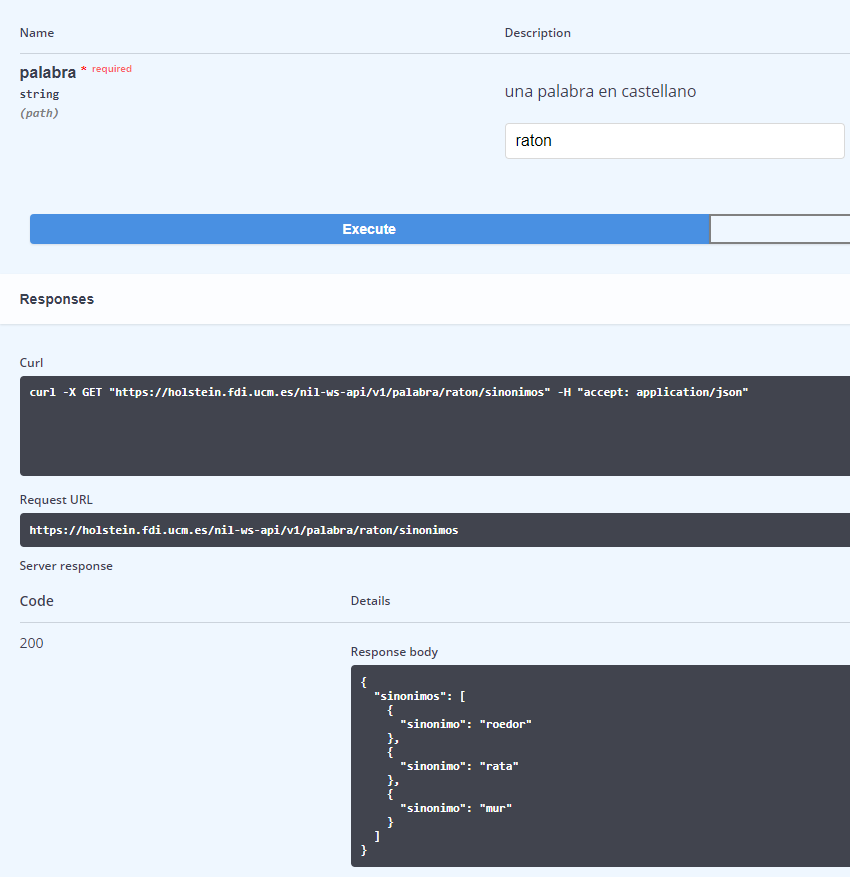
\includegraphics[scale=1]{Imagenes/Figuras/APISinonimos}
	
	
	\caption{Petición que devuelve una lista de sinónimos}
	\label{fig:apiSinonimo}
\end{figure}
\end{itemize}

Cabe destacar que esta API no hace uso de las reglas de acentuación, de manera que debemos de insertar las palabras sin tildes (obsérvese la Figura \ref{fig:apiSinonimo}).

\subsection{Librería Spacy}

\subsection{Implementaciones del servidor}

\subsection{Implementaciones de la aplicación web}

En esta sección se explica en detalle como han sido desarrolladas las funcionalidades (capítulo \ref{cap:asistenteWeb} \ref{sec:}) de la aplicación web, cuya finalidad es proporcionar al usuario una interfaz sencilla, donde puedan introducir un texto, hacer una serie de transformaciones para obtener el mismo simplificado a Lectura Fácil.


Para que el contenido de la aplicación web sea dinámico se ha desarrolla con JavaScript, cambiando según la acción del usuario. Estás acciones son:

\begin{itemize}
	\item Botón (\textbf{Resumen}): se realiza una llamada Fetch al endpoint ``/summary'' con el texto completo previamente introducido. La respuesta recibida será un objeto JSON, el cuál contiene el resumen del texto. Posteriormente se hará otra llamada Fetch al endpoint ``/sentences'', que devuelve el texto en frases. Estás frases se incrustan en el código HTML, escribiéndolas a modo de lista (una debajo de otra).    
 
	\item Botón (\textbf{Texto completo}): a diferencia de botón anterior este hace una llamada únicamente al endpoint ``/sentences'', devolviendo el texto completo en frases.

	\item Creación del árbol de dependencias: se realiza una llamada Fetch al endpoint ``/sentences/tree'', devolviendo así un objeto JSON con la estructura del árbol. Para su construcción de este, hemos usado un algoritmo de búsqueda en profundidad (BFS), recorriendo todos los nodos (en nuestro caso palabras de la frase). El funcionamiento de este algoritmo consiste en ir expandiendo cada uno de sus nodos desde la raíz hacia el nodo hoja (no tiene más hijos) de manera recurrente (Figura \ref{fig:diagramaBFS}).
	\begin{figure}[h!]
		\centering
		
		
		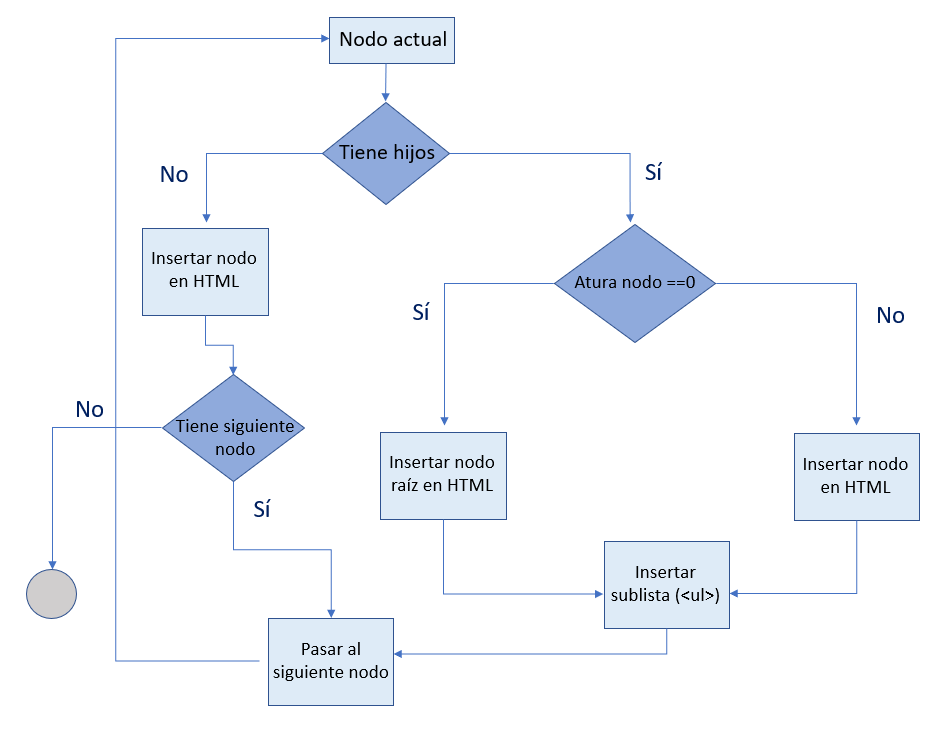
\includegraphics[scale=1]{Imagenes/Figuras/diagramaBFS}
		
		
		\caption{Petición que devuelve una lista de sinónimos}
		\label{fig:diagramaBFS}
	\end{figure}
	
		Por ejemplo, supongamos que queramos adaptar la frase ``También se instalarán 2.500 cabinas para que los electores puedan seleccionar su papeleta en secreto si así lo desean.'', el objeto JSON tendría el aspecto de la Figura \ref{fig:objetoJSON}. 
	Cada nodo contiene los siguientes datos:
		\begin{itemize}
		\item \textbf{children}: array de nodos hijos.
		\item \textbf{height}: nivel del nodo con respecto a la raíz (en nuestro ejemplo ``instalarán'' sería nuestra raíz, que tiene una altura 0).
		\item \textbf{id}: identificador único de cada nodo.
		\item \textbf{text}: palabra propia del nodo.
	\end{itemize}
En la Figura \ref{fig:arbolDependencias} observamos el árbol con el que podremos interactuar durante la adaptación.
	\item Palabras complejas.
	\item 
\end{itemiz
	%\include{Capitulos/Capitulo5}
	\chapter{Conclusiones y Trabajo Futuro}
\label{cap:conclusiones}

Conclusiones del trabajo y líneas de trabajo futuro.



	\chapter{Trabajo individual}
\label{cap:trabajoIndividual}

\section{Estefanía Ortega Ávila}

En primer lugar, mi labor en este TFG se centró en una investigación de las tareas y los pasos a seguir que se llevan a cabo para adaptar un texto a Lectura Fácil. Para ello, consulté diversas webs y vídeos que me proporcionaran dicha información. De esta manera, entendí a qué público iba dirigida este tipo de lectura y qué técnicas eran las más utilizadas. 

Posteriormente, tanto mi compañero como yo, identificamos diferentes herramientas que podrían ser útiles para transformar textos, probando algunas de ellas, haciéndonos una idea de qué medios disponen los editores para realizar su labor.

Una vez realizada la investigación, mi compañero y yo comenzamos a estudiar las tecnologías que iban a hacer posible la implementación de nuestro asistente web. Optamos por hacer uso de servicios API REST, así como de la librería spaCy para el PLN.

Por otro lado, y esta es la que yo abordé, tenemos la implementación de la aplicación, es decir, la interfaz visual con el que el usuario editor interactuará y hará uso de las diferentes funcionalidades. 

Para el desarrollo de esta implementación, utilicé JavaScript para que los resultados de la llamada al servidor mediante una promesa Fetch a un endpoint me devolviera un objeto JSON que, al operar sobre él, plasme cierta información en la interfaz; usando HTML, para el desarrollo de la interfaz visual, y CSS para dar estilo a ésta (fuentes, tamaños, colores…).


La parte donde tuve más dificultad fue la de dibujar el árbol de dependencias con el aspecto de árbol genealógico y el poder procesar el objeto JSON que recibo del servidor para representar cada nodo con sus correspondientes dependencias. La solución por la que opté fue la de implementar un algoritmo BFS para poder recorrer el objeto, obteniendo la estructura de árbol deseada.

Otra parte de especial dificultad fue la relacionada con la funcionalidad ``Intercambiar'' en el caso de que se tuviera que modificar dos palabras independientes entre sí y, a su vez, las dependientes de éstas, reflejándose estos cambios en el borrador del texto final. Para solventarlo, hice uso de arrays auxiliares que me permitieron obtener el resultado que quería en el borrador para poder cambiar el texto dinámicamente.

Realicé algunas pruebas en Postman de los diferentes servicios de NIL-WS-API para validar que el comportamiento de la interfaz, se correspondía con lo que la API devolvía en su respuesta, por ejemplo, en el caso de comprobar que si una palabra se muestra de color rojo en el árbol, la API nos indique que dicha palabra es compleja. Esto me permitió, por primera vez, hacer uso de la herramienta Postman, la cual es bastante apropiada para el testeo de APIs.

Para el diseño de la interfaz del asistente, tomé en cuenta las recomendaciones de mis tutoras en las reuniones periódicas, sobre todo en lo que concierne a nombres de botones, elementos de la interfaz visibles o no visibles al pinchar en una determinada funcionalidad, etc.



Además de la implementación, me encargué de algunas de las partes que consta la memoria. En el capítulo 1, redacté los puntos relacionados con la motivación y los objetivos que persigue este asistente. El capítulo 2, los puntos 2.3 y 2.4 relacionados con proyectos, programas y aplicaciones en LF. Con respecto al capítulo 4, fui la persona encargada de desarrollarlo en su totalidad hablando sobre la aplicación y sus diferentes funcionalidades y vistas, mientras que del capítulo 5 fui la autora del punto 5.1 y 5.3, relacionados con la arquitectura y con la implementación del asistente, respectivamente. Finalmente, el capítulo 6, lo elaboré junto con la ayuda de mi compañero. Por último, traduje al inglés la parte de mi trabajo individual.



Por supuesto, se fue realizando modificaciones en aquellas partes que a nuestras tutoras les parecía que debíamos mejorar.

\section{Javier Sesé García}

Mi contribución al proyecto comenzó investigando a quién iba dirigida la Lectura Fácil y las formas que se utilizaban para adaptar textos. 

Posteriormente, nos centramos en el diseño de la arquitectura de la aplicación, la cual es una arquitectura REST basada en endpoints. Elegimos este diseño ya que nos pareció que es fácilmente ampliable en el caso de que se quisiera realizar un servicio nuevo.

Implementé esta arquitectura con Flask, del cual he adquirido los conocimientos para ser capaz de desplegar el servidor en él. He elegido Flask ya que, aunque tenía más experiencia con Django, me ha parecido un entorno ligero y fácil de usar y una oportunidad de ampliar mis conocimientos.

En lo que concierne a las herramientas, investigué y aprendí a usar la librería spaCy que otorga la principal funcionalidad de análisis gramatical del asistente. Para ello tuve que familiarizarme con todas las funcionalidades de spaCy que hemos usado, investigando en profundidad lo que podían hacer y de qué manera, así como hacer un repaso de la gramática, para entender completamente el funcionamiento y uso que le podemos dar a la funcionalidad del etiquetado gramatical de spaCy.


Además, implementé las llamadas a los diferentes servicios de NIL-WS-API desde la parte del servidor, escrito con lenguaje Python.

Al igual que mi compañera, me serví de Postman para verificar los datos que recibía el servidor, y gracias a ello encontré una carencia de la API, y es que no acepta caracteres especiales, ya que estos se pasan como argumento de la URI, por lo que decidí, como posible solución, eliminar estos caracteres de las palabras.

 Por el contrario, esta solución presentaba otro problema en sí, y es que sin esos caracteres especiales se da ambigüedad en los resultados de los servicios, como por ejemplo el de sinónimos, que la propia API ya considera retornando todos los posibles valores, por lo que decidimos hacer lo mismo y dejar a elección del usuario el valor con el que quedarse.

Desconocía como se debían de hacer las llamadas a los endpoints del servidor, lo que me supuso un esfuerzo hasta que aprendí a realizar las promesas mediante la operación Fetch. Adicionalmente, implementé parte de la funcionalidad de las propias promesas en JavaScript junto con mi compañera.

También investigué como hacer la conjugación de palabras a partir de su lema, tiempo verbal y número gramatical, lo que me llevó a la conclusión de que no sería capaz de hacerlo solamente con spaCy, por lo que busqué otras formas de realizarlo en Python. 

Llegué a dar con varias formas de realizar esta conjugación, pero ninguna adaptada al texto en castellano a pesar de que encontré una posibilidad de montar otro servidor en Java para ello, pero valoré que no tenía el tiempo suficiente para aprender a usarlo lo cual no nos servia para esta aplicación ya que estaba disponible en inglés. 

Por otro lado, estudié la opción de hacer nuestro propio conjugador, pero de nuevo valoré que no teníamos el tiempo necesario suficiente para ello. Por todo ello, decidimos dejar la posibilidad de la conjugación automática de palabras como posible trabajo futuro. 


Una vez terminada la implementación me encargué de alojar el servidor en el contenedor que nos han otorgado (\url{https://holstein.fdi.ucm.es/tfg/2021/simpli/}). Para ello, tuve que aprender cómo usarlo, así como de saber lanzar el servidor de Flask en un docker, lo que ha obligado a realizar una modificación en las rutas de los archivos .js y .css locales.

En cuanto a la memoria además del resumen, redacté, en lo que concierne al capítulo 1, la sección de ``Estructura del documento''. En el capítulo 2  me encargué de los puntos 2.1 y 2.2. El capítulo 3 relacionados con las herramientas lo elaboré al completo. El capítulo 5 escribí las tres primeras secciones ligadas a la parte del servidor de la aplicación y la librería spaCy, salvo el punto 5.1.1. Junto con la ayuda de mi compañera, redactamos el capítulo 6 para explicar las conclusiones y posibles mejoras. Finalmente traduje la parte del resumen y palabras claves al inglés, así como mi trabajo individual.




	%%%%%%%%%%%%%%%%%%%%%%%%%%%%%%%%%%%%%%%%%%%%%%%%%%%%%%%%%%%%%%%%%%%%%%%%%%%
	% Si el TFM se escribe en inglés, comentar las siguientes líneas 
	% porque no es necesario incluir nuevamente las Conclusiones en inglés
	\setcounter{chapter}{\thechapter-1} 
	\begin{otherlanguage}{english}
		\chapter{Conclusions and Future Work}
\label{cap:conclusions}

Conclusions and future lines of work.



	\end{otherlanguage}
	%%%%%%%%%%%%%%%%%%%%%%%%%%%%%%%%%%%%%%%%%%%%%%%%%%%%%%%%%%%%%%%%%%%%%%%%%%%
	
	
	% Apéndices
	\appendix
	\chapter{Título}
\label{Appendix:Key1}

Contenido del apéndice
	\chapter{Título}
\label{Appendix:Key2}

	%\include{Apendices/appendixC}
	%\include{...}
	%\include{...}
	%\include{...}
	\backmatter
	
	%
	% Bibliografía
	%
	% Si el TFM se escribe en inglés, editar TeXiS/TeXiS_bib para cambiar el
	% estilo de las referencias
	%---------------------------------------------------------------------
%
%                      configBibliografia.tex
%
%---------------------------------------------------------------------
%
% bibliografia.tex
% Copyright 2009 Marco Antonio Gomez-Martin, Pedro Pablo Gomez-Martin
%
% This file belongs to the TeXiS manual, a LaTeX template for writting
% Thesis and other documents. The complete last TeXiS package can
% be obtained from http://gaia.fdi.ucm.es/projects/texis/
%
% Although the TeXiS template itself is distributed under the 
% conditions of the LaTeX Project Public License
% (http://www.latex-project.org/lppl.txt), the manual content
% uses the CC-BY-SA license that stays that you are free:
%
%    - to share & to copy, distribute and transmit the work
%    - to remix and to adapt the work
%
% under the following conditions:
%
%    - Attribution: you must attribute the work in the manner
%      specified by the author or licensor (but not in any way that
%      suggests that they endorse you or your use of the work).
%    - Share Alike: if you alter, transform, or build upon this
%      work, you may distribute the resulting work only under the
%      same, similar or a compatible license.
%
% The complete license is available in
% http://creativecommons.org/licenses/by-sa/3.0/legalcode
%
%---------------------------------------------------------------------
%
% Fichero  que  configura  los  parámetros  de  la  generación  de  la
% bibliografía.  Existen dos  parámetros configurables:  los ficheros
% .bib que se utilizan y la frase célebre que aparece justo antes de la
% primera referencia.
%
%---------------------------------------------------------------------


%%%%%%%%%%%%%%%%%%%%%%%%%%%%%%%%%%%%%%%%%%%%%%%%%%%%%%%%%%%%%%%%%%%%%%
% Definición de los ficheros .bib utilizados:
% \setBibFiles{<lista ficheros sin extension, separados por comas>}
% Nota:
% Es IMPORTANTE que los ficheros estén en la misma línea que
% el comando \setBibFiles. Si se desea utilizar varias líneas,
% terminarlas con una apertura de comentario.
%%%%%%%%%%%%%%%%%%%%%%%%%%%%%%%%%%%%%%%%%%%%%%%%%%%%%%%%%%%%%%%%%%%%%%
\setBibFiles{%
nuestros,latex,otros%
}

%%%%%%%%%%%%%%%%%%%%%%%%%%%%%%%%%%%%%%%%%%%%%%%%%%%%%%%%%%%%%%%%%%%%%%
% Definición de la frase célebre para el capítulo de la
% bibliografía. Dentro normalmente se querrá hacer uso del entorno
% \begin{FraseCelebre}, que contendrá a su vez otros dos entornos,
% un \begin{Frase} y un \begin{Fuente}.
%
% Nota:
% Si no se quiere cita, se puede eliminar su definición (en la
% macro setCitaBibliografia{} ).
%%%%%%%%%%%%%%%%%%%%%%%%%%%%%%%%%%%%%%%%%%%%%%%%%%%%%%%%%%%%%%%%%%%%%%
\setCitaBibliografia{
\begin{FraseCelebre}
\begin{Frase}
  Y así, del mucho leer y del poco dormir, se le secó el celebro de
  manera que vino a perder el juicio.
\end{Frase}
\begin{Fuente}
  Miguel de Cervantes Saavedra
\end{Fuente}
\end{FraseCelebre}
}

%%
%% Creamos la bibliografia
%%
\makeBib

% Variable local para emacs, para  que encuentre el fichero maestro de
% compilación y funcionen mejor algunas teclas rápidas de AucTeX

%%%
%%% Local Variables:
%%% mode: latex
%%% TeX-master: "../Tesis.tex"
%%% End:

	%
	% Índice de palabras
	%
	
	% Sólo  la   generamos  si  está   declarada  \generaindice.  Consulta
	% TeXiS.sty para más información.
	
	% En realidad, el soporte para la generación de índices de palabras
	% en TeXiS no está documentada en el manual, porque no ha sido usada
	% "en producción". Por tanto, el fichero que genera el índice
	% *no* se incluye aquí (está comentado). Consulta la documentación
	% en TeXiS_pream.tex para más información.
	\ifx\generaindice\undefined
	\else
	%%---------------------------------------------------------------------
%
%                        TeXiS_indice.tex
%
%---------------------------------------------------------------------
%
% TeXiS_indice.tex
% Copyright 2009 Marco Antonio Gomez-Martin, Pedro Pablo Gomez-Martin
%
% This file belongs to TeXiS, a LaTeX template for writting
% Thesis and other documents. The complete last TeXiS package can
% be obtained from http://gaia.fdi.ucm.es/projects/texis/
%
% This work may be distributed and/or modified under the
% conditions of the LaTeX Project Public License, either version 1.3
% of this license or (at your option) any later version.
% The latest version of this license is in
%   http://www.latex-project.org/lppl.txt
% and version 1.3 or later is part of all distributions of LaTeX
% version 2005/12/01 or later.
%
% This work has the LPPL maintenance status `maintained'.
% 
% The Current Maintainers of this work are Marco Antonio Gomez-Martin
% and Pedro Pablo Gomez-Martin
%
%---------------------------------------------------------------------
%
% Contiene  los  comandos  para  generar  el índice  de  palabras  del
% documento.
%
%---------------------------------------------------------------------
%
% NOTA IMPORTANTE: el  soporte en TeXiS para el  índice de palabras es
% embrionario, y  de hecho  ni siquiera se  describe en el  manual. Se
% proporciona  una infraestructura  básica (sin  terminar)  para ello,
% pero  no ha  sido usada  "en producción".  De hecho,  a pesar  de la
% existencia de  este fichero, *no* se incluye  en Tesis.tex. Consulta
% la documentación en TeXiS_pream.tex para más información.
%
%---------------------------------------------------------------------


% Si se  va a generar  la tabla de  contenidos (el índice  habitual) y
% también vamos a  generar el índice de palabras  (ambas decisiones se
% toman en  función de  la definición  o no de  un par  de constantes,
% puedes consultar modo.tex para más información), entonces metemos en
% la tabla de contenidos una  entrada para marcar la página donde está
% el índice de palabras.

\ifx\generatoc\undefined
\else
   \addcontentsline{toc}{chapter}{\indexname}
\fi


% Generamos el índice
\printindex

% Variable local para emacs, para  que encuentre el fichero maestro de
% compilación y funcionen mejor algunas teclas rápidas de AucTeX

%%%
%%% Local Variables:
%%% mode: latex
%%% TeX-master: "./tesis.tex"
%%% End:

	\fi
	
	%
	% Lista de acrónimos
	%
	
	% Sólo  lo  generamos  si  está declarada  \generaacronimos.  Consulta
	% TeXiS.sty para más información.
	
	
	\ifx\generaacronimos\undefined
	\else
	%---------------------------------------------------------------------
%
%                        TeXiS_acron.tex
%
%---------------------------------------------------------------------
%
% TeXiS_acron.tex
% Copyright 2009 Marco Antonio Gomez-Martin, Pedro Pablo Gomez-Martin
%
% This file belongs to TeXiS, a LaTeX template for writting
% Thesis and other documents. The complete last TeXiS package can
% be obtained from http://gaia.fdi.ucm.es/projects/texis/
%
% This work may be distributed and/or modified under the
% conditions of the LaTeX Project Public License, either version 1.3
% of this license or (at your option) any later version.
% The latest version of this license is in
%   http://www.latex-project.org/lppl.txt
% and version 1.3 or later is part of all distributions of LaTeX
% version 2005/12/01 or later.
%
% This work has the LPPL maintenance status `maintained'.
% 
% The Current Maintainers of this work are Marco Antonio Gomez-Martin
% and Pedro Pablo Gomez-Martin
%
%---------------------------------------------------------------------
%
% Contiene  los  comandos  para  generar  el listado de acrónimos
% documento.
%
%---------------------------------------------------------------------
%
% NOTA IMPORTANTE:  para que la  generación de acrónimos  funcione, al
% menos  debe  existir  un  acrónimo   en  el  documento.  Si  no,  la
% compilación  del   fichero  LaTeX  falla  con   un  error  "extraño"
% (indicando  que  quizá  falte  un \item).   Consulta  el  comentario
% referente al paquete glosstex en TeXiS_pream.tex.
%
%---------------------------------------------------------------------


% Redefinimos a español  el título de la lista  de acrónimos (Babel no
% lo hace por nosotros esta vez)

\def\listacronymname{Lista de acrónimos}

% Para el glosario:
% \def\glosarryname{Glosario}

% Si se  va a generar  la tabla de  contenidos (el índice  habitual) y
% también vamos a  generar la lista de acrónimos  (ambas decisiones se
% toman en  función de  la definición  o no de  un par  de constantes,
% puedes consultar config.tex  para más información), entonces metemos
% en la  tabla de contenidos una  entrada para marcar  la página donde
% está el índice de palabras.

\ifx\generatoc\undefined
\else
   \addcontentsline{toc}{chapter}{\listacronymname}
\fi


% Generamos la lista de acrónimos (en realidad el índice asociado a la
% lista "acr" de GlossTeX)

\printglosstex(acr)

% Variable local para emacs, para  que encuentre el fichero maestro de
% compilación y funcionen mejor algunas teclas rápidas de AucTeX

%%%
%%% Local Variables:
%%% mode: latex
%%% TeX-master: "../Tesis.tex"
%%% End:

	\fi
	
	%
	% Final
	%
	%---------------------------------------------------------------------
%
%                      fin.tex
%
%---------------------------------------------------------------------
%
% fin.tex
% Copyright 2009 Marco Antonio Gomez-Martin, Pedro Pablo Gomez-Martin
%
% This file belongs to the TeXiS manual, a LaTeX template for writting
% Thesis and other documents. The complete last TeXiS package can
% be obtained from http://gaia.fdi.ucm.es/projects/texis/
%
% Although the TeXiS template itself is distributed under the 
% conditions of the LaTeX Project Public License
% (http://www.latex-project.org/lppl.txt), the manual content
% uses the CC-BY-SA license that stays that you are free:
%
%    - to share & to copy, distribute and transmit the work
%    - to remix and to adapt the work
%
% under the following conditions:
%
%    - Attribution: you must attribute the work in the manner
%      specified by the author or licensor (but not in any way that
%      suggests that they endorse you or your use of the work).
%    - Share Alike: if you alter, transform, or build upon this
%      work, you may distribute the resulting work only under the
%      same, similar or a compatible license.
%
% The complete license is available in
% http://creativecommons.org/licenses/by-sa/3.0/legalcode
%
%---------------------------------------------------------------------
%
% Contiene la última página
%
%---------------------------------------------------------------------


% Ponemos el marcador en el PDF
\ifpdf
   \pdfbookmark{Fin}{fin}
\fi

\thispagestyle{empty}\mbox{}

\vspace*{4cm}

\small

\hfill \emph{--¿Qué te parece desto, Sancho? -- Dijo Don Quijote --}

\hfill \emph{Bien podrán los encantadores quitarme la ventura,}

\hfill \emph{pero el esfuerzo y el ánimo, será imposible.}

\hfill 

\hfill \emph{Segunda parte del Ingenioso Caballero} 

\hfill \emph{Don Quijote de la Mancha}

\hfill \emph{Miguel de Cervantes}

\vfill%space*{4cm}

\hfill \emph{--Buena está -- dijo Sancho --; fírmela vuestra merced.}

\hfill \emph{--No es menester firmarla -- dijo Don Quijote--,}

\hfill \emph{sino solamente poner mi rúbrica.}

\hfill 

\hfill \emph{Primera parte del Ingenioso Caballero} 

\hfill \emph{Don Quijote de la Mancha}

\hfill \emph{Miguel de Cervantes}


\newpage
\thispagestyle{empty}\mbox{}

\newpage

% Variable local para emacs, para  que encuentre el fichero maestro de
% compilación y funcionen mejor algunas teclas rápidas de AucTeX

%%%
%%% Local Variables:
%%% mode: latex
%%% TeX-master: "../Tesis.tex"
%%% End:

	%\end{otherlanguage}
\end{document}%- - - - - - - - - - - - - - - - - - - - - - - - - - - - - - - - - - -
%                        Documento
%- - - - - - - - - - - - - - - - - - - - - - - - - - - - - - - - - - -
\begin{document}

% Incluimos el  fichero de definición de guionado  de algunas palabras
% que LaTeX no ha dividido como debería
%----------------------------------------------------------------
%
%                          guionado.tex
%
%----------------------------------------------------------------
%
% Fichero con algunas divisiones de palabras que LaTeX no
% hace correctamente si no se le da alguna ayuda.
%
%----------------------------------------------------------------

\hyphenation{
% a
abs-trac-to
abs-trac-tos
abs-trac-ta
abs-trac-tas
ac-tua-do-res
a-gra-de-ci-mien-tos
ana-li-za-dor
an-te-rio-res
an-te-rior-men-te
apa-rien-cia
a-pro-pia-do
a-pro-pia-dos
a-pro-pia-da
a-pro-pia-das
a-pro-ve-cha-mien-to
a-que-llo
a-que-llos
a-que-lla
a-que-llas
a-sig-na-tu-ra
a-sig-na-tu-ras
a-so-cia-da
a-so-cia-das
a-so-cia-do
a-so-cia-dos
au-to-ma-ti-za-do
% b
batch
bi-blio-gra-fía
bi-blio-grá-fi-cas
bien
bo-rra-dor
boo-l-ean-expr
% c
ca-be-ce-ra
call-me-thod-ins-truc-tion
cas-te-lla-no
cir-cuns-tan-cia
cir-cuns-tan-cias
co-he-ren-te
co-he-ren-tes
co-he-ren-cia
co-li-bri
co-men-ta-rio
co-mer-cia-les
co-no-ci-mien-to
cons-cien-te
con-si-de-ra-ba
con-si-de-ra-mos
con-si-de-rar-se
cons-tan-te
cons-trucción
cons-tru-ye
cons-tru-ir-se
con-tro-le
co-rrec-ta-men-te
co-rres-pon-den
co-rres-pon-dien-te
co-rres-pon-dien-tes
co-ti-dia-na
co-ti-dia-no
crean
cris-ta-li-zan
cu-rri-cu-la
cu-rri-cu-lum
cu-rri-cu-lar
cu-rri-cu-la-res
% d
de-di-ca-do
de-di-ca-dos
de-di-ca-da
de-di-ca-das
de-rro-te-ro
de-rro-te-ros
de-sa-rro-llo
de-sa-rro-llos
de-sa-rro-lla-do
de-sa-rro-lla-dos
de-sa-rro-lla-da
de-sa-rro-lla-das
de-sa-rro-lla-dor
de-sa-rro-llar
des-cri-bi-re-mos
des-crip-ción
des-crip-cio-nes
des-cri-to
des-pués
de-ta-lla-do
de-ta-lla-dos
de-ta-lla-da
de-ta-lla-das
di-a-gra-ma
di-a-gra-mas
di-se-ños
dis-po-ner
dis-po-ni-bi-li-dad
do-cu-men-ta-da
do-cu-men-to
do-cu-men-tos
% e
edi-ta-do
e-du-ca-ti-vo
e-du-ca-ti-vos
e-du-ca-ti-va
e-du-ca-ti-vas
e-la-bo-ra-do
e-la-bo-ra-dos
e-la-bo-ra-da
e-la-bo-ra-das
es-co-llo
es-co-llos
es-tu-dia-do
es-tu-dia-dos
es-tu-dia-da
es-tu-dia-das
es-tu-dian-te
e-va-lua-cio-nes
e-va-lua-do-res
exis-ten-tes
exhaus-ti-va
ex-pe-rien-cia
ex-pe-rien-cias
% f
for-ma-li-za-do
% g
ge-ne-ra-ción
ge-ne-ra-dor
ge-ne-ra-do-res
ge-ne-ran
% h
he-rra-mien-ta
he-rra-mien-tas
% i
i-dio-ma
i-dio-mas
im-pres-cin-di-ble
im-pres-cin-di-bles
in-de-xa-do
in-de-xa-dos
in-de-xa-da
in-de-xa-das
in-di-vi-dual
in-fe-ren-cia
in-fe-ren-cias
in-for-ma-ti-ca
in-gre-dien-te
in-gre-dien-tes
in-me-dia-ta-men-te
ins-ta-la-do
ins-tan-cias
% j
% k
% l
len-gua-je
li-be-ra-to-rio
li-be-ra-to-rios
li-be-ra-to-ria
li-be-ra-to-rias
li-mi-ta-do
li-te-ra-rio
li-te-ra-rios
li-te-ra-ria
li-te-ra-rias
lo-tes
% m
ma-ne-ra
ma-nual
mas-que-ra-de
ma-yor
me-mo-ria
mi-nis-te-rio
mi-nis-te-rios
mo-de-lo
mo-de-los
mo-de-la-do
mo-du-la-ri-dad
mo-vi-mien-to
% n
na-tu-ral
ni-vel
nues-tro
% o
obs-tan-te
o-rien-ta-do
o-rien-ta-dos
o-rien-ta-da
o-rien-ta-das
% p
pa-ra-le-lo
pa-ra-le-la
par-ti-cu-lar
par-ti-cu-lar-men-te
pe-da-gó-gi-ca
pe-da-gó-gi-cas
pe-da-gó-gi-co
pe-da-gó-gi-cos
pe-rio-di-ci-dad
per-so-na-je
plan-te-a-mien-to
plan-te-a-mien-tos
po-si-ción
pre-fe-ren-cia
pre-fe-ren-cias
pres-cin-di-ble
pres-cin-di-bles
pri-me-ra
pro-ble-ma
pro-ble-mas
pró-xi-mo
pu-bli-ca-cio-nes
pu-bli-ca-do
% q
% r
rá-pi-da
rá-pi-do
ra-zo-na-mien-to
ra-zo-na-mien-tos
re-a-li-zan-do
re-fe-ren-cia
re-fe-ren-cias
re-fe-ren-cia-da
re-fe-ren-cian
re-le-van-tes
re-pre-sen-ta-do
re-pre-sen-ta-dos
re-pre-sen-ta-da
re-pre-sen-ta-das
re-pre-sen-tar-lo
re-qui-si-to
re-qui-si-tos
res-pon-der
res-pon-sa-ble
% s
se-pa-ra-do
si-guien-do
si-guien-te
si-guien-tes
si-guie-ron
si-mi-lar
si-mi-la-res
si-tua-ción
% t
tem-pe-ra-ments
te-ner
trans-fe-ren-cia
trans-fe-ren-cias
% u
u-sua-rio
Unreal-Ed
% v
va-lor
va-lo-res
va-rian-te
ver-da-de-ro
ver-da-de-ros
ver-da-de-ra
ver-da-de-ras
ver-da-de-ra-men-te
ve-ri-fi-ca
% w
% x
% y
% z
}
% Variable local para emacs, para que encuentre el fichero
% maestro de compilación
%%%
%%% Local Variables:
%%% mode: latex
%%% TeX-master: "./Tesis.tex"
%%% End:


% Marcamos  el inicio  del  documento para  la  numeración de  páginas
% (usando números romanos para esta primera fase).
\frontmatter
\pagestyle{empty}

%---------------------------------------------------------------------
%
%                          configCover.tex
%
%---------------------------------------------------------------------
%
% cover.tex
% Copyright 2009 Marco Antonio Gomez-Martin, Pedro Pablo Gomez-Martin
%
% This file belongs to the TeXiS manual, a LaTeX template for writting
% Thesis and other documents. The complete last TeXiS package can
% be obtained from http://gaia.fdi.ucm.es/projects/texis/
%
% Although the TeXiS template itself is distributed under the 
% conditions of the LaTeX Project Public License
% (http://www.latex-project.org/lppl.txt), the manual content
% uses the CC-BY-SA license that stays that you are free:
%
%    - to share & to copy, distribute and transmit the work
%    - to remix and to adapt the work
%
% under the following conditions:
%
%    - Attribution: you must attribute the work in the manner
%      specified by the author or licensor (but not in any way that
%      suggests that they endorse you or your use of the work).
%    - Share Alike: if you alter, transform, or build upon this
%      work, you may distribute the resulting work only under the
%      same, similar or a compatible license.
%
% The complete license is available in
% http://creativecommons.org/licenses/by-sa/3.0/legalcode
%
%---------------------------------------------------------------------
%
% Fichero que contiene la configuración de la portada y de la 
% primera hoja del documento.
%
%---------------------------------------------------------------------


% Pueden configurarse todos los elementos del contenido de la portada
% utilizando comandos.

%%%%%%%%%%%%%%%%%%%%%%%%%%%%%%%%%%%%%%%%%%%%%%%%%%%%%%%%%%%%%%%%%%%%%%
% Título del documento:
% \tituloPortada{titulo}
% Nota:
% Si no se define se utiliza el del \titulo. Este comando permite
% cambiar el título de forma que se especifiquen dónde se quieren
% los retornos de carro cuando se utilizan fuentes grandes.
%%%%%%%%%%%%%%%%%%%%%%%%%%%%%%%%%%%%%%%%%%%%%%%%%%%%%%%%%%%%%%%%%%%%%%
\tituloPortada{%
Asistente web interactivo para la simplificación de textos
}

%%%%%%%%%%%%%%%%%%%%%%%%%%%%%%%%%%%%%%%%%%%%%%%%%%%%%%%%%%%%%%%%%%%%%%
% Autor del documento:
% \autorPortada{Nombre}
% Se utiliza en la portada y en el valor por defecto del
% primer subtítulo de la segunda portada.
%%%%%%%%%%%%%%%%%%%%%%%%%%%%%%%%%%%%%%%%%%%%%%%%%%%%%%%%%%%%%%%%%%%%%%
\autorPortada{Javier Sesé García \\ Estefanía Ortega Ávila}

%%%%%%%%%%%%%%%%%%%%%%%%%%%%%%%%%%%%%%%%%%%%%%%%%%%%%%%%%%%%%%%%%%%%%%
% Fecha de publicación:
% \fechaPublicacion{Fecha}
% Puede ser vacío. Aparece en la última línea de ambas portadas
%%%%%%%%%%%%%%%%%%%%%%%%%%%%%%%%%%%%%%%%%%%%%%%%%%%%%%%%%%%%%%%%%%%%%%
\fechaPublicacion{\today}

%%%%%%%%%%%%%%%%%%%%%%%%%%%%%%%%%%%%%%%%%%%%%%%%%%%%%%%%%%%%%%%%%%%%%%
% Imagen de la portada (y escala)
% \imagenPortada{Fichero}
% \escalaImagenPortada{Numero}
% Si no se especifica, se utiliza la imagen TODO.pdf
%%%%%%%%%%%%%%%%%%%%%%%%%%%%%%%%%%%%%%%%%%%%%%%%%%%%%%%%%%%%%%%%%%%%%%
\imagenPortada{Imagenes/Vectorial/escudoUCM}
\escalaImagenPortada{.2}

%%%%%%%%%%%%%%%%%%%%%%%%%%%%%%%%%%%%%%%%%%%%%%%%%%%%%%%%%%%%%%%%%%%%%%
% Tipo de documento.
% \tipoDocumento{Tipo}
% Para el texto justo debajo del escudo.
% Si no se indica, se utiliza "TESIS DOCTORAL".
%%%%%%%%%%%%%%%%%%%%%%%%%%%%%%%%%%%%%%%%%%%%%%%%%%%%%%%%%%%%%%%%%%%%%%
\tipoDocumento{Trabajo de Fin de Grado}

%%%%%%%%%%%%%%%%%%%%%%%%%%%%%%%%%%%%%%%%%%%%%%%%%%%%%%%%%%%%%%%%%%%%%%
% Institución/departamento asociado al documento.
% \institucion{Nombre}
% Puede tener varias líneas. Se utiliza en las dos portadas.
% Si no se indica aparecerá vacío.
%%%%%%%%%%%%%%%%%%%%%%%%%%%%%%%%%%%%%%%%%%%%%%%%%%%%%%%%%%%%%%%%%%%%%%
\institucion{%
Ingeniería Informática de Computadores\\[0.2em]
Facultad de Informática\\[0.2em]
Universidad Complutense de Madrid
}

%%%%%%%%%%%%%%%%%%%%%%%%%%%%%%%%%%%%%%%%%%%%%%%%%%%%%%%%%%%%%%%%%%%%%%
% Director del trabajo.
% \directorPortada{Nombre}
% Se utiliza para el valor por defecto del segundo subtítulo, donde
% se indica quién es el director del trabajo.
% Si se fuerza un subtítulo distinto, no hace falta definirlo.
%%%%%%%%%%%%%%%%%%%%%%%%%%%%%%%%%%%%%%%%%%%%%%%%%%%%%%%%%%%%%%%%%%%%%%
\directorPortada{Raquel Hervás Ballesteros\\ Susana Bautista Blasco}

%%%%%%%%%%%%%%%%%%%%%%%%%%%%%%%%%%%%%%%%%%%%%%%%%%%%%%%%%%%%%%%%%%%%%%
% Texto del primer subtítulo de la segunda portada.
% \textoPrimerSubtituloPortada{Texto}
% Para configurar el primer "texto libre" de la segunda portada.
% Si no se especifica se indica "Memoria que presenta para optar al
% título de Doctor en Informática" seguido del \autorPortada.
%%%%%%%%%%%%%%%%%%%%%%%%%%%%%%%%%%%%%%%%%%%%%%%%%%%%%%%%%%%%%%%%%%%%%%
\textoPrimerSubtituloPortada{%
\textbf{Trabajo de Fin de Grado en Ingeniería Informática}  \\ [0.3em]
\textbf{Departamento de XXXXXXXXXXXXX} \\ [0.3em]
}

%%%%%%%%%%%%%%%%%%%%%%%%%%%%%%%%%%%%%%%%%%%%%%%%%%%%%%%%%%%%%%%%%%%%%%
% Texto del segundo subtítulo de la segunda portada.
% \textoSegundoSubtituloPortada{Texto}
% Para configurar el segundo "texto libre" de la segunda portada.
% Si no se especifica se indica "Dirigida por el Doctor" seguido
% del \directorPortada.
%%%%%%%%%%%%%%%%%%%%%%%%%%%%%%%%%%%%%%%%%%%%%%%%%%%%%%%%%%%%%%%%%%%%%%
\textoSegundoSubtituloPortada{%
\textbf{Convocatoria: }\textit{Febrero/Junio/Septiembre \the\year} \\ [0.2em]
\textbf{Calificación: }\textit{Nota}
}

%%%%%%%%%%%%%%%%%%%%%%%%%%%%%%%%%%%%%%%%%%%%%%%%%%%%%%%%%%%%%%%%%%%%%%
% \explicacionDobleCara
% Si se utiliza, se aclara que el documento está preparado para la
% impresión a doble cara.
%%%%%%%%%%%%%%%%%%%%%%%%%%%%%%%%%%%%%%%%%%%%%%%%%%%%%%%%%%%%%%%%%%%%%%
\explicacionDobleCara

%%%%%%%%%%%%%%%%%%%%%%%%%%%%%%%%%%%%%%%%%%%%%%%%%%%%%%%%%%%%%%%%%%%%%%
% \isbn
% Si se utiliza, aparecerá el ISBN detrás de la segunda portada.
%%%%%%%%%%%%%%%%%%%%%%%%%%%%%%%%%%%%%%%%%%%%%%%%%%%%%%%%%%%%%%%%%%%%%%
%\isbn{978-84-692-7109-4}


%%%%%%%%%%%%%%%%%%%%%%%%%%%%%%%%%%%%%%%%%%%%%%%%%%%%%%%%%%%%%%%%%%%%%%
% \copyrightInfo
% Si se utiliza, aparecerá información de los derechos de copyright
% detrás de la segunda portada.
%%%%%%%%%%%%%%%%%%%%%%%%%%%%%%%%%%%%%%%%%%%%%%%%%%%%%%%%%%%%%%%%%%%%%%
\copyrightInfo{\autor}


%%
%% Creamos las portadas
%%
\makeCover

% Variable local para emacs, para que encuentre el fichero
% maestro de compilación
%%%
%%% Local Variables:
%%% mode: latex
%%% TeX-master: "../Tesis.tex"
%%% End:

\chapter*{Autorización de difusión}

   
El abajo firmante, matriculado en el Máster en Ingeniería en Informática de la Facultad de Informática, autoriza a la Universidad Complutense de Madrid (UCM) a difundir y utilizar con fines académicos, no comerciales y mencionando expresamente a su autor el presente Trabajo Fin de Máster: ``TITULO DEL TRABAJO'', realizado durante el curso académico CURSO bajo la dirección de DIRECTORES en el Departamento de XXXXXXXXXXXXXXXXXXXXXXXX, y a la Biblioteca de la UCM a depositarlo en el Archivo Institucional E-Prints Complutense con el objeto de incrementar la difusión, uso e impacto del trabajo en Internet y garantizar su preservación y acceso a largo plazo.

\vspace{5cm}

% +--------------------------------------------------------------------+
% | On the line below, replace "Enter Your Name" with your name
% | Use the same form of your name as it appears on your title page.
% | Use mixed case, for example, Lori Goetsch.
% +--------------------------------------------------------------------+
\begin{center}
	\large Nombre Del Alumno\\
	
	\vspace{0.5cm}
	
	% +--------------------------------------------------------------------+
	% | On the line below, replace Fecha
	% |
	% +--------------------------------------------------------------------+
	
	\today\\
	
\end{center}

% +--------------------------------------------------------------------+
% | Dedication Page (Optional)
% +--------------------------------------------------------------------+

\chapter*{Dedicatoria}


Texto de la dedicatoria...
% +--------------------------------------------------------------------+
% | Acknowledgements Page (Optional)                                   |
% +--------------------------------------------------------------------+

\chapter*{Agradecimientos}

Texto de los agradecimientos












\chapter*{Resumen}

Resumen en español del trabajo


\section*{Palabras clave}
   
\noindent Máximo 10 palabras clave separadas por comas

   



\begin{otherlanguage}{english}
	\chapter*{Abstract}

Abstract in English.


\section*{Keywords}

\noindent 10 keywords max., separated by commas.




	% Si el trabajo se escribe en inglés, comentar esta línea y descomentar
	% otra igual que hay justo antes de \end{document}
\end{otherlanguage}

\ifx\generatoc\undefined
\else
%---------------------------------------------------------------------
%
%                          TeXiS_toc.tex
%
%---------------------------------------------------------------------
%
% TeXiS_toc.tex
% Copyright 2009 Marco Antonio Gomez-Martin, Pedro Pablo Gomez-Martin
%
% This file belongs to TeXiS, a LaTeX template for writting
% Thesis and other documents. The complete last TeXiS package can
% be obtained from http://gaia.fdi.ucm.es/projects/texis/
%
% This work may be distributed and/or modified under the
% conditions of the LaTeX Project Public License, either version 1.3
% of this license or (at your option) any later version.
% The latest version of this license is in
%   http://www.latex-project.org/lppl.txt
% and version 1.3 or later is part of all distributions of LaTeX
% version 2005/12/01 or later.
%
% This work has the LPPL maintenance status `maintained'.
% 
% The Current Maintainers of this work are Marco Antonio Gomez-Martin
% and Pedro Pablo Gomez-Martin
%
%---------------------------------------------------------------------
%
% Contiene  los  comandos  para  generar los  índices  del  documento,
% entendiendo por índices las tablas de contenidos.
%
% Genera  el  índice normal  ("tabla  de  contenidos"),  el índice  de
% figuras y el de tablas. También  crea "marcadores" en el caso de que
% se esté compilando con pdflatex para que aparezcan en el PDF.
%
%---------------------------------------------------------------------


% Primero un poquito de configuración...


% Pedimos que inserte todos los epígrafes hasta el nivel \subsection en
% la tabla de contenidos.
\setcounter{tocdepth}{2} 

% Le  pedimos  que nos  numere  todos  los  epígrafes hasta  el  nivel
% \subsubsection en el cuerpo del documento.
\setcounter{secnumdepth}{3} 


% Creamos los diferentes índices.

% Lo primero un  poco de trabajo en los marcadores  del PDF. No quiero
% que  salga una  entrada  por cada  índice  a nivel  0...  si no  que
% aparezca un marcador "Índices", que  tenga dentro los otros tipos de
% índices.  Total, que creamos el marcador "Índices".
% Antes de  la creación  de los índices,  se añaden los  marcadores de
% nivel 1.

\ifpdf
   \pdfbookmark{Índices}{indices}
\fi

% Tabla de contenidos.
%
% La  inclusión  de '\tableofcontents'  significa  que  en la  primera
% pasada  de  LaTeX  se  crea   un  fichero  con  extensión  .toc  con
% información sobre la tabla de contenidos (es conceptualmente similar
% al  .bbl de  BibTeX, creo).  En la  segunda ejecución  de  LaTeX ese
% documento se utiliza para  generar la verdadera página de contenidos
% usando la  información sobre los  capítulos y demás guardadas  en el
% .toc
\ifpdf
   \pdfbookmark[1]{Tabla de Contenidos}{tabla de contenidos}
\fi

\cabeceraEspecial{\'Indice}

\tableofcontents

\newpage 

% Índice de figuras
%
% La idea es semejante que para  el .toc del índice, pero ahora se usa
% extensión .lof (List Of Figures) con la información de las figuras.

\ifpdf
   \pdfbookmark[1]{Índice de figuras}{indice de figuras}
\fi

\cabeceraEspecial{\'Indice de figuras}

\listoffigures

\newpage

% Índice de tablas
% Como antes, pero ahora .lot (List Of Tables)

\ifpdf
   \pdfbookmark[1]{Índice de tablas}{indice de tablas}
\fi

\cabeceraEspecial{\'Indice de tablas}

\listoftables

\newpage

% Variable local para emacs, para  que encuentre el fichero maestro de
% compilación y funcionen mejor algunas teclas rápidas de AucTeX

%%%
%%% Local Variables:
%%% mode: latex
%%% TeX-master: "../Tesis.tex"
%%% End:

\fi

% Marcamos el  comienzo de  los capítulos (para  la numeración  de las
% páginas) y ponemos la cabecera normal
\mainmatter

\pagestyle{fancy}
\restauraCabecera

%%%%%%%%%%%%%%%%%%%%%%%%%%%%%%%%%%%%%%%%%%%%%%%%%%%%%%%%%%%%%%%%%%%%%%%%%%%
% Si el TFM se escribe en ingles, comentar las siguientes líneas 
% porque no hace falta incluir nuevamente la Introducción en inglés
\begin{otherlanguage}{english}
	\chapter{Introduction}
\label{cap:introduction}

Introduction to the subject area.










\end{otherlanguage}
\addtocounter{chapter}{-1} 
%%%%%%%%%%%%%%%%%%%%%%%%%%%%%%%%%%%%%%%%%%%%%%%%%%%%%%%%%%%%%%%%%%%%%%%%%%%

\chapter{Introducción}
\label{cap:introduccion}

\chapterquote{Frase célebre dicha por alguien inteligente}{Autor}

\section{Motivación}
Introducción al tema del TFM.

\subsection{Explicaciones adicionales}
Si quieres cambiar el \textbf{estilo del título} de los capítulos, abre el fichero \verb|TeXiS\TeXiS_pream.tex| y comenta la línea \verb|\usepackage[Lenny]{fncychap}| para dejar el estilo básico de \LaTeX.

Si no te gusta que no haya \textbf{espacios entre párrafos} y quieres dejar un pequeño espacio en blanco, no metas saltos de línea (\verb|\\|) al final de los párrafos. En su lugar, busca el comando  \verb|\setlength{\parskip}{0.2ex}| en \verb|TeXiS\TeXiS_pream.tex| y aumenta el valor de $0.2ex$ a, por ejemplo, $1ex$.

El siguiente texto se genera con el comando \verb|\lipsum[2-20]| que viene a continuación en el fichero .tex. El único propósito es mostrar el aspecto de las páginas usando esta plantilla. Quita este comando y, si quieres, comenta o elimina el paquete \textit{lipsum} al final de \verb|TeXiS\TeXiS_pream.tex|

\subsubsection{Texto de prueba}


\lipsum[2-20]
\chapter{Estado del arte}
\label{cap:estadoDeLaCuestion}


\section{¿Que es la lectura fácil?}
La lectura fácil es una forma de adaptar textos para una comprensión más sencilla del original. No se trata sólo de un resumen, sino de una simplificación del texto con un lenguaje, vocabulario, términos, oraciones, imágenes descriptivas y formato de forma simple, sencilla y adecuada para aquellas personas con discapacidad intelectual, con dificultad para el lenguaje, con alguna enfermedad y/o trastorno mental, en proceso de aprendizaje, etc. que, según estudios de la Unión Europea, alcanza al 30\% de la población.

\section{Un poco de Historia...}
El movimiento de la Lectura Fácil surgió en Suecia en 1968. En ese año se publicó el primer libro en Lectura Fácil y desde entonces hasta 1994 crearon 330 obras en lectura fácil, entre 15 y 20 nuevas cada año.

Esto se extendió a los países vecinos de Noruega y Finlandia.

En Noruega, por ejemplo, la iniciativa se denomina \textit{“Leser s$\emptyset$ker bok”} (Lector busca libro) y es una alianza de 20 organizaciones, que incluyen editoriales y organizaciones de personas con discapacidad.

En 1988 se creó en Bruselas la organización \textit{Inclusion Europe}, la alianza europea de organizaciones que trabajan por los derechos de las personas con discapacidad, que actualmente agrupa a organizaciones y asociaciones de personas con discapacidad intelectual de 40 países europeos e Israel.

En 1998 se elaboró la guía \textit{«El camino más fácil: Directrices europeas para generar información de fácil lectura destinada a personas con discapacidad intelectual»} y se diseñó un logotipo europeo de lectura fácil, para identificar todos los textos redactados que siguieran sus pautas.

En España fue en 2003 cuando se creó la primera Asociación de Lectura Fácil en Barcelona. Desde entonces, surgen diversas organizaciones e iniciativas en pro de la lectura fácil por toda España.

\section{¿Cómo se identifican los textos de lectura fácil?}
En los textos adaptados a Lectura fácil vienen determinados por dos tipos de logotipos. En la figura \ref{fig:IFLA} es el logo que la Asociación de Lectura Fácil otorga a los textos que se adaptan a las normas de la IFLA. Y la figura  \ref{fig:logoEuropeo}
Logo fomentado por Inclusion Europe.
\begin{figure}[htb]
\centering
	
\includegraphics[width=0.5\textwidth]{Imagenes/Logos/indice}
	\caption{Logo LF que cumplen las normas de la IFLA}
	\label{fig:IFLA}
\end{figure} 
\begin{figure}[htb]
	\centering
	
\includegraphics[width=0.3\textwidth]{Imagenes/Logos/indice2}
	\caption{Logotipo europeo de LF}
	\label{fig:logoEuropeo}
\end{figure} 
\section{Niveles de adaptación}
Es imposible adaptar un texto para todas las personas que necesiten este tipo de lectura.
 
La IFLA (Federación Internacional de Asociaciones de Bibliotecarios y Bibliotecas) distingue entre los siguientes niveles de adaptación:
\begin{itemize}
	\item Primer nivel, es el más sencillo y simple con muchas imágenes y escaso texto, con una dificultas sintáctica baja.
\item Segundo nivel, es intermedio, menos sencillo que el anterior con un vocabulario y expresiones que son conocidas por todos, fácil de seguir y comprender e imágenes.
\item Tercer nivel, es el más complejo, con textos largos, palabras que no se conocen a menudo, con saltos en el tiempo y muy pocas imágenes. 
 \end{itemize}
\section{Pautas a seguir para la elaboración de lectura fácil}
 El primero documento de como elaborar texto adaptado a lectura fácil fue publicado por la IFLA. Hay otro que fue elaborado por varias organizaciones de Inclusion Europe bajo el título "Información para todos". 
 
 Las pautas que se deben seguir se vincula a la ortografía, gramática, léxico, estilo, diseño, imágenes, formato, etc. 
 
 Algunos ejemplos y recomendaciones son las siguientes:
 \begin{itemize}
 \item Uso de frases simples, cortas y con una estructura habitual.
 \item Uso de imágenes sencillas y pictogramas de apoyo al texto, de manera descriptiva.
 \item Cada frase debe ocupar una línea. Si no es fuese posible deberá ocupar varias líneas.
 \item Evitar oraciones impersonales y pasivas reflejas.
 \item Evitar el subjuntivo o la voz pasiva.
 \item Evitar signos ortográficos poco habituales. (%, &, / ...)
 \item Evitar abreviaturas, acrónimos y siglas
 \item Uso de palabras de uso cotidiano y evitar tecnicismos.
 \item Ideas principales
 \item Redactar en modo directo
 \item No dar conocimientos previos por conocidos.
 \item Evitar diseños cargado.​
\end{itemize}
\section{Movimientos y asociaciones}
\begin{itemize}
	\item Asociación de Lectura Fácil de Barcelona.
	\item Asociación Lectura Fácil Extremadura.
	\item Fundación Ciudadanía (Extremadura)
	\item Dilee Lectura Fácil (Extremadura).
	\item Lectura Fácil Madrid.
	\item Cooperativa Altavoz (Madrid)
	\item Lectura Fácil Euskadi. (Bilbao)
	\item Asociación Aragonesa de Lectura Fácil. (Zaragoza)
	\item Lectura Fácil Castilla y León (Palencia)
	\item Asociación de Lectura Fácil \item “Residencia San Andrés” (Éibar)
	\item Instituto de Lectura Fácil (Sevilla).
\end{itemize}

\section{Proyectos}
TeCuento, aplicación gratuita, para que niños y adultos puedan editar de forma sencilla y divertida sus propios cuentos en lengua de signos española.

Tu Biblio+Fácil busca transformar las bibliotecas públicas en espacios inclusivos, mejorar las habilidades para la lectura (y el gusto por la misma) de las personas con síndrome de Down y desarrollar su autonomía en el uso de espacios públicos.


BraiBook es un dispositivo de lectura capaz de convertir cualquier documento de texto, en formato electrónico y en cualquier idioma, al código braille.


Videolibros enSeñas, es la primera biblioteca virtual, libre y gratuita en lengua de señas y con voz en español, que ideamos como solución innovadora para que las niñas, niños y adolescentes sordos accedan a la literatura infantil. 


Dyseggxia es un juego para teléfonos móviles que ayuda a los niños con dislexia a superar sus problemas de lectura y escritura en castellano a través de divertidos juegos. 


Voicebook es un lector de libros pionero que te permite leer textos digitales como E-pub y PDF para que puedas leer novelas, cuentos, artículos… 


La Mesita es una aplicación de descarga gratuita para dispositivos táctiles, recomendado para tablets. 


Sanapalabras El 10\% de la población tiene dislexia, algunos padres no saben que esto afecta el rendimiento de los niños en la escuela. 


Yo también leo es una aplicación diseñada especialmente para que niños con síndrome de Down y otros tipos de diversidad funcional cognitiva aprendan a leer con una metodología adaptada a sus capacidades.
%En el estado de la cuestión es donde aparecen gran parte de las referencias bibliográficas del trabajo. Una de las formas más cómodas de gestionar la bibliografía en {\LaTeX} es utilizando \textbf{bibtex}. Las entradas bibliográficas deben estar en un fichero con extensión \textit{.bib} (con esta plantilla se proporcionan 3, dos de los cuales están vacíos). Cada entrada bibliográfica tiene una clave que permite referenciarla desde cualquier parte del texto con los siguiente comandos:

%\begin{itemize}
%\item Referencia bibliografica con cite: \cite{ldesc2e}
%\item Referencia bibliográfica con citep: \citep{notsoshort}
%\item Referencia bibliográfica con citet: \citet{latexAPrimer}
%\end{itemize}

%Es posible citar más de una fuente, como por ejemplo %\citep{latexCompanion,LaTeXLamport,texKnuth}

%Después, latex se ocupa de rellenar la sección de bibliografía con las entradas \textbf{que hayan sido citadas} (es decir, no con todas las entradas que hay en el .bib, sino sólo con aquellas que se hayan citado en alguna parte del texto).

%Bibtex es un programa separado de latex, pdflatex o cualquier otra cosa que se use para compilar los .tex, de manera que para que se rellene correctamente la sección de bibliografía es necesario compilar primero el trabajo (a veces es necesario compilarlo dos veces), compilar después con bibtex, y volver a compilar otra vez el trabajo (de nuevo, puede ser necesario compilarlo dos veces). 

\chapter{Herramientas}
\label{cap:herramientas}

En este capítulo hablaremos sobre las distintas tecnologías utilizadas para el desarrollo del trabajo. Expondremos los motivos por los cuales hemos decidimos usar unas tecnologías frente a otras y hablaremos sobre los
orígenes de las mismas.


\section{Flask}
Flask es un framework minimalista escrito en Python que permite crear aplicaciones web rápidamente y con un mínimo número de líneas de código. Está basado en la especificación WSGI de Werkzeug y el motor de templates Jinja2 y tiene una licencia BSD.
\section{Spacy}
Traducción del inglés-spaCy es una biblioteca de software de código abierto para el procesamiento avanzado del lenguaje natural, escrito en los lenguajes de programación Python y Cython.
\section{Postman}
Postman es una herramienta que se utiliza, sobre todo, para el testing de API REST, aunque también admite otras funcionalidades que se salen de lo que engloba el testing de este tipo de sistemas.

Gracias a esta herramienta, además de testear, consumir y depurar API REST, podremos monitorizarlas, escribir pruebas automatizadas para ellas, documentarlas, mockearlas, simularlas, etc.
%\include{Capitulos/Aplicación}
\chapter{Asistente web interactivo para la simplificación de textos}
\label{cap:asistenteWeb}


\chapterquote{La tecnología hace posible lo que antes era imposible. El diseño hace que sea real}{Michael Gagliano}

En este capítulo se describirán los requisitos necesarios que debe cumplir nuestro asistente para un correcto funcionamiento. Además mostraremos un recorrido por las diferentes vistas que encontrará el editor durante el uso del mismo.



\section{Requisitos del asistente web interactivo para la simplificación de textos}

Para ayudar a los distintos destinatarios descritos en el capítulo \ref{cap:estadoDeLaCuestion} sección \ref{subsec:gruposLectores}, uno de los primeros pasos ha sido valorar qué funcionalidades eran necesarias tener definidas antes del desarrollo del asistente. Éste deberá servir de apoyo al editor a realizar una serie de operaciones sobre un texto, artículos, relatos, etc. para facilitar la adaptación de los mismos a Lectura Fácil.

Tal y como se hizo referencia en el capítulo \ref{cap:estadoDeLaCuestion} (ver sección \ref{subsec:tareas}), es imprescindible poder hacer transformaciones y modificaciones en nuestro texto para poder hacerlo más accesible a un determinado público. Así pues, el asistente permite realizar una serie de operaciones que facilitará la adaptación. Son las siguientes:

\begin{itemize}
	
	\item Hacer un resumen del texto introducido, favoreciendo una simplificación sintáctica.
	\item  Detección de palabras que puedan ser más complejas de cara al lector.
	\item Facilitar el reemplazo de palabras por sinónimos que puedan ser más sencillos y accesibles al lector derivando en una simplificación léxica.
	\item Posibilidad de eliminar palabras, suprimiendo información no esencial que al lector no le aporte valor en la lectura.
	\item Permitir al editor añadir definiciones de términos que pueden ser añadidas como parte del texto final, aportando al lector información sobre aquellos que pueden no serle familiares.
	\item  Intercambio sintáctico de una o varias palabras de orden de manera que el editor pueda colocarlas en favor de una mejor comprensión por parte del lector.
\end{itemize}

 

Una vez definidas las funcionalidades necesarias que incluye nuestro asistente, veremos en las siguientes secciones el flujo de trabajo que realizará el editor, donde se describirán las funcionalidades ya mencionadas anteriormente.

\section{Introducción de texto y selección de frases}
\label{introduccionTextoYFrases}
 La primera pantalla que visualizará el editor será como la que muestra la Figura \ref{fig:interfazInicial}. En la parte superior de la pantalla encontrará una barra de navegación mientras que en la parte central de la misma se muestra el título del asistente, una descripción y un botón (\textbf{Introducir texto}). 
  \begin{figure}[h!]
 	\centering
 	
 	
 	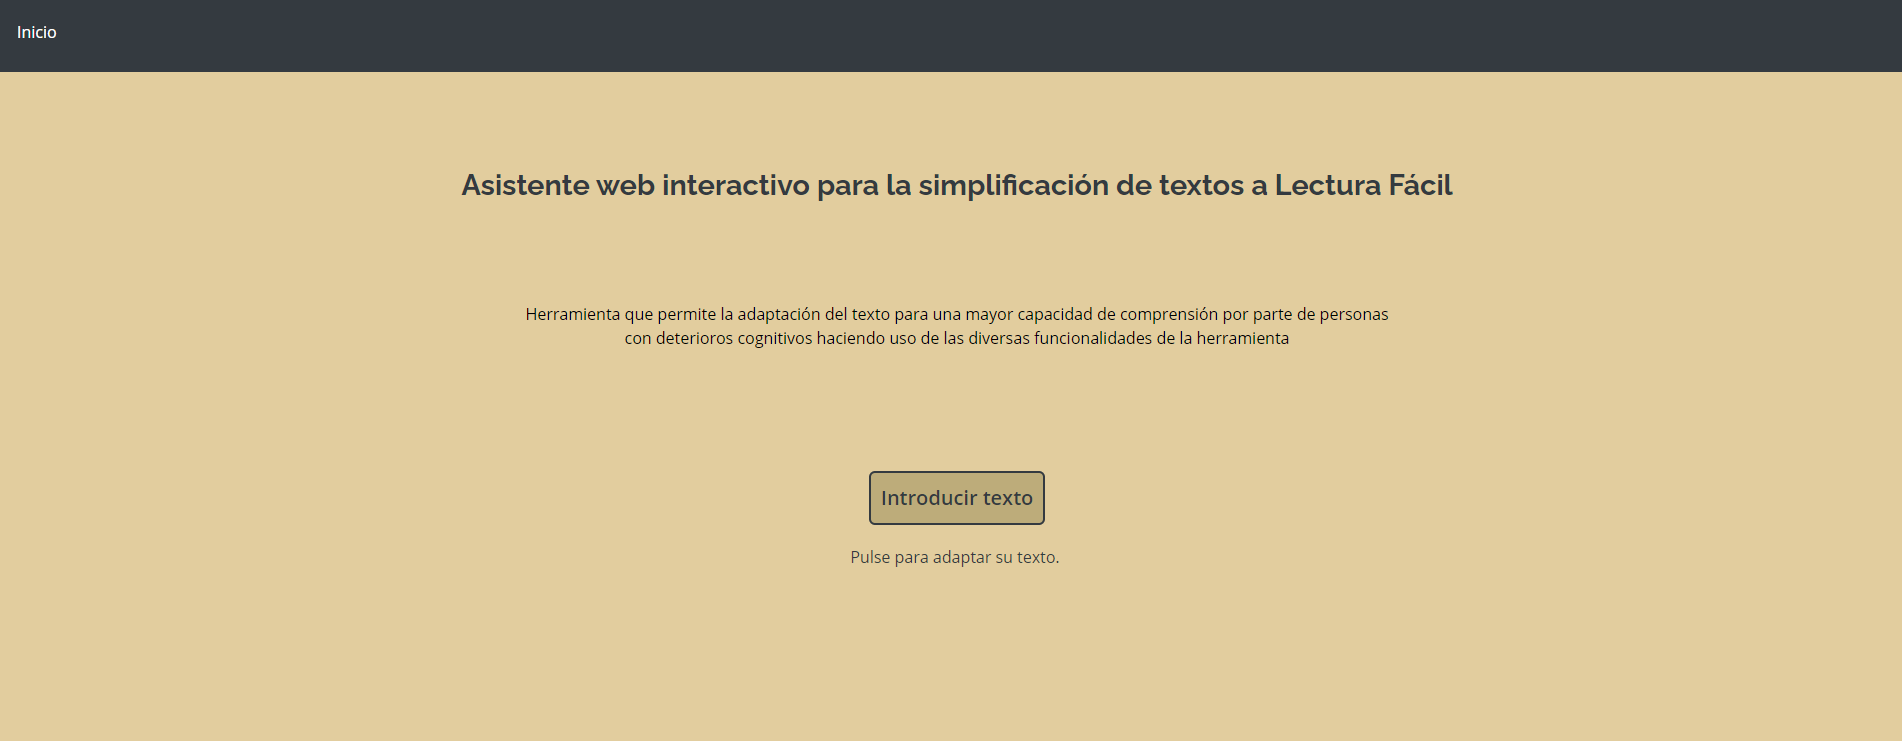
\includegraphics[scale=1]{Imagenes/Figuras/InterfazInicial}
 	
 	
 	\caption{Interfaz inicial del asistente.}
 	\label{fig:interfazInicial}
 \end{figure}
 
 Al pulsar en dicho botón se mostrará un panel lateral con las siguientes opciones:
 
 \begin{itemize}
 	\item \textbf{Texto original}: un  panel donde se introducirá el texto que queremos adaptar (ver Figura \ref{fig:interfazIntroduccionTexto}).
 	\begin{figure}[h!]
 		\centering
 		
 		
 		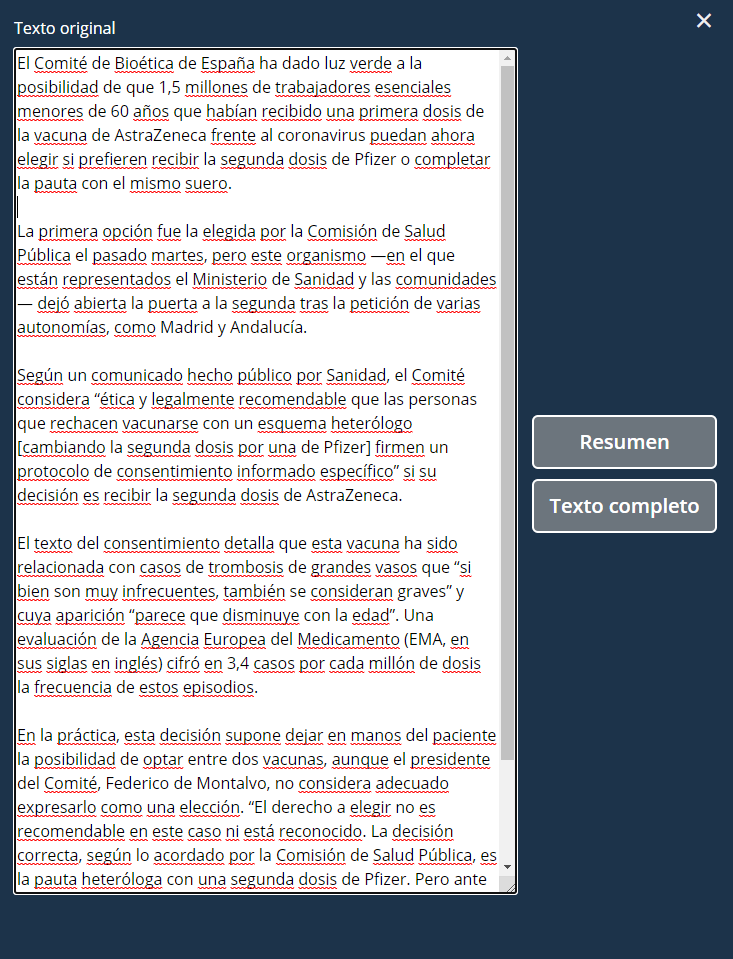
\includegraphics[scale=0.7]{Imagenes/Figuras/PanelIzquierdo}
 		
 		
 		\caption{Introducción de texto.}
 		\label{fig:interfazIntroduccionTexto}
 	\end{figure}
 	 	\item \textbf{Botón (Resumen)}: si pulsamos esta opción se mostrará una vista con una serie de frases seleccionables partiendo del resumen del texto original previamente introducido (véase Figura \ref{fig:interfazFraseTextoResumido}). Este botón permanecerá inactivo hasta que se introduzca texto. 
 	 	 	\item \textbf{Botón (Texto completo)}: si, por el contrario, pulsamos esta opción se mostrará el texto completo dividido en frases, también seleccionables (Figura \ref{fig:interfazIntroducirCompleto}). Al igual que el anterior botón también permanecerá inactivo hasta que el usuario introduzca texto. 
 	 	 \begin{figure}[h!]
 	 	 	\centering
 	 	 	
 	 	 	
 	 	 	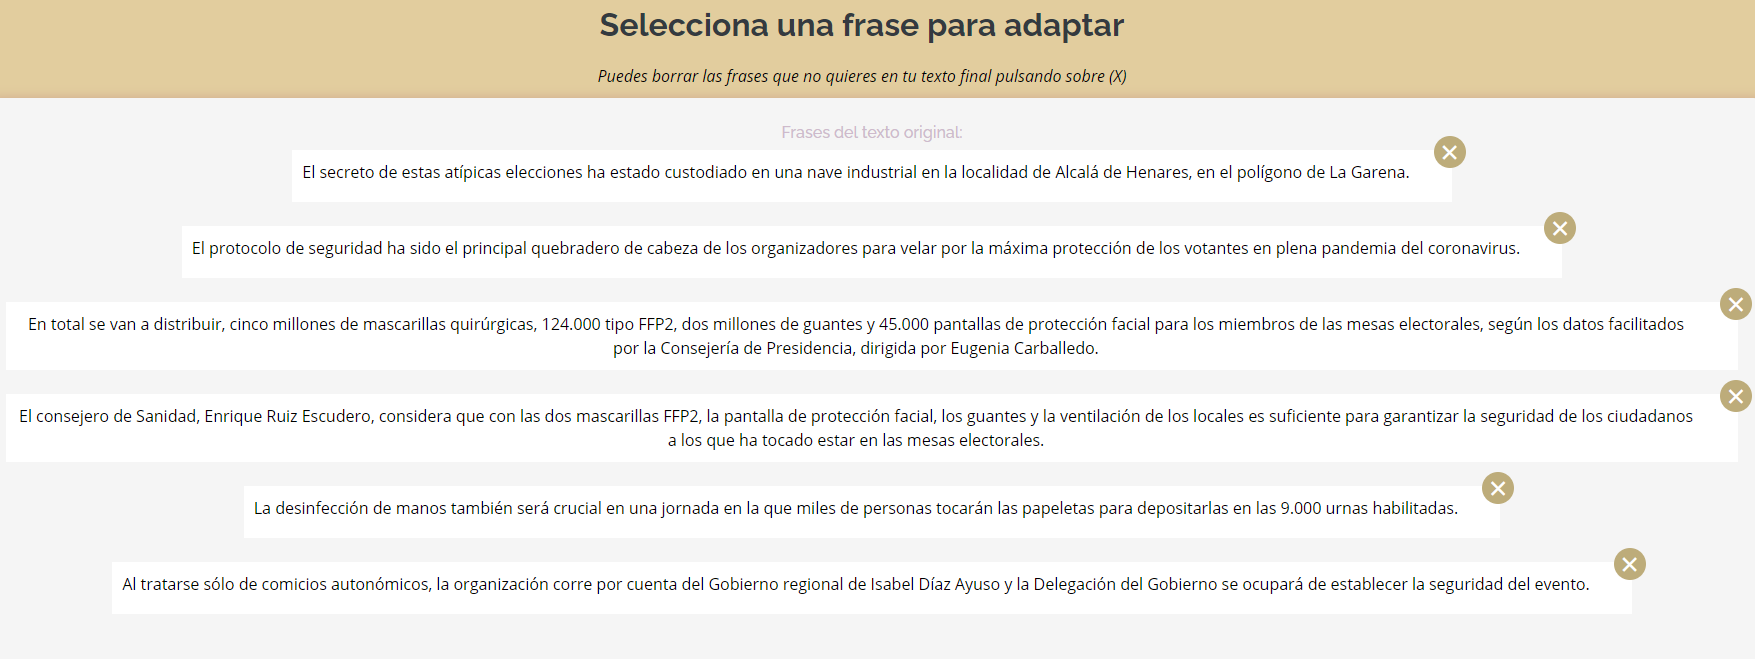
\includegraphics[scale=0.7]{Imagenes/Figuras/Resumen}
 	 	 	
 	 	 	
 	 	 	\caption{Frases partiendo del resumen.}
 	 	 	\label{fig:interfazFraseTextoResumido}
 	 	 \end{figure}
 	 	 
 	 	 
 	 	 \begin{figure}[h!]
 	 	 	\centering
 	 	 	
 	 	 	
 	 	 	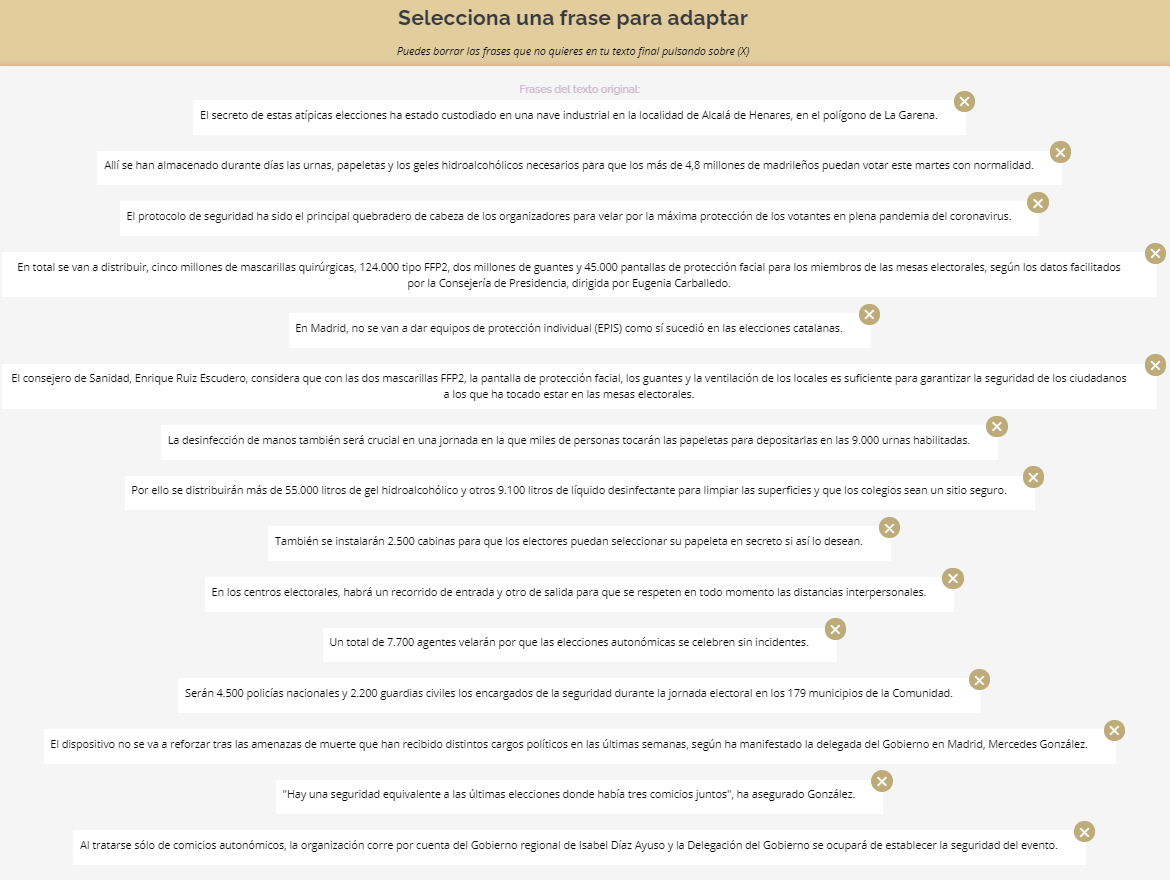
\includegraphics[scale=0.7]{Imagenes/Figuras/TextoCompleto}
 	 	 	
 	 	 	
 	 	 	\caption{Frases partiendo del texto completo.}
 	 	 	\label{fig:interfazIntroducirCompleto}
 	 	 \end{figure}	
 \end{itemize}

	Recordemos que en la Figura \ref{fig:interfazInicial} sólo contábamos con la pestaña de ``Inicio'' en la barra de navegación, la cuál cambia añadiendo una nueva pestaña \textbf{``Texto original''}. Esta pestaña nos permitirá consultar siempre el texto original que hemos introducido y cambiar en cualquier punto del flujo la opción elegida detallada anteriormente (resumen o texto completo). 


\section{Adaptaciones sobre frases}

Al clicar  sobre una frase se cambiará a una vista donde aparecerá el árbol de dependencias (véase Figura \ref{fig:arbolDependencias}), que describe la estructura sintáctica de dicha frase, que le servirá al editor a la hora de adaptarla de una manera interactiva. 

En dicho árbol encontramos las unidades léxicas separadas de la frase, las cuales podremos pulsar y realizar una serie de operaciones (botones) que se encuentran en la parte inferior izquierda. Junto a estos, aparece una breve explicación de la funcionalidad (ver operaciones que podemos efectuar en la Figura \ref{fig:botonesFuncionales}) que detallaremos en el capitulo XX. 

En la parte superior de la pantalla el editor podrá visualizar en todo momento la frase previamente elegida y un enlace (\textbf{Volver a las frases}) para volver al listado de frases, en el caso de que se quiera elegir otra o retomar alguna que ya haya sido modificada.

 En la parte inferior derecha de la vista, tenemos el borrador del texto final (Ver Figura \ref{fig:borradorTextoFinal}) donde se puede visualizar la transformación de la frase seleccionada (en negrita) habiendo realizado, o no, las diferentes operaciones. 
\begin{figure}[h!]
	\centering	
	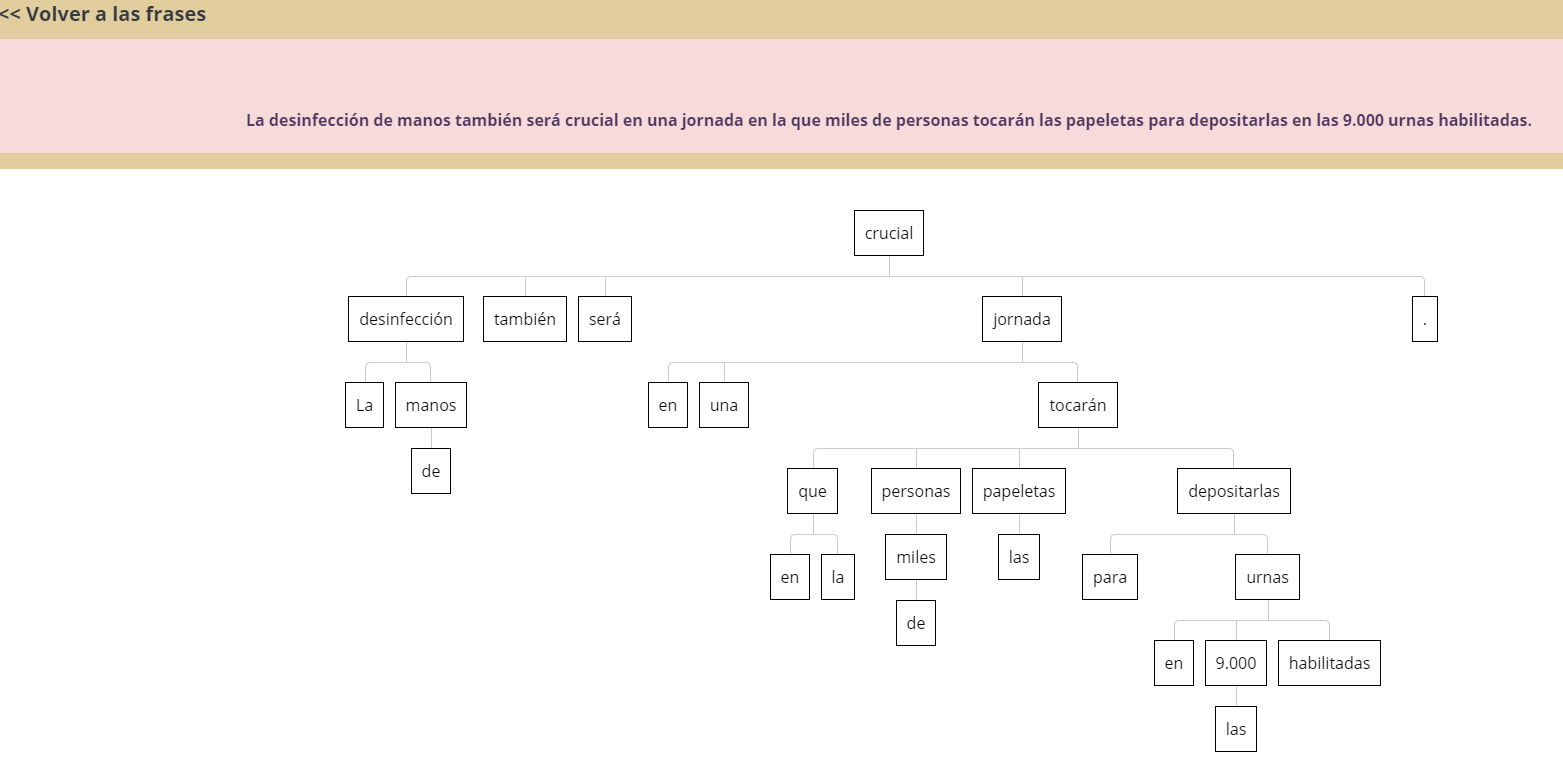
\includegraphics[scale=0.7]{Imagenes/Figuras/arbol}	
	\caption{Árbol de dependencias.}
	\label{fig:arbolDependencias}
\end{figure}
\begin{figure}[h!]
	\centering
	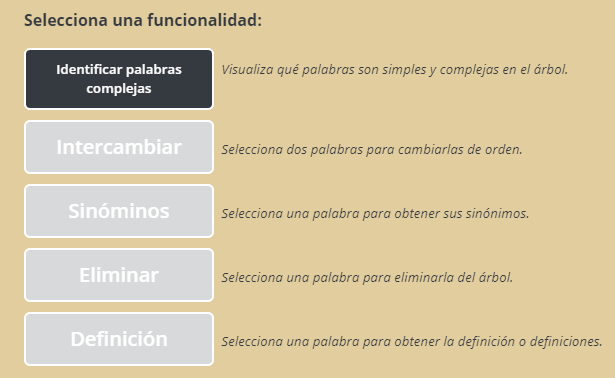
\includegraphics[scale=1.0]{Imagenes/Figuras/botonesFuncionales}
	\caption{Operaciones que podemos efectuar en el árbol de dependencias}
	\label{fig:botonesFuncionales}
\end{figure}
\begin{figure}[h!]
	\centering
	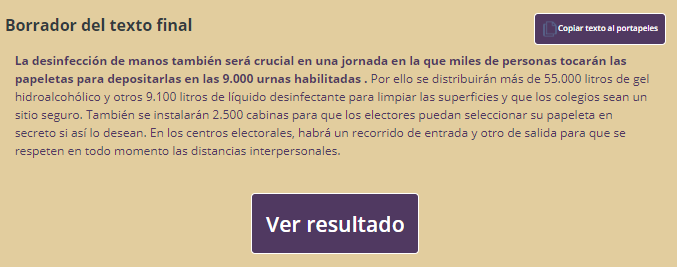
\includegraphics[scale=1.0]{Imagenes/Figuras/borradorTextoFinal}
	\caption{Borrador del texto final.}
	\label{fig:borradorTextoFinal}
\end{figure}


A continuación, describiremos en qué consisten, en qué situaciones y cómo el usuario debe utilizar cada una de las operaciones que se pueden efectuar.

\subsection{Palabras complejas}
Esta funcionalidad es de utilidad cuando el editor desee conocer aquellos términos de la frase que pueden ser susceptibles de ser reemplazados por sinónimos que sean más asequibles de comprender para el lector. El elemento visual que se encargará de esta función es el botón \textbf{Identificar palabras complejas}.

Una vez hagamos clic en este botón nuestro árbol de dependencias mostrará las palabras complejas. Como podemos ver en la Figura \ref{fig:palabrasComplejas}, aparece una leyenda en la parte superior izquierda del árbol, indicando el color en el que se colorean las complejas. Una vez pulsado, el texto del botón cambiará a \textbf{Desactivar palabras complejas} para poder volver a la vista original del árbol de dependencias.  
	 \begin{figure}[h!]
	\centering
	
	
	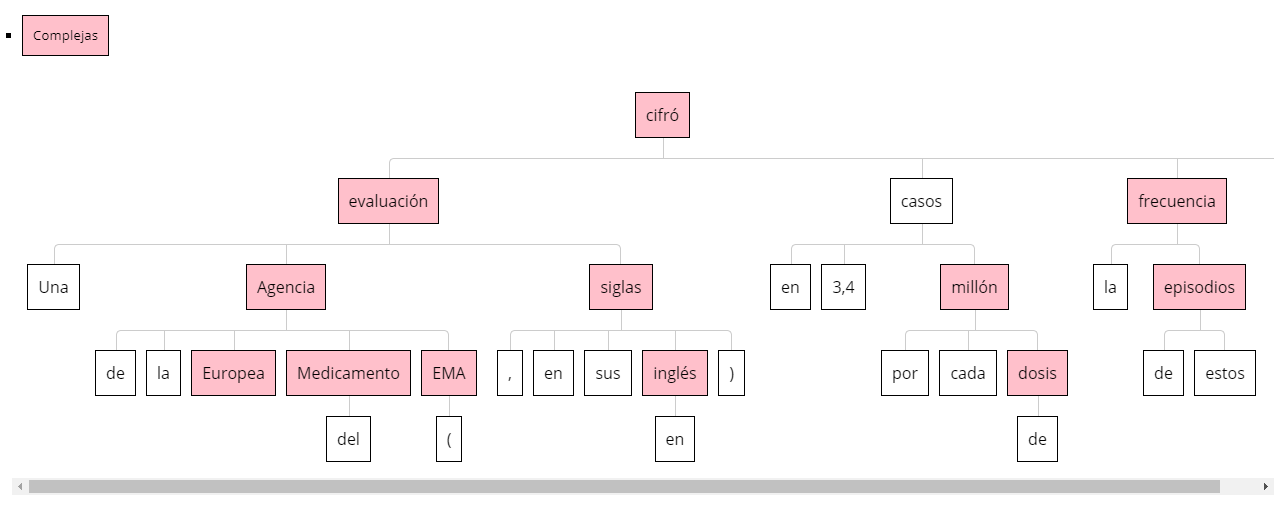
\includegraphics[scale=0.7]{Imagenes/Figuras/palabrasComplejas}
	
	
	\caption{Palabras complejas resaltadas en el árbol.}
	\label{fig:palabrasComplejas}
\end{figure}
\subsection{Intercambio de partes en el árbol de dependencias}
En caso de que el editor desee modificar el orden sintáctico de la frase, por ejemplo, se puede dar la situación de que la segunda parte de una frase sea más importante y por ende se quiera que el lector ponga más atención a esa parte. 

Para que esta funcionalidad se active es necesaria tener seleccionadas dos palabras del árbol. Ambas palabras cambiarán de orden incluyendo también aquellas que dependan de la misma (intercambio de dos palabras en el árbol de dependencias en las Figuras \ref{fig:eleccionIntercambio} y \ref{fig:intercambio}). El texto resultante quedaría como se muestra en la Figura \ref{fig:borradorIntercambio}
\begin{figure}[h!]
	\centering
	
	
	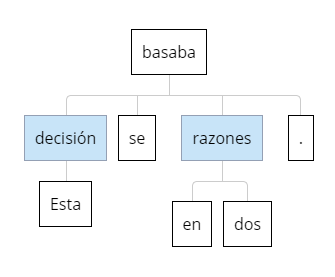
\includegraphics[scale=1]{Imagenes/Figuras/EleccionIntercambio}
	
	
	\caption{Elección de dos palabras para el intercambio.}
	\label{fig:eleccionIntercambio}
\end{figure}
\begin{figure}[h!]
	\centering
	
	
	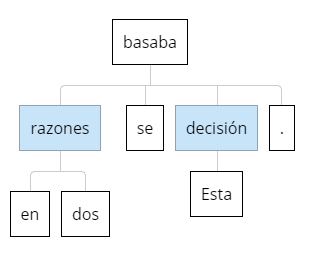
\includegraphics[scale=1]{Imagenes/Figuras/IntercambioArbol}
	
	
	\caption{Árbol de dependencias después del intercambio.}
	\label{fig:intercambio}
\end{figure}
\begin{figure}[h!]
	\centering
	
	
	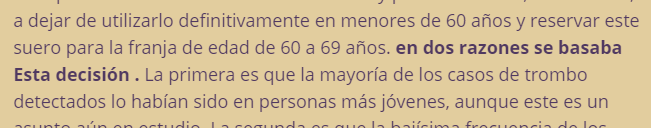
\includegraphics[scale=1]{Imagenes/Figuras/BorradorIntercambio}
	
	
	\caption{Resultado en el borrador del texto final tras el intercambio.}
	\label{fig:borradorIntercambio}
\end{figure}
\subsection{Sinónimos}
En ocasiones el usuario se verá en la necesidad de realizar una simplificación léxica sustituyendo una palabra por un sinónimo más conocido. Podrá hacer uso de ella, pulsando sobre el botón (\textbf{Sinónimos}), siempre y cuando se haya seleccionado una palabra del árbol previamente. Una vez pulsado, se muestra, si los tiene, todos los sinónimos de la palabra elegida. En caso de que la palabra no tenga sinónimos aparecerá un texto informando que carece de ellos. Si los tiene, se mostrará un listado de estos indicando cuáles son sencillos y cuáles no (ver opción sinónimos en la Figura \ref{fig:listaSinonimos}).

	 \begin{figure}[h!]
	\centering
	
	
	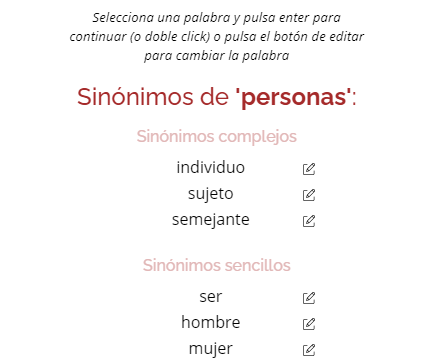
\includegraphics[scale=1.0]{Imagenes/Figuras/SinonimoPersona}
	
	
	\caption{Lista de sinónimos de una palabra seleccionada}
	\label{fig:listaSinonimos}
\end{figure}

 Llegados a este punto, se podrá seleccionar uno de ellos o bien haciendo doble clic o bien editándolo si fuese necesario para un significado coherente con la frase (concordancia en género, número, persona y conjugación), y posteriormente pulsar ``Enter'' para el cambio (véase la Figura \ref{fig:edicionSinonimos}).


\begin{figure}[h!]
\centering


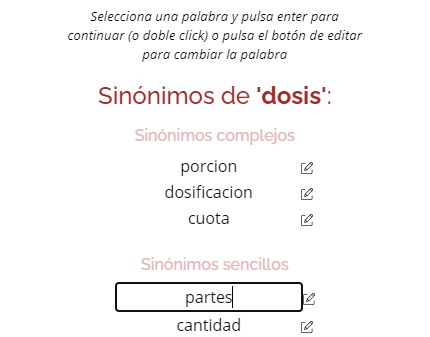
\includegraphics[scale=1.0]{Imagenes/Figuras/EditarSinonimo}


\caption{Interfaz de edición de sinónimos}
\label{fig:edicionSinonimos}
\end{figure}
Al hacer doble clic o ``Enter'', si lo hemos editado, se mostrará una ventana de diálogo (Aceptar y Cancelar) para asegurar si es realmente la acción que queremos realizar (ver Figura \ref{fig:modalSinonimos}). En el caso de que se elija ``Aceptar'', tanto en el árbol de dependencias como en el borrador del texto final se reemplazará la palabra (Figura \ref{fig:resultadoSinonimos}). En caso contrario, no habrá modificación alguna.

\begin{figure}[h!]
	\centering
	
	
	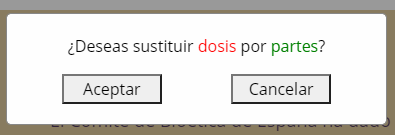
\includegraphics[scale=1.0]{Imagenes/Figuras/modalSinonimos}
	
	
	\caption{Ventana de diálogo de reemplazo de sinónimo.}
	\label{fig:modalSinonimos}
\end{figure}

\begin{figure}[h!]
	\centering
	
	
	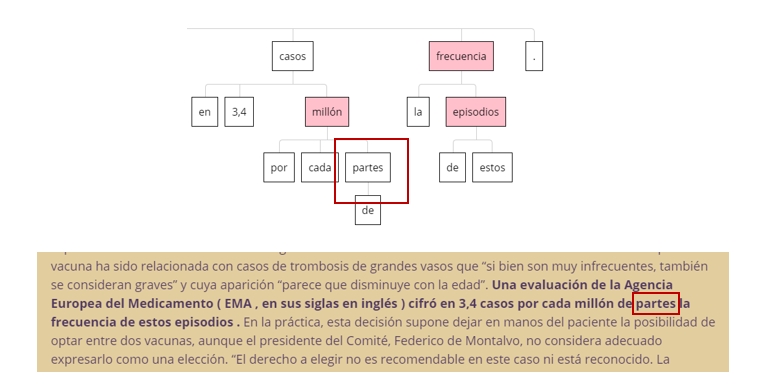
\includegraphics[scale=1.3]{Imagenes/Figuras/CambioSinonimoArbolBorrador}
	
	
	\caption{Resultado de reemplazo del sinónimo tanto en el árbol de dependencias como en el borrador}
	\label{fig:resultadoSinonimos}
\end{figure}
\subsection{Eliminar partes en el árbol de dependencias}

El editor puede encontrarse con frases que no requieren de ciertas palabras para que se capte la esencia de las mismas por parte del lector. Es por ello, por lo que tiene la opción de eliminar términos a su disposición. Es necesario seleccionar una palabra del árbol para que esta funcionalidad pueda llevarse a cabo. Suprime tanto a ella como aquellas que dependan de la misma. En las Figuras \ref{fig:eliminacionPrevia} y \ref{fig:eliminacion}, vemos la palabra seleccionada que queremos eliminar y el resultado de su eliminación en el árbol y en el texto del borrador final.
	 \begin{figure}[h!]
	\centering
	
	
	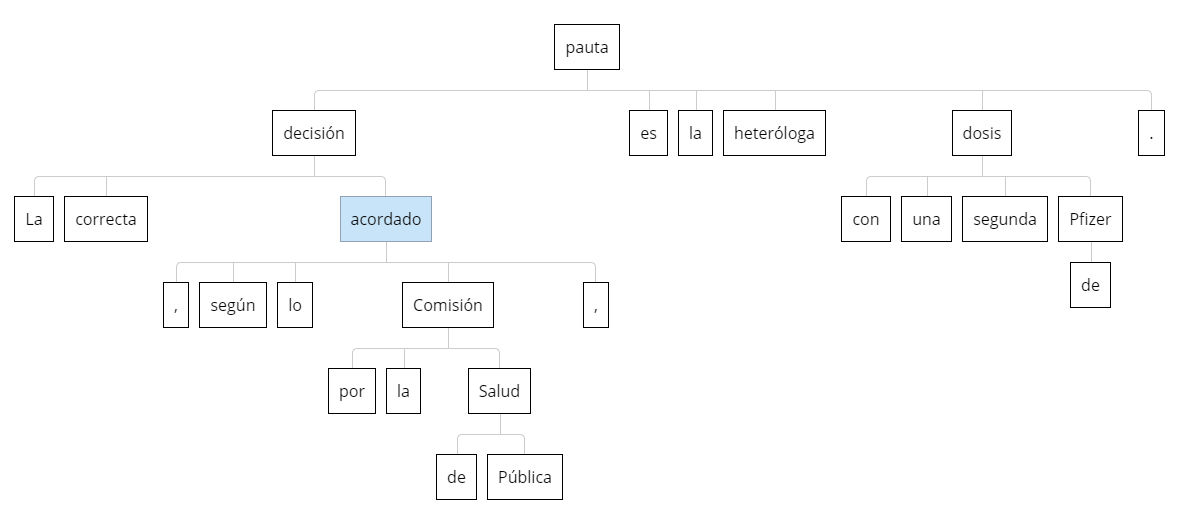
\includegraphics[scale=0.8]{Imagenes/Figuras/EleccionEliminacion}
	
	
	\caption{Árbol antes la eliminación de una palabra.}
	\label{fig:eliminacionPrevia}
\end{figure} 
	 \begin{figure}[h!]
	\centering
	
	
	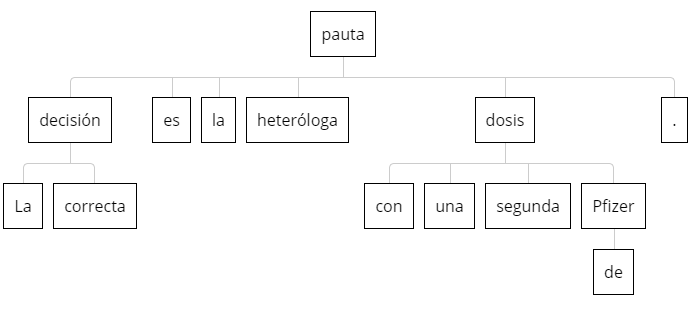
\includegraphics[scale=0.9]{Imagenes/Figuras/EliminacionSubarbol}
	
	
	\caption{Árbol tras la eliminación de una palabra.}
	\label{fig:eliminacion}
\end{figure} 
El resultado de cómo quedaría la frase lo podemos ver en la Figura \ref{fig:resultadoEliminar}.
	 \begin{figure}[h!]
	\centering
	
	
	\includegraphics[scale=1]{Imagenes/Figuras/BorradorEliminacion}
	
	
	\caption{Borrador del texto final tras la eliminación de una palabra.}
	\label{fig:resultadoEliminar}
\end{figure} 

\subsection{Definiciones respecto a una palabra}
 Gracias a esta funcionalidad, el usuario podrá nutrir el texto final con definiciones de uno o varios términos. 
 
 Seleccionando una palabra en el árbol, el botón (\textbf{Definición}) se activará. Al pulsar sobre este se mostrará un listado con todas las acepciones, si las tiene, de la palabra seleccionada (Figura \ref{fig:definiciones}). Haciendo clic en una de ellas, ésta se adjuntará a modo glosario como parte del texto final, sirviendo de apoyo a la comprensión del mismo (ver Figura \ref{fig:definicionesBorrador}). En caso de que no posea definiciones (por ejemplo, nombres propios) aparecerá un texto informando que carece de ellas.
 	 \begin{figure}[h!]
 	\centering
 	
 	
 	\includegraphics[scale=0.8]{Imagenes/Figuras/DefinicionesPersonas}
 	
 	
 	\caption{Listado de las definiciones}
 	\label{fig:definiciones}
 \end{figure}
 	 \begin{figure}[h!]
	\centering
	
	
	\includegraphics[scale=0.8]{Imagenes/Figuras/GlosarioBorrador}
	
	
	\caption{Glosario adjunto al borrador del texto final.}
	\label{fig:definicionesBorrador}
\end{figure}
\subsection{Resultado de la adaptación}
 
Cuando hayamos considerado que el texto esté adaptado a nuestras necesidades, podemos visualizarlo haciendo clic en el botón (\textbf{Ver resultado}), el cuál lo encontramos en la parte inferior derecha del borrador del texto final (ver Figura \ref{fig:botonResultado}). Al pulsarlo, desplegará un panel, el cual es editable, en la parte derecha con el mismo texto que obtuvimos en el borrador (este panel lo podemos ver en la Figura \ref{fig:panelFinal}). Esto es útil, por ejemplo, si el editor desea incluir el glosario dentro del contexto de las frases (Figura \ref{fig:}). 
\begin{figure}[h!]
	\centering
	
	
	\includegraphics[scale=0.8]{Imagenes/Figuras/verResultado}
	
	
	\caption{Botón Ver resultado junto al borrador del texto final.}
	\label{fig:botonResultado}
\end{figure}
\begin{figure}[h!]
	\centering
	
	
	\includegraphics[scale=0.8]{Imagenes/Figuras/PanelDerecho}
	
	
	\caption{Panel con el resultado final del texto adaptado}
	\label{fig:panelFinal}
\end{figure}

Como hemos visto en la Figura \ref{fig:botonResultado}, también contamos con un botón (\textbf{Copiar al portapapeles}) que nos da la opción de copiar el texto del borrador para poder introducirlo en cualquier herramienta externa.



\chapter{Implementación}
\label{cap:implementacion}

\chapterquote{Puede que tengas grandes ideas en la cabeza, pero lo que importa es la acción. Una idea, si no se lleva a cabo, no producirá ninguna manifestación, ni resultados ni recompensas}{Miguel Ruiz}


En este capítulo hacemos una descripción detallada sobre la arquitectura en la que está basada nuestro asistente. Hablaremos también sobre la implementación de las distintas funcionalidades (ver sección XXXX) que se ha llevado a cabo tanto en la parte Back End como Front End.


\section{Arquitectura}

La estructura de nuestro proyecto está soportado sobre un entorno Flask, teniendo el nivel de directorios que se muestra en la Figura \ref{fig:projectStructure}.

	 \begin{figure}[h!]
	\centering
	
	
	\includegraphics[scale=1.2]{Imagenes/Figuras/Project-Structure}
	
	
	\caption{Estructura del proyecto en Flask}
	\label{fig:projectStructure}
\end{figure}

A continuación, se explican la función de cada uno de los ficheros que componen la aplicación web.

\subsection{Ficheros del entorno}

Los ficheros principales son:
\begin{itemize}
	\item \textbf{views.py}: es el encargado de la lógica de todos los endpoints de la aplicación, así como el renderizado de la plantilla. Cada uno de esos endpoints tendrá una funcionalidad distinta, los cuales serán llamados por una función de funciones.js 
	\item \textbf{vo.py}: se encarga de la organización de clases.
	\item \textbf{home.html}: en este archivo creamos la estructura de nuestro asistente y la organización que mostrará el contenido.
	\item \textbf{funciones.js}: la misión de este fichero es comunicar la aplicación web con los elementos del DOM de la misma, haciendo posible la modificación del HTML dinámicamente. Las modificaciones que efectuamos en este archivo es añadir nuevas etiquetas, modificando o eliminando otras, cambiar sus atributos, añadiendo clases, cambiar el contenido de texto, etc. También es el encargado de la comunicación con la vista (views.py) para la petición y respuesta de servicios web.
	\item \textbf{arbol.css}: archivo encargado de generar los estilos para que nuestro árbol de dependencias tenga la apariencia de un árbol genealógico.
	\item \textbf{style.css}: fichero encargado de dar estilos a todo lo que concierne nuestra aplicación web excepto el árbol de dependencias (fuentes, disposición, tamaños, colores, etc.)   
\end{itemize}

\subsection{Servicios web externos}\label{sec:serviciosWebExternos}
Para hacer uso de las principales funcionalidades descritas en la sección XXX, contamos con una arquitectura de servicios web REST basada en endpoints (URLs), intercambiando mensajes entre cliente y servidor (Figura \ref{fig:apiRest}). 

\begin{figure}[h!]
	\centering
	
	
	\includegraphics[scale=0.4]{Imagenes/Figuras/rest_api}
	
	
	\caption{Servicio REST cliente/servidor}
	\label{fig:apiRest}
\end{figure}

Un servicio web REST es una interfaz para conectar varios servicios web basados en el protocolo HTTP que define una gran cantidad de métodos, de los cuales describimos los cuatro más básicos:
\begin{itemize}
	\item \textbf{GET}: se utiliza para acceder a los distintos recursos. Si requiere del envío de un parámetro al servidor (URI param), éste se pasa como un elemento en la URI (del inglés, \textit{Uniform Resource Identifier}). 
	
	\item \textbf{POST}: se usa para realizar acciones de creación de nuevos recursos. Si se requiere el envío de información al servidor, esta se pasa dentro del cuerpo de la petición HTTP (body param).
	
	\item \textbf{PUT}: se utiliza para la modificación de los recursos existentes. Puede enviar parámetros tanto en la URI como en el cuerpo de la petición HTTP.
	
	\item \textbf{DELETE}: se utiliza para la eliminar los recursos existentes, siendo la operación análoga al POST. El parámetro será informado a través de la URI.
\end{itemize}

Estas métodos pueden ser usados en distintas situaciones devolviendo los datos en distintos formatos como XML y JSON.
En nuestro caso, hemos usado el formato JSON.

Nuestra arquitectura REST tiene el aspecto como muestra la Figura \ref{fig:ArquitecturaAsistenteR}, que a continuación describimos.
\begin{figure}[h!]
	\centering
	
	
	\includegraphics[scale=0.9]{Imagenes/Figuras/ArquitecturaAsistenteR}
	
	
	\caption{Diagrama de la arquitectura REST del asistente web}
	\label{fig:ArquitecturaAsistenteR}
\end{figure}

  Hacemos uso de los siguientes servicios REST que nos ofrece la API del grupo NIL\footnote{Para más información acceder a \href{https://holstein.fdi.ucm.es/nil-ws-api/}{https://holstein.fdi.ucm.es/nil-ws-api/}} (descrita en el capítulo X sección XXX):


	


\begin{itemize}
	\item \textbf{Servicio para comprobar si una palabra es compleja}.
	\begin{lstlisting}[backgroundcolor = \color{pink},
	xleftmargin = 1cm,
	framexleftmargin = 1em,frame=tlbr,framesep=4pt,framerule=1pt]
	GET https://holstein.fdi.ucm.es/nil-ws-api/palabra/
	{palabra}/es\_sencilla
	
	
\end{lstlisting}
	
	Este recurso devuelve un objeto en formato JSON que contiene el campo ``palabraSencilla'' de tipo booleano que en el caso que sea False la palabra introducida a través de la URI es compleja (ver Figura \ref{fig:apiSencilla}).
		 \begin{figure}[h!]
		\centering
		
		
		\includegraphics[scale=1]{Imagenes/Figuras/APISencilla}
		
		
		\caption{Petición para comprobar si una palabra es compleja}
		\label{fig:apiSencilla}
	\end{figure}
	\item \textbf{Servicio para obtener definiciones de una palabra}.
\newline

	\begin{lstlisting}[backgroundcolor = \color{pink},
	xleftmargin = 1cm,
	framexleftmargin = 1em,frame=tlbr,framesep=4pt,framerule=1pt]
	GET https://holstein.fdi.ucm.es/nil-ws-api/palabra/
	{palabra}/definiciones

	
	
\end{lstlisting}




En este caso, el servicio devuelve un objeto JSON que contiene el campo ``definiciones'' de tipo arrayList en el que en cada posición hay otro objeto, ``definicion'', cuyo valor es de tipo string con la acepción correspondiente (ver Figura \ref{fig:apiDefinicion}).
\begin{figure}[h!]
	\centering
	
	
	\includegraphics[scale=1]{Imagenes/Figuras/ApiDefinicion}
	
	
	\caption{Petición que devuelve una lista de definiciones}
	\label{fig:apiDefinicion}
\end{figure}
	\item \textbf{Servicio para obtener sinónimos de una palabra}.
	\begin{lstlisting}[backgroundcolor = \color{pink},
	xleftmargin = 1cm,
	framexleftmargin = 1em,frame=tlbr,framesep=4pt,framerule=1pt]
	GET https://holstein.fdi.ucm.es/nil-ws-api/palabra/
	{palabra}/sinonimos	
	
	
	
	
\end{lstlisting}



El servicio devuelve un objeto JSON que contiene el campo ``sinonimos'' de tipo arrayList en el que en cada posición hay otro objeto, ``sinonimo'', cuyo valor es de tipo string con la acepción correspondiente (ver Figura \ref{fig:apiSinonimo}).
\begin{figure}[h!]
	\centering
	
	
	\includegraphics[scale=1]{Imagenes/Figuras/APISinonimos}
	
	
	\caption{Petición que devuelve una lista de sinónimos}
	\label{fig:apiSinonimo}
\end{figure}
\end{itemize}

Cabe destacar que esta API no hace uso de las reglas de acentuación, de manera que debemos de insertar las palabras sin tildes (obsérvese la Figura \ref{fig:apiSinonimo}).

\subsection{Librería Spacy}

\subsection{Implementaciones del servidor}

\subsection{Implementaciones de la aplicación web}

En esta sección se explica en detalle como han sido desarrolladas las funcionalidades (capítulo \ref{cap:asistenteWeb} \ref{sec:}) de la aplicación web, cuya finalidad es proporcionar al usuario una interfaz sencilla, donde puedan introducir un texto, hacer una serie de transformaciones para obtener el mismo simplificado a Lectura Fácil.


Para que el contenido de la aplicación web sea dinámico se ha desarrolla con JavaScript, cambiando según la acción del usuario. Estás acciones son:

\begin{itemize}
	\item Botón (\textbf{Resumen}): se realiza una llamada Fetch al endpoint ``/summary'' con el texto completo previamente introducido. La respuesta recibida será un objeto JSON, el cuál contiene el resumen del texto. Posteriormente se hará otra llamada Fetch al endpoint ``/sentences'', que devuelve el texto en frases. Estás frases se incrustan en el código HTML, escribiéndolas a modo de lista (una debajo de otra).    
 
	\item Botón (\textbf{Texto completo}): a diferencia de botón anterior este hace una llamada únicamente al endpoint ``/sentences'', devolviendo el texto completo en frases.

	\item Creación del árbol de dependencias: se realiza una llamada Fetch al endpoint ``/sentences/tree'', devolviendo así un objeto JSON con la estructura del árbol. Para su construcción de este, hemos usado un algoritmo de búsqueda en profundidad (BFS), recorriendo todos los nodos (en nuestro caso palabras de la frase). El funcionamiento de este algoritmo consiste en ir expandiendo cada uno de sus nodos desde la raíz hacia el nodo hoja (no tiene más hijos) de manera recurrente (Figura \ref{fig:diagramaBFS}).
	\begin{figure}[h!]
		\centering
		
		
		\includegraphics[scale=1]{Imagenes/Figuras/diagramaBFS}
		
		
		\caption{Petición que devuelve una lista de sinónimos}
		\label{fig:diagramaBFS}
	\end{figure}
	
		Por ejemplo, supongamos que queramos adaptar la frase ``También se instalarán 2.500 cabinas para que los electores puedan seleccionar su papeleta en secreto si así lo desean.'', el objeto JSON tendría el aspecto de la Figura \ref{fig:objetoJSON}. 
	Cada nodo contiene los siguientes datos:
		\begin{itemize}
		\item \textbf{children}: array de nodos hijos.
		\item \textbf{height}: nivel del nodo con respecto a la raíz (en nuestro ejemplo ``instalarán'' sería nuestra raíz, que tiene una altura 0).
		\item \textbf{id}: identificador único de cada nodo.
		\item \textbf{text}: palabra propia del nodo.
	\end{itemize}
En la Figura \ref{fig:arbolDependencias} observamos el árbol con el que podremos interactuar durante la adaptación.
	\item Palabras complejas.
	\item 
\end{itemiz
%\include{Capitulos/Capitulo5}
\chapter{Conclusiones y Trabajo Futuro}
\label{cap:conclusiones}

Conclusiones del trabajo y líneas de trabajo futuro.



\chapter{Trabajo individual}
\label{cap:trabajoIndividual}

\section{Estefanía Ortega Ávila}

En primer lugar, mi labor en este TFG se centró en una investigación de las tareas y los pasos a seguir que se llevan a cabo para adaptar un texto a Lectura Fácil. Para ello, consulté diversas webs y vídeos que me proporcionaran dicha información. De esta manera, entendí a qué público iba dirigida este tipo de lectura y qué técnicas eran las más utilizadas. 

Posteriormente, tanto mi compañero como yo, identificamos diferentes herramientas que podrían ser útiles para transformar textos, probando algunas de ellas, haciéndonos una idea de qué medios disponen los editores para realizar su labor.

Una vez realizada la investigación, mi compañero y yo comenzamos a estudiar las tecnologías que iban a hacer posible la implementación de nuestro asistente web. Optamos por hacer uso de servicios API REST, así como de la librería spaCy para el PLN.

Por otro lado, y esta es la que yo abordé, tenemos la implementación de la aplicación, es decir, la interfaz visual con el que el usuario editor interactuará y hará uso de las diferentes funcionalidades. 

Para el desarrollo de esta implementación, utilicé JavaScript para que los resultados de la llamada al servidor mediante una promesa Fetch a un endpoint me devolviera un objeto JSON que, al operar sobre él, plasme cierta información en la interfaz; usando HTML, para el desarrollo de la interfaz visual, y CSS para dar estilo a ésta (fuentes, tamaños, colores…).


La parte donde tuve más dificultad fue la de dibujar el árbol de dependencias con el aspecto de árbol genealógico y el poder procesar el objeto JSON que recibo del servidor para representar cada nodo con sus correspondientes dependencias. La solución por la que opté fue la de implementar un algoritmo BFS para poder recorrer el objeto, obteniendo la estructura de árbol deseada.

Otra parte de especial dificultad fue la relacionada con la funcionalidad ``Intercambiar'' en el caso de que se tuviera que modificar dos palabras independientes entre sí y, a su vez, las dependientes de éstas, reflejándose estos cambios en el borrador del texto final. Para solventarlo, hice uso de arrays auxiliares que me permitieron obtener el resultado que quería en el borrador para poder cambiar el texto dinámicamente.

Realicé algunas pruebas en Postman de los diferentes servicios de NIL-WS-API para validar que el comportamiento de la interfaz, se correspondía con lo que la API devolvía en su respuesta, por ejemplo, en el caso de comprobar que si una palabra se muestra de color rojo en el árbol, la API nos indique que dicha palabra es compleja. Esto me permitió, por primera vez, hacer uso de la herramienta Postman, la cual es bastante apropiada para el testeo de APIs.

Para el diseño de la interfaz del asistente, tomé en cuenta las recomendaciones de mis tutoras en las reuniones periódicas, sobre todo en lo que concierne a nombres de botones, elementos de la interfaz visibles o no visibles al pinchar en una determinada funcionalidad, etc.



Además de la implementación, me encargué de algunas de las partes que consta la memoria. En el capítulo 1, redacté los puntos relacionados con la motivación y los objetivos que persigue este asistente. El capítulo 2, los puntos 2.3 y 2.4 relacionados con proyectos, programas y aplicaciones en LF. Con respecto al capítulo 4, fui la persona encargada de desarrollarlo en su totalidad hablando sobre la aplicación y sus diferentes funcionalidades y vistas, mientras que del capítulo 5 fui la autora del punto 5.1 y 5.3, relacionados con la arquitectura y con la implementación del asistente, respectivamente. Finalmente, el capítulo 6, lo elaboré junto con la ayuda de mi compañero. Por último, traduje al inglés la parte de mi trabajo individual.



Por supuesto, se fue realizando modificaciones en aquellas partes que a nuestras tutoras les parecía que debíamos mejorar.

\section{Javier Sesé García}

Mi contribución al proyecto comenzó investigando a quién iba dirigida la Lectura Fácil y las formas que se utilizaban para adaptar textos. 

Posteriormente, nos centramos en el diseño de la arquitectura de la aplicación, la cual es una arquitectura REST basada en endpoints. Elegimos este diseño ya que nos pareció que es fácilmente ampliable en el caso de que se quisiera realizar un servicio nuevo.

Implementé esta arquitectura con Flask, del cual he adquirido los conocimientos para ser capaz de desplegar el servidor en él. He elegido Flask ya que, aunque tenía más experiencia con Django, me ha parecido un entorno ligero y fácil de usar y una oportunidad de ampliar mis conocimientos.

En lo que concierne a las herramientas, investigué y aprendí a usar la librería spaCy que otorga la principal funcionalidad de análisis gramatical del asistente. Para ello tuve que familiarizarme con todas las funcionalidades de spaCy que hemos usado, investigando en profundidad lo que podían hacer y de qué manera, así como hacer un repaso de la gramática, para entender completamente el funcionamiento y uso que le podemos dar a la funcionalidad del etiquetado gramatical de spaCy.


Además, implementé las llamadas a los diferentes servicios de NIL-WS-API desde la parte del servidor, escrito con lenguaje Python.

Al igual que mi compañera, me serví de Postman para verificar los datos que recibía el servidor, y gracias a ello encontré una carencia de la API, y es que no acepta caracteres especiales, ya que estos se pasan como argumento de la URI, por lo que decidí, como posible solución, eliminar estos caracteres de las palabras.

 Por el contrario, esta solución presentaba otro problema en sí, y es que sin esos caracteres especiales se da ambigüedad en los resultados de los servicios, como por ejemplo el de sinónimos, que la propia API ya considera retornando todos los posibles valores, por lo que decidimos hacer lo mismo y dejar a elección del usuario el valor con el que quedarse.

Desconocía como se debían de hacer las llamadas a los endpoints del servidor, lo que me supuso un esfuerzo hasta que aprendí a realizar las promesas mediante la operación Fetch. Adicionalmente, implementé parte de la funcionalidad de las propias promesas en JavaScript junto con mi compañera.

También investigué como hacer la conjugación de palabras a partir de su lema, tiempo verbal y número gramatical, lo que me llevó a la conclusión de que no sería capaz de hacerlo solamente con spaCy, por lo que busqué otras formas de realizarlo en Python. 

Llegué a dar con varias formas de realizar esta conjugación, pero ninguna adaptada al texto en castellano a pesar de que encontré una posibilidad de montar otro servidor en Java para ello, pero valoré que no tenía el tiempo suficiente para aprender a usarlo lo cual no nos servia para esta aplicación ya que estaba disponible en inglés. 

Por otro lado, estudié la opción de hacer nuestro propio conjugador, pero de nuevo valoré que no teníamos el tiempo necesario suficiente para ello. Por todo ello, decidimos dejar la posibilidad de la conjugación automática de palabras como posible trabajo futuro. 


Una vez terminada la implementación me encargué de alojar el servidor en el contenedor que nos han otorgado (\url{https://holstein.fdi.ucm.es/tfg/2021/simpli/}). Para ello, tuve que aprender cómo usarlo, así como de saber lanzar el servidor de Flask en un docker, lo que ha obligado a realizar una modificación en las rutas de los archivos .js y .css locales.

En cuanto a la memoria además del resumen, redacté, en lo que concierne al capítulo 1, la sección de ``Estructura del documento''. En el capítulo 2  me encargué de los puntos 2.1 y 2.2. El capítulo 3 relacionados con las herramientas lo elaboré al completo. El capítulo 5 escribí las tres primeras secciones ligadas a la parte del servidor de la aplicación y la librería spaCy, salvo el punto 5.1.1. Junto con la ayuda de mi compañera, redactamos el capítulo 6 para explicar las conclusiones y posibles mejoras. Finalmente traduje la parte del resumen y palabras claves al inglés, así como mi trabajo individual.





%%%%%%%%%%%%%%%%%%%%%%%%%%%%%%%%%%%%%%%%%%%%%%%%%%%%%%%%%%%%%%%%%%%%%%%%%%%
% Si el TFM se escribe en inglés, comentar las siguientes líneas 
% porque no es necesario incluir nuevamente las Conclusiones en inglés
\setcounter{chapter}{\thechapter-1} 
\begin{otherlanguage}{english}
	\chapter{Conclusions and Future Work}
\label{cap:conclusions}

Conclusions and future lines of work.



\end{otherlanguage}
%%%%%%%%%%%%%%%%%%%%%%%%%%%%%%%%%%%%%%%%%%%%%%%%%%%%%%%%%%%%%%%%%%%%%%%%%%%


% Apéndices
\appendix
\chapter{Título}
\label{Appendix:Key1}

Contenido del apéndice
\chapter{Título}
\label{Appendix:Key2}

%\include{Apendices/appendixC}
%\include{...}
%\include{...}
%\include{...}
\backmatter

%
% Bibliografía
%
% Si el TFM se escribe en inglés, editar TeXiS/TeXiS_bib para cambiar el
% estilo de las referencias
%---------------------------------------------------------------------
%
%                      configBibliografia.tex
%
%---------------------------------------------------------------------
%
% bibliografia.tex
% Copyright 2009 Marco Antonio Gomez-Martin, Pedro Pablo Gomez-Martin
%
% This file belongs to the TeXiS manual, a LaTeX template for writting
% Thesis and other documents. The complete last TeXiS package can
% be obtained from http://gaia.fdi.ucm.es/projects/texis/
%
% Although the TeXiS template itself is distributed under the 
% conditions of the LaTeX Project Public License
% (http://www.latex-project.org/lppl.txt), the manual content
% uses the CC-BY-SA license that stays that you are free:
%
%    - to share & to copy, distribute and transmit the work
%    - to remix and to adapt the work
%
% under the following conditions:
%
%    - Attribution: you must attribute the work in the manner
%      specified by the author or licensor (but not in any way that
%      suggests that they endorse you or your use of the work).
%    - Share Alike: if you alter, transform, or build upon this
%      work, you may distribute the resulting work only under the
%      same, similar or a compatible license.
%
% The complete license is available in
% http://creativecommons.org/licenses/by-sa/3.0/legalcode
%
%---------------------------------------------------------------------
%
% Fichero  que  configura  los  parámetros  de  la  generación  de  la
% bibliografía.  Existen dos  parámetros configurables:  los ficheros
% .bib que se utilizan y la frase célebre que aparece justo antes de la
% primera referencia.
%
%---------------------------------------------------------------------


%%%%%%%%%%%%%%%%%%%%%%%%%%%%%%%%%%%%%%%%%%%%%%%%%%%%%%%%%%%%%%%%%%%%%%
% Definición de los ficheros .bib utilizados:
% \setBibFiles{<lista ficheros sin extension, separados por comas>}
% Nota:
% Es IMPORTANTE que los ficheros estén en la misma línea que
% el comando \setBibFiles. Si se desea utilizar varias líneas,
% terminarlas con una apertura de comentario.
%%%%%%%%%%%%%%%%%%%%%%%%%%%%%%%%%%%%%%%%%%%%%%%%%%%%%%%%%%%%%%%%%%%%%%
\setBibFiles{%
nuestros,latex,otros%
}

%%%%%%%%%%%%%%%%%%%%%%%%%%%%%%%%%%%%%%%%%%%%%%%%%%%%%%%%%%%%%%%%%%%%%%
% Definición de la frase célebre para el capítulo de la
% bibliografía. Dentro normalmente se querrá hacer uso del entorno
% \begin{FraseCelebre}, que contendrá a su vez otros dos entornos,
% un \begin{Frase} y un \begin{Fuente}.
%
% Nota:
% Si no se quiere cita, se puede eliminar su definición (en la
% macro setCitaBibliografia{} ).
%%%%%%%%%%%%%%%%%%%%%%%%%%%%%%%%%%%%%%%%%%%%%%%%%%%%%%%%%%%%%%%%%%%%%%
\setCitaBibliografia{
\begin{FraseCelebre}
\begin{Frase}
  Y así, del mucho leer y del poco dormir, se le secó el celebro de
  manera que vino a perder el juicio.
\end{Frase}
\begin{Fuente}
  Miguel de Cervantes Saavedra
\end{Fuente}
\end{FraseCelebre}
}

%%
%% Creamos la bibliografia
%%
\makeBib

% Variable local para emacs, para  que encuentre el fichero maestro de
% compilación y funcionen mejor algunas teclas rápidas de AucTeX

%%%
%%% Local Variables:
%%% mode: latex
%%% TeX-master: "../Tesis.tex"
%%% End:

%
% Índice de palabras
%

% Sólo  la   generamos  si  está   declarada  \generaindice.  Consulta
% TeXiS.sty para más información.

% En realidad, el soporte para la generación de índices de palabras
% en TeXiS no está documentada en el manual, porque no ha sido usada
% "en producción". Por tanto, el fichero que genera el índice
% *no* se incluye aquí (está comentado). Consulta la documentación
% en TeXiS_pream.tex para más información.
\ifx\generaindice\undefined
\else
%%---------------------------------------------------------------------
%
%                        TeXiS_indice.tex
%
%---------------------------------------------------------------------
%
% TeXiS_indice.tex
% Copyright 2009 Marco Antonio Gomez-Martin, Pedro Pablo Gomez-Martin
%
% This file belongs to TeXiS, a LaTeX template for writting
% Thesis and other documents. The complete last TeXiS package can
% be obtained from http://gaia.fdi.ucm.es/projects/texis/
%
% This work may be distributed and/or modified under the
% conditions of the LaTeX Project Public License, either version 1.3
% of this license or (at your option) any later version.
% The latest version of this license is in
%   http://www.latex-project.org/lppl.txt
% and version 1.3 or later is part of all distributions of LaTeX
% version 2005/12/01 or later.
%
% This work has the LPPL maintenance status `maintained'.
% 
% The Current Maintainers of this work are Marco Antonio Gomez-Martin
% and Pedro Pablo Gomez-Martin
%
%---------------------------------------------------------------------
%
% Contiene  los  comandos  para  generar  el índice  de  palabras  del
% documento.
%
%---------------------------------------------------------------------
%
% NOTA IMPORTANTE: el  soporte en TeXiS para el  índice de palabras es
% embrionario, y  de hecho  ni siquiera se  describe en el  manual. Se
% proporciona  una infraestructura  básica (sin  terminar)  para ello,
% pero  no ha  sido usada  "en producción".  De hecho,  a pesar  de la
% existencia de  este fichero, *no* se incluye  en Tesis.tex. Consulta
% la documentación en TeXiS_pream.tex para más información.
%
%---------------------------------------------------------------------


% Si se  va a generar  la tabla de  contenidos (el índice  habitual) y
% también vamos a  generar el índice de palabras  (ambas decisiones se
% toman en  función de  la definición  o no de  un par  de constantes,
% puedes consultar modo.tex para más información), entonces metemos en
% la tabla de contenidos una  entrada para marcar la página donde está
% el índice de palabras.

\ifx\generatoc\undefined
\else
   \addcontentsline{toc}{chapter}{\indexname}
\fi


% Generamos el índice
\printindex

% Variable local para emacs, para  que encuentre el fichero maestro de
% compilación y funcionen mejor algunas teclas rápidas de AucTeX

%%%
%%% Local Variables:
%%% mode: latex
%%% TeX-master: "./tesis.tex"
%%% End:

\fi

%
% Lista de acrónimos
%

% Sólo  lo  generamos  si  está declarada  \generaacronimos.  Consulta
% TeXiS.sty para más información.


\ifx\generaacronimos\undefined
\else
%---------------------------------------------------------------------
%
%                        TeXiS_acron.tex
%
%---------------------------------------------------------------------
%
% TeXiS_acron.tex
% Copyright 2009 Marco Antonio Gomez-Martin, Pedro Pablo Gomez-Martin
%
% This file belongs to TeXiS, a LaTeX template for writting
% Thesis and other documents. The complete last TeXiS package can
% be obtained from http://gaia.fdi.ucm.es/projects/texis/
%
% This work may be distributed and/or modified under the
% conditions of the LaTeX Project Public License, either version 1.3
% of this license or (at your option) any later version.
% The latest version of this license is in
%   http://www.latex-project.org/lppl.txt
% and version 1.3 or later is part of all distributions of LaTeX
% version 2005/12/01 or later.
%
% This work has the LPPL maintenance status `maintained'.
% 
% The Current Maintainers of this work are Marco Antonio Gomez-Martin
% and Pedro Pablo Gomez-Martin
%
%---------------------------------------------------------------------
%
% Contiene  los  comandos  para  generar  el listado de acrónimos
% documento.
%
%---------------------------------------------------------------------
%
% NOTA IMPORTANTE:  para que la  generación de acrónimos  funcione, al
% menos  debe  existir  un  acrónimo   en  el  documento.  Si  no,  la
% compilación  del   fichero  LaTeX  falla  con   un  error  "extraño"
% (indicando  que  quizá  falte  un \item).   Consulta  el  comentario
% referente al paquete glosstex en TeXiS_pream.tex.
%
%---------------------------------------------------------------------


% Redefinimos a español  el título de la lista  de acrónimos (Babel no
% lo hace por nosotros esta vez)

\def\listacronymname{Lista de acrónimos}

% Para el glosario:
% \def\glosarryname{Glosario}

% Si se  va a generar  la tabla de  contenidos (el índice  habitual) y
% también vamos a  generar la lista de acrónimos  (ambas decisiones se
% toman en  función de  la definición  o no de  un par  de constantes,
% puedes consultar config.tex  para más información), entonces metemos
% en la  tabla de contenidos una  entrada para marcar  la página donde
% está el índice de palabras.

\ifx\generatoc\undefined
\else
   \addcontentsline{toc}{chapter}{\listacronymname}
\fi


% Generamos la lista de acrónimos (en realidad el índice asociado a la
% lista "acr" de GlossTeX)

\printglosstex(acr)

% Variable local para emacs, para  que encuentre el fichero maestro de
% compilación y funcionen mejor algunas teclas rápidas de AucTeX

%%%
%%% Local Variables:
%%% mode: latex
%%% TeX-master: "../Tesis.tex"
%%% End:

\fi

%
% Final
%
%---------------------------------------------------------------------
%
%                      fin.tex
%
%---------------------------------------------------------------------
%
% fin.tex
% Copyright 2009 Marco Antonio Gomez-Martin, Pedro Pablo Gomez-Martin
%
% This file belongs to the TeXiS manual, a LaTeX template for writting
% Thesis and other documents. The complete last TeXiS package can
% be obtained from http://gaia.fdi.ucm.es/projects/texis/
%
% Although the TeXiS template itself is distributed under the 
% conditions of the LaTeX Project Public License
% (http://www.latex-project.org/lppl.txt), the manual content
% uses the CC-BY-SA license that stays that you are free:
%
%    - to share & to copy, distribute and transmit the work
%    - to remix and to adapt the work
%
% under the following conditions:
%
%    - Attribution: you must attribute the work in the manner
%      specified by the author or licensor (but not in any way that
%      suggests that they endorse you or your use of the work).
%    - Share Alike: if you alter, transform, or build upon this
%      work, you may distribute the resulting work only under the
%      same, similar or a compatible license.
%
% The complete license is available in
% http://creativecommons.org/licenses/by-sa/3.0/legalcode
%
%---------------------------------------------------------------------
%
% Contiene la última página
%
%---------------------------------------------------------------------


% Ponemos el marcador en el PDF
\ifpdf
   \pdfbookmark{Fin}{fin}
\fi

\thispagestyle{empty}\mbox{}

\vspace*{4cm}

\small

\hfill \emph{--¿Qué te parece desto, Sancho? -- Dijo Don Quijote --}

\hfill \emph{Bien podrán los encantadores quitarme la ventura,}

\hfill \emph{pero el esfuerzo y el ánimo, será imposible.}

\hfill 

\hfill \emph{Segunda parte del Ingenioso Caballero} 

\hfill \emph{Don Quijote de la Mancha}

\hfill \emph{Miguel de Cervantes}

\vfill%space*{4cm}

\hfill \emph{--Buena está -- dijo Sancho --; fírmela vuestra merced.}

\hfill \emph{--No es menester firmarla -- dijo Don Quijote--,}

\hfill \emph{sino solamente poner mi rúbrica.}

\hfill 

\hfill \emph{Primera parte del Ingenioso Caballero} 

\hfill \emph{Don Quijote de la Mancha}

\hfill \emph{Miguel de Cervantes}


\newpage
\thispagestyle{empty}\mbox{}

\newpage

% Variable local para emacs, para  que encuentre el fichero maestro de
% compilación y funcionen mejor algunas teclas rápidas de AucTeX

%%%
%%% Local Variables:
%%% mode: latex
%%% TeX-master: "../Tesis.tex"
%%% End:

%\end{otherlanguage}
\end{document}scaras/autorizacion}
% +--------------------------------------------------------------------+
% | Dedication Page (Optional)
% +--------------------------------------------------------------------+

\chapter*{Dedicatoria}


Texto de la dedicatoria...
% +--------------------------------------------------------------------+
% | Acknowledgements Page (Optional)                                   |
% +--------------------------------------------------------------------+

\chapter*{Agradecimientos}

Texto de los agradecimientos












\chapter*{Resumen}

Resumen en español del trabajo


\section*{Palabras clave}
   
\noindent Máximo 10 palabras clave separadas por comas

   



\begin{otherlanguage}{english}
\chapter*{Abstract}

Abstract in English.


\section*{Keywords}

\noindent 10 keywords max., separated by commas.




% Si el trabajo se escribe en inglés, comentar esta línea y descomentar
% otra igual que hay justo antes de \end{document}
\end{otherlanguage}

\ifx\generatoc\undefined
\else
%---------------------------------------------------------------------
%
%                          TeXiS_toc.tex
%
%---------------------------------------------------------------------
%
% TeXiS_toc.tex
% Copyright 2009 Marco Antonio Gomez-Martin, Pedro Pablo Gomez-Martin
%
% This file belongs to TeXiS, a LaTeX template for writting
% Thesis and other documents. The complete last TeXiS package can
% be obtained from http://gaia.fdi.ucm.es/projects/texis/
%
% This work may be distributed and/or modified under the
% conditions of the LaTeX Project Public License, either version 1.3
% of this license or (at your option) any later version.
% The latest version of this license is in
%   http://www.latex-project.org/lppl.txt
% and version 1.3 or later is part of all distributions of LaTeX
% version 2005/12/01 or later.
%
% This work has the LPPL maintenance status `maintained'.
% 
% The Current Maintainers of this work are Marco Antonio Gomez-Martin
% and Pedro Pablo Gomez-Martin
%
%---------------------------------------------------------------------
%
% Contiene  los  comandos  para  generar los  índices  del  documento,
% entendiendo por índices las tablas de contenidos.
%
% Genera  el  índice normal  ("tabla  de  contenidos"),  el índice  de
% figuras y el de tablas. También  crea "marcadores" en el caso de que
% se esté compilando con pdflatex para que aparezcan en el PDF.
%
%---------------------------------------------------------------------


% Primero un poquito de configuración...


% Pedimos que inserte todos los epígrafes hasta el nivel \subsection en
% la tabla de contenidos.
\setcounter{tocdepth}{2} 

% Le  pedimos  que nos  numere  todos  los  epígrafes hasta  el  nivel
% \subsubsection en el cuerpo del documento.
\setcounter{secnumdepth}{3} 


% Creamos los diferentes índices.

% Lo primero un  poco de trabajo en los marcadores  del PDF. No quiero
% que  salga una  entrada  por cada  índice  a nivel  0...  si no  que
% aparezca un marcador "Índices", que  tenga dentro los otros tipos de
% índices.  Total, que creamos el marcador "Índices".
% Antes de  la creación  de los índices,  se añaden los  marcadores de
% nivel 1.

\ifpdf
   \pdfbookmark{Índices}{indices}
\fi

% Tabla de contenidos.
%
% La  inclusión  de '\tableofcontents'  significa  que  en la  primera
% pasada  de  LaTeX  se  crea   un  fichero  con  extensión  .toc  con
% información sobre la tabla de contenidos (es conceptualmente similar
% al  .bbl de  BibTeX, creo).  En la  segunda ejecución  de  LaTeX ese
% documento se utiliza para  generar la verdadera página de contenidos
% usando la  información sobre los  capítulos y demás guardadas  en el
% .toc
\ifpdf
   \pdfbookmark[1]{Tabla de Contenidos}{tabla de contenidos}
\fi

\cabeceraEspecial{\'Indice}

\tableofcontents

\newpage 

% Índice de figuras
%
% La idea es semejante que para  el .toc del índice, pero ahora se usa
% extensión .lof (List Of Figures) con la información de las figuras.

\ifpdf
   \pdfbookmark[1]{Índice de figuras}{indice de figuras}
\fi

\cabeceraEspecial{\'Indice de figuras}

\listoffigures

\newpage

% Índice de tablas
% Como antes, pero ahora .lot (List Of Tables)

\ifpdf
   \pdfbookmark[1]{Índice de tablas}{indice de tablas}
\fi

\cabeceraEspecial{\'Indice de tablas}

\listoftables

\newpage

% Variable local para emacs, para  que encuentre el fichero maestro de
% compilación y funcionen mejor algunas teclas rápidas de AucTeX

%%%
%%% Local Variables:
%%% mode: latex
%%% TeX-master: "../Tesis.tex"
%%% End:

\fi

% Marcamos el  comienzo de  los capítulos (para  la numeración  de las
% páginas) y ponemos la cabecera normal
\mainmatter

\pagestyle{fancy}
\restauraCabecera

%%%%%%%%%%%%%%%%%%%%%%%%%%%%%%%%%%%%%%%%%%%%%%%%%%%%%%%%%%%%%%%%%%%%%%%%%%%
% Si el TFM se escribe en ingles, comentar las siguientes líneas 
% porque no hace falta incluir nuevamente la Introducción en inglés
\begin{otherlanguage}{english}
\chapter{Introduction}
\label{cap:introduction}

Introduction to the subject area.










\end{otherlanguage}
\addtocounter{chapter}{-1} 
%%%%%%%%%%%%%%%%%%%%%%%%%%%%%%%%%%%%%%%%%%%%%%%%%%%%%%%%%%%%%%%%%%%%%%%%%%%

\chapter{Introducción}
\label{cap:introduccion}

\chapterquote{Frase célebre dicha por alguien inteligente}{Autor}

\section{Motivación}
Introducción al tema del TFM.

\subsection{Explicaciones adicionales}
Si quieres cambiar el \textbf{estilo del título} de los capítulos, abre el fichero \verb|TeXiS\TeXiS_pream.tex| y comenta la línea \verb|\usepackage[Lenny]{fncychap}| para dejar el estilo básico de \LaTeX.

Si no te gusta que no haya \textbf{espacios entre párrafos} y quieres dejar un pequeño espacio en blanco, no metas saltos de línea (\verb|\\|) al final de los párrafos. En su lugar, busca el comando  \verb|\setlength{\parskip}{0.2ex}| en \verb|TeXiS\TeXiS_pream.tex| y aumenta el valor de $0.2ex$ a, por ejemplo, $1ex$.

El siguiente texto se genera con el comando \verb|\lipsum[2-20]| que viene a continuación en el fichero .tex. El único propósito es mostrar el aspecto de las páginas usando esta plantilla. Quita este comando y, si quieres, comenta o elimina el paquete \textit{lipsum} al final de \verb|TeXiS\TeXiS_pream.tex|

\subsubsection{Texto de prueba}


\lipsum[2-20]
\chapter{Estado del arte}
\label{cap:estadoDeLaCuestion}


\section{¿Que es la lectura fácil?}
La lectura fácil es una forma de adaptar textos para una comprensión más sencilla del original. No se trata sólo de un resumen, sino de una simplificación del texto con un lenguaje, vocabulario, términos, oraciones, imágenes descriptivas y formato de forma simple, sencilla y adecuada para aquellas personas con discapacidad intelectual, con dificultad para el lenguaje, con alguna enfermedad y/o trastorno mental, en proceso de aprendizaje, etc. que, según estudios de la Unión Europea, alcanza al 30\% de la población.

\section{Un poco de Historia...}
El movimiento de la Lectura Fácil surgió en Suecia en 1968. En ese año se publicó el primer libro en Lectura Fácil y desde entonces hasta 1994 crearon 330 obras en lectura fácil, entre 15 y 20 nuevas cada año.

Esto se extendió a los países vecinos de Noruega y Finlandia.

En Noruega, por ejemplo, la iniciativa se denomina \textit{“Leser s$\emptyset$ker bok”} (Lector busca libro) y es una alianza de 20 organizaciones, que incluyen editoriales y organizaciones de personas con discapacidad.

En 1988 se creó en Bruselas la organización \textit{Inclusion Europe}, la alianza europea de organizaciones que trabajan por los derechos de las personas con discapacidad, que actualmente agrupa a organizaciones y asociaciones de personas con discapacidad intelectual de 40 países europeos e Israel.

En 1998 se elaboró la guía \textit{«El camino más fácil: Directrices europeas para generar información de fácil lectura destinada a personas con discapacidad intelectual»} y se diseñó un logotipo europeo de lectura fácil, para identificar todos los textos redactados que siguieran sus pautas.

En España fue en 2003 cuando se creó la primera Asociación de Lectura Fácil en Barcelona. Desde entonces, surgen diversas organizaciones e iniciativas en pro de la lectura fácil por toda España.

\section{¿Cómo se identifican los textos de lectura fácil?}
En los textos adaptados a Lectura fácil vienen determinados por dos tipos de logotipos. En la figura \ref{fig:IFLA} es el logo que la Asociación de Lectura Fácil otorga a los textos que se adaptan a las normas de la IFLA. Y la figura  \ref{fig:logoEuropeo}
Logo fomentado por Inclusion Europe.
\begin{figure}[htb]
\centering
	\includegraphics[width=0.5\textwidth]{Imagenes/Logos/indice}
	\caption{Logo LF que cumplen las normas de la IFLA}
	\label{fig:IFLA}
\end{figure} 
\begin{figure}[htb]
	\centering
	\includegraphics[width=0.3\textwidth]{Imagenes/Logos/indice2}
	\caption{Logotipo europeo de LF}
	\label{fig:logoEuropeo}
\end{figure} 
\section{Niveles de adaptación}
Es imposible adaptar un texto para todas las personas que necesiten este tipo de lectura.
 
La IFLA (Federación Internacional de Asociaciones de Bibliotecarios y Bibliotecas) distingue entre los siguientes niveles de adaptación:
\begin{itemize}
	\item Primer nivel, es el más sencillo y simple con muchas imágenes y escaso texto, con una dificultas sintáctica baja.
\item Segundo nivel, es intermedio, menos sencillo que el anterior con un vocabulario y expresiones que son conocidas por todos, fácil de seguir y comprender e imágenes.
\item Tercer nivel, es el más complejo, con textos largos, palabras que no se conocen a menudo, con saltos en el tiempo y muy pocas imágenes. 
 \end{itemize}
\section{Pautas a seguir para la elaboración de lectura fácil}
 El primero documento de como elaborar texto adaptado a lectura fácil fue publicado por la IFLA. Hay otro que fue elaborado por varias organizaciones de Inclusion Europe bajo el título "Información para todos". 
 
 Las pautas que se deben seguir se vincula a la ortografía, gramática, léxico, estilo, diseño, imágenes, formato, etc. 
 
 Algunos ejemplos y recomendaciones son las siguientes:
 \begin{itemize}
 \item Uso de frases simples, cortas y con una estructura habitual.
 \item Uso de imágenes sencillas y pictogramas de apoyo al texto, de manera descriptiva.
 \item Cada frase debe ocupar una línea. Si no es fuese posible deberá ocupar varias líneas.
 \item Evitar oraciones impersonales y pasivas reflejas.
 \item Evitar el subjuntivo o la voz pasiva.
 \item Evitar signos ortográficos poco habituales. (%, &, / ...)
 \item Evitar abreviaturas, acrónimos y siglas
 \item Uso de palabras de uso cotidiano y evitar tecnicismos.
 \item Ideas principales
 \item Redactar en modo directo
 \item No dar conocimientos previos por conocidos.
 \item Evitar diseños cargado.​
\end{itemize}
\section{Movimientos y asociaciones}
\begin{itemize}
	\item Asociación de Lectura Fácil de Barcelona.
	\item Asociación Lectura Fácil Extremadura.
	\item Fundación Ciudadanía (Extremadura)
	\item Dilee Lectura Fácil (Extremadura).
	\item Lectura Fácil Madrid.
	\item Cooperativa Altavoz (Madrid)
	\item Lectura Fácil Euskadi. (Bilbao)
	\item Asociación Aragonesa de Lectura Fácil. (Zaragoza)
	\item Lectura Fácil Castilla y León (Palencia)
	\item Asociación de Lectura Fácil \item “Residencia San Andrés” (Éibar)
	\item Instituto de Lectura Fácil (Sevilla).
\end{itemize}

\section{Proyectos}
TeCuento, aplicación gratuita, para que niños y adultos puedan editar de forma sencilla y divertida sus propios cuentos en lengua de signos española.

Tu Biblio+Fácil busca transformar las bibliotecas públicas en espacios inclusivos, mejorar las habilidades para la lectura (y el gusto por la misma) de las personas con síndrome de Down y desarrollar su autonomía en el uso de espacios públicos.


BraiBook es un dispositivo de lectura capaz de convertir cualquier documento de texto, en formato electrónico y en cualquier idioma, al código braille.


Videolibros enSeñas, es la primera biblioteca virtual, libre y gratuita en lengua de señas y con voz en español, que ideamos como solución innovadora para que las niñas, niños y adolescentes sordos accedan a la literatura infantil. 


Dyseggxia es un juego para teléfonos móviles que ayuda a los niños con dislexia a superar sus problemas de lectura y escritura en castellano a través de divertidos juegos. 


Voicebook es un lector de libros pionero que te permite leer textos digitales como E-pub y PDF para que puedas leer novelas, cuentos, artículos… 


La Mesita es una aplicación de descarga gratuita para dispositivos táctiles, recomendado para tablets. 


Sanapalabras El 10\% de la población tiene dislexia, algunos padres no saben que esto afecta el rendimiento de los niños en la escuela. 


Yo también leo es una aplicación diseñada especialmente para que niños con síndrome de Down y otros tipos de diversidad funcional cognitiva aprendan a leer con una metodología adaptada a sus capacidades.
%En el estado de la cuestión es donde aparecen gran parte de las referencias bibliográficas del trabajo. Una de las formas más cómodas de gestionar la bibliografía en {\LaTeX} es utilizando \textbf{bibtex}. Las entradas bibliográficas deben estar en un fichero con extensión \textit{.bib} (con esta plantilla se proporcionan 3, dos de los cuales están vacíos). Cada entrada bibliográfica tiene una clave que permite referenciarla desde cualquier parte del texto con los siguiente comandos:

%\begin{itemize}
%\item Referencia bibliografica con cite: \cite{ldesc2e}
%\item Referencia bibliográfica con citep: \citep{notsoshort}
%\item Referencia bibliográfica con citet: \citet{latexAPrimer}
%\end{itemize}

%Es posible citar más de una fuente, como por ejemplo %\citep{latexCompanion,LaTeXLamport,texKnuth}

%Después, latex se ocupa de rellenar la sección de bibliografía con las entradas \textbf{que hayan sido citadas} (es decir, no con todas las entradas que hay en el .bib, sino sólo con aquellas que se hayan citado en alguna parte del texto).

%Bibtex es un programa separado de latex, pdflatex o cualquier otra cosa que se use para compilar los .tex, de manera que para que se rellene correctamente la sección de bibliografía es necesario compilar primero el trabajo (a veces es necesario compilarlo dos veces), compilar después con bibtex, y volver a compilar otra vez el trabajo (de nuevo, puede ser necesario compilarlo dos veces). 

\chapter{Herramientas}
\label{cap:herramientas}

En este capítulo hablaremos sobre las distintas tecnologías utilizadas para el desarrollo del trabajo. Expondremos los motivos por los cuales hemos decidimos usar unas tecnologías frente a otras y hablaremos sobre los
orígenes de las mismas.


\section{Flask}
Flask es un framework minimalista escrito en Python que permite crear aplicaciones web rápidamente y con un mínimo número de líneas de código. Está basado en la especificación WSGI de Werkzeug y el motor de templates Jinja2 y tiene una licencia BSD.
\section{Spacy}
Traducción del inglés-spaCy es una biblioteca de software de código abierto para el procesamiento avanzado del lenguaje natural, escrito en los lenguajes de programación Python y Cython.
\section{Postman}
Postman es una herramienta que se utiliza, sobre todo, para el testing de API REST, aunque también admite otras funcionalidades que se salen de lo que engloba el testing de este tipo de sistemas.

Gracias a esta herramienta, además de testear, consumir y depurar API REST, podremos monitorizarlas, escribir pruebas automatizadas para ellas, documentarlas, mockearlas, simularlas, etc.
%\include{Capitulos/Aplicación}
\chapter{Asistente web interactivo para la simplificación de textos}
\label{cap:asistenteWeb}


\chapterquote{La tecnología hace posible lo que antes era imposible. El diseño hace que sea real}{Michael Gagliano}

En este capítulo se describirán los requisitos necesarios que debe cumplir nuestro asistente para un correcto funcionamiento. Además mostraremos un recorrido por las diferentes vistas que encontrará el editor durante el uso del mismo.



\section{Requisitos del asistente web interactivo para la simplificación de textos}

Para ayudar a los distintos destinatarios descritos en el capítulo \ref{cap:estadoDeLaCuestion} sección \ref{subsec:gruposLectores}, uno de los primeros pasos ha sido valorar qué funcionalidades eran necesarias tener definidas antes del desarrollo del asistente. Éste deberá servir de apoyo al editor a realizar una serie de operaciones sobre un texto, artículos, relatos, etc. para facilitar la adaptación de los mismos a Lectura Fácil.

Tal y como se hizo referencia en el capítulo \ref{cap:estadoDeLaCuestion} (ver sección \ref{subsec:tareas}), es imprescindible poder hacer transformaciones y modificaciones en nuestro texto para poder hacerlo más accesible a un determinado público. Así pues, el asistente permite realizar una serie de operaciones que facilitará la adaptación. Son las siguientes:

\begin{itemize}
	
	\item Hacer un resumen del texto introducido, favoreciendo una simplificación sintáctica.
	\item  Detección de palabras que puedan ser más complejas de cara al lector.
	\item Facilitar el reemplazo de palabras por sinónimos que puedan ser más sencillos y accesibles al lector derivando en una simplificación léxica.
	\item Posibilidad de eliminar palabras, suprimiendo información no esencial que al lector no le aporte valor en la lectura.
	\item Permitir al editor añadir definiciones de términos que pueden ser añadidas como parte del texto final, aportando al lector información sobre aquellos que pueden no serle familiares.
	\item  Intercambio sintáctico de una o varias palabras de orden de manera que el editor pueda colocarlas en favor de una mejor comprensión por parte del lector.
\end{itemize}

 

Una vez definidas las funcionalidades necesarias que incluye nuestro asistente, veremos en las siguientes secciones el flujo de trabajo que realizará el editor, donde se describirán las funcionalidades ya mencionadas anteriormente.

\section{Introducción de texto y selección de frases}
\label{introduccionTextoYFrases}
 La primera pantalla que visualizará el editor será como la que muestra la Figura \ref{fig:interfazInicial}. En la parte superior de la pantalla encontrará una barra de navegación mientras que en la parte central de la misma se muestra el título del asistente, una descripción y un botón (\textbf{Introducir texto}). 
  \begin{figure}[h!]
 	\centering
 	
 	
 	\includegraphics[scale=1]{Imagenes/Figuras/InterfazInicial}
 	
 	
 	\caption{Interfaz inicial del asistente.}
 	\label{fig:interfazInicial}
 \end{figure}
 
 Al pulsar en dicho botón se mostrará un panel lateral con las siguientes opciones:
 
 \begin{itemize}
 	\item \textbf{Texto original}: un  panel donde se introducirá el texto que queremos adaptar (ver Figura \ref{fig:interfazIntroduccionTexto}).
 	\begin{figure}[h!]
 		\centering
 		
 		
 		\includegraphics[scale=0.7]{Imagenes/Figuras/PanelIzquierdo}
 		
 		
 		\caption{Introducción de texto.}
 		\label{fig:interfazIntroduccionTexto}
 	\end{figure}
 	 	\item \textbf{Botón (Resumen)}: si pulsamos esta opción se mostrará una vista con una serie de frases seleccionables partiendo del resumen del texto original previamente introducido (véase Figura \ref{fig:interfazFraseTextoResumido}). Este botón permanecerá inactivo hasta que se introduzca texto. 
 	 	 	\item \textbf{Botón (Texto completo)}: si, por el contrario, pulsamos esta opción se mostrará el texto completo dividido en frases, también seleccionables (Figura \ref{fig:interfazIntroducirCompleto}). Al igual que el anterior botón también permanecerá inactivo hasta que el usuario introduzca texto. 
 	 	 \begin{figure}[h!]
 	 	 	\centering
 	 	 	
 	 	 	
 	 	 	\includegraphics[scale=0.7]{Imagenes/Figuras/Resumen}
 	 	 	
 	 	 	
 	 	 	\caption{Frases partiendo del resumen.}
 	 	 	\label{fig:interfazFraseTextoResumido}
 	 	 \end{figure}
 	 	 
 	 	 
 	 	 \begin{figure}[h!]
 	 	 	\centering
 	 	 	
 	 	 	
 	 	 	\includegraphics[scale=0.7]{Imagenes/Figuras/TextoCompleto}
 	 	 	
 	 	 	
 	 	 	\caption{Frases partiendo del texto completo.}
 	 	 	\label{fig:interfazIntroducirCompleto}
 	 	 \end{figure}	
 \end{itemize}

	Recordemos que en la Figura \ref{fig:interfazInicial} sólo contábamos con la pestaña de ``Inicio'' en la barra de navegación, la cuál cambia añadiendo una nueva pestaña \textbf{``Texto original''}. Esta pestaña nos permitirá consultar siempre el texto original que hemos introducido y cambiar en cualquier punto del flujo la opción elegida detallada anteriormente (resumen o texto completo). 


\section{Adaptaciones sobre frases}

Al clicar  sobre una frase se cambiará a una vista donde aparecerá el árbol de dependencias (véase Figura \ref{fig:arbolDependencias}), que describe la estructura sintáctica de dicha frase, que le servirá al editor a la hora de adaptarla de una manera interactiva. 

En dicho árbol encontramos las unidades léxicas separadas de la frase, las cuales podremos pulsar y realizar una serie de operaciones (botones) que se encuentran en la parte inferior izquierda. Junto a estos, aparece una breve explicación de la funcionalidad (ver operaciones que podemos efectuar en la Figura \ref{fig:botonesFuncionales}) que detallaremos en el capitulo XX. 

En la parte superior de la pantalla el editor podrá visualizar en todo momento la frase previamente elegida y un enlace (\textbf{Volver a las frases}) para volver al listado de frases, en el caso de que se quiera elegir otra o retomar alguna que ya haya sido modificada.

 En la parte inferior derecha de la vista, tenemos el borrador del texto final (Ver Figura \ref{fig:borradorTextoFinal}) donde se puede visualizar la transformación de la frase seleccionada (en negrita) habiendo realizado, o no, las diferentes operaciones. 
\begin{figure}[h!]
	\centering	
	\includegraphics[scale=0.7]{Imagenes/Figuras/arbol}	
	\caption{Árbol de dependencias.}
	\label{fig:arbolDependencias}
\end{figure}
\begin{figure}[h!]
	\centering
	\includegraphics[scale=1.0]{Imagenes/Figuras/botonesFuncionales}
	\caption{Operaciones que podemos efectuar en el árbol de dependencias}
	\label{fig:botonesFuncionales}
\end{figure}
\begin{figure}[h!]
	\centering
	\includegraphics[scale=1.0]{Imagenes/Figuras/borradorTextoFinal}
	\caption{Borrador del texto final.}
	\label{fig:borradorTextoFinal}
\end{figure}


A continuación, describiremos en qué consisten, en qué situaciones y cómo el usuario debe utilizar cada una de las operaciones que se pueden efectuar.

\subsection{Palabras complejas}
Esta funcionalidad es de utilidad cuando el editor desee conocer aquellos términos de la frase que pueden ser susceptibles de ser reemplazados por sinónimos que sean más asequibles de comprender para el lector. El elemento visual que se encargará de esta función es el botón \textbf{Identificar palabras complejas}.

Una vez hagamos clic en este botón nuestro árbol de dependencias mostrará las palabras complejas. Como podemos ver en la Figura \ref{fig:palabrasComplejas}, aparece una leyenda en la parte superior izquierda del árbol, indicando el color en el que se colorean las complejas. Una vez pulsado, el texto del botón cambiará a \textbf{Desactivar palabras complejas} para poder volver a la vista original del árbol de dependencias.  
	 \begin{figure}[h!]
	\centering
	
	
	\includegraphics[scale=0.7]{Imagenes/Figuras/palabrasComplejas}
	
	
	\caption{Palabras complejas resaltadas en el árbol.}
	\label{fig:palabrasComplejas}
\end{figure}
\subsection{Intercambio de partes en el árbol de dependencias}
En caso de que el editor desee modificar el orden sintáctico de la frase, por ejemplo, se puede dar la situación de que la segunda parte de una frase sea más importante y por ende se quiera que el lector ponga más atención a esa parte. 

Para que esta funcionalidad se active es necesaria tener seleccionadas dos palabras del árbol. Ambas palabras cambiarán de orden incluyendo también aquellas que dependan de la misma (intercambio de dos palabras en el árbol de dependencias en las Figuras \ref{fig:eleccionIntercambio} y \ref{fig:intercambio}). El texto resultante quedaría como se muestra en la Figura \ref{fig:borradorIntercambio}
\begin{figure}[h!]
	\centering
	
	
	\includegraphics[scale=1]{Imagenes/Figuras/EleccionIntercambio}
	
	
	\caption{Elección de dos palabras para el intercambio.}
	\label{fig:eleccionIntercambio}
\end{figure}
\begin{figure}[h!]
	\centering
	
	
	\includegraphics[scale=1]{Imagenes/Figuras/IntercambioArbol}
	
	
	\caption{Árbol de dependencias después del intercambio.}
	\label{fig:intercambio}
\end{figure}
\begin{figure}[h!]
	\centering
	
	
	\includegraphics[scale=1]{Imagenes/Figuras/BorradorIntercambio}
	
	
	\caption{Resultado en el borrador del texto final tras el intercambio.}
	\label{fig:borradorIntercambio}
\end{figure}
\subsection{Sinónimos}
En ocasiones el usuario se verá en la necesidad de realizar una simplificación léxica sustituyendo una palabra por un sinónimo más conocido. Podrá hacer uso de ella, pulsando sobre el botón (\textbf{Sinónimos}), siempre y cuando se haya seleccionado una palabra del árbol previamente. Una vez pulsado, se muestra, si los tiene, todos los sinónimos de la palabra elegida. En caso de que la palabra no tenga sinónimos aparecerá un texto informando que carece de ellos. Si los tiene, se mostrará un listado de estos indicando cuáles son sencillos y cuáles no (ver opción sinónimos en la Figura \ref{fig:listaSinonimos}).

	 \begin{figure}[h!]
	\centering
	
	
	\includegraphics[scale=1.0]{Imagenes/Figuras/SinonimoPersona}
	
	
	\caption{Lista de sinónimos de una palabra seleccionada}
	\label{fig:listaSinonimos}
\end{figure}

 Llegados a este punto, se podrá seleccionar uno de ellos o bien haciendo doble clic o bien editándolo si fuese necesario para un significado coherente con la frase (concordancia en género, número, persona y conjugación), y posteriormente pulsar ``Enter'' para el cambio (véase la Figura \ref{fig:edicionSinonimos}).


\begin{figure}[h!]
\centering


\includegraphics[scale=1.0]{Imagenes/Figuras/EditarSinonimo}


\caption{Interfaz de edición de sinónimos}
\label{fig:edicionSinonimos}
\end{figure}
Al hacer doble clic o ``Enter'', si lo hemos editado, se mostrará una ventana de diálogo (Aceptar y Cancelar) para asegurar si es realmente la acción que queremos realizar (ver Figura \ref{fig:modalSinonimos}). En el caso de que se elija ``Aceptar'', tanto en el árbol de dependencias como en el borrador del texto final se reemplazará la palabra (Figura \ref{fig:resultadoSinonimos}). En caso contrario, no habrá modificación alguna.

\begin{figure}[h!]
	\centering
	
	
	\includegraphics[scale=1.0]{Imagenes/Figuras/modalSinonimos}
	
	
	\caption{Ventana de diálogo de reemplazo de sinónimo.}
	\label{fig:modalSinonimos}
\end{figure}

\begin{figure}[h!]
	\centering
	
	
	\includegraphics[scale=1.3]{Imagenes/Figuras/CambioSinonimoArbolBorrador}
	
	
	\caption{Resultado de reemplazo del sinónimo tanto en el árbol de dependencias como en el borrador}
	\label{fig:resultadoSinonimos}
\end{figure}
\subsection{Eliminar partes en el árbol de dependencias}

El editor puede encontrarse con frases que no requieren de ciertas palabras para que se capte la esencia de las mismas por parte del lector. Es por ello, por lo que tiene la opción de eliminar términos a su disposición. Es necesario seleccionar una palabra del árbol para que esta funcionalidad pueda llevarse a cabo. Suprime tanto a ella como aquellas que dependan de la misma. En las Figuras \ref{fig:eliminacionPrevia} y \ref{fig:eliminacion}, vemos la palabra seleccionada que queremos eliminar y el resultado de su eliminación en el árbol y en el texto del borrador final.
	 \begin{figure}[h!]
	\centering
	
	
	\includegraphics[scale=0.8]{Imagenes/Figuras/EleccionEliminacion}
	
	
	\caption{Árbol antes la eliminación de una palabra.}
	\label{fig:eliminacionPrevia}
\end{figure} 
	 \begin{figure}[h!]
	\centering
	
	
	\includegraphics[scale=0.9]{Imagenes/Figuras/EliminacionSubarbol}
	
	
	\caption{Árbol tras la eliminación de una palabra.}
	\label{fig:eliminacion}
\end{figure} 
El resultado de cómo quedaría la frase lo podemos ver en la Figura \ref{fig:resultadoEliminar}.
	 \begin{figure}[h!]
	\centering
	
	
	\includegraphics[scale=1]{Imagenes/Figuras/BorradorEliminacion}
	
	
	\caption{Borrador del texto final tras la eliminación de una palabra.}
	\label{fig:resultadoEliminar}
\end{figure} 

\subsection{Definiciones respecto a una palabra}
 Gracias a esta funcionalidad, el usuario podrá nutrir el texto final con definiciones de uno o varios términos. 
 
 Seleccionando una palabra en el árbol, el botón (\textbf{Definición}) se activará. Al pulsar sobre este se mostrará un listado con todas las acepciones, si las tiene, de la palabra seleccionada (Figura \ref{fig:definiciones}). Haciendo clic en una de ellas, ésta se adjuntará a modo glosario como parte del texto final, sirviendo de apoyo a la comprensión del mismo (ver Figura \ref{fig:definicionesBorrador}). En caso de que no posea definiciones (por ejemplo, nombres propios) aparecerá un texto informando que carece de ellas.
 	 \begin{figure}[h!]
 	\centering
 	
 	
 	\includegraphics[scale=0.8]{Imagenes/Figuras/DefinicionesPersonas}
 	
 	
 	\caption{Listado de las definiciones}
 	\label{fig:definiciones}
 \end{figure}
 	 \begin{figure}[h!]
	\centering
	
	
	\includegraphics[scale=0.8]{Imagenes/Figuras/GlosarioBorrador}
	
	
	\caption{Glosario adjunto al borrador del texto final.}
	\label{fig:definicionesBorrador}
\end{figure}
\subsection{Resultado de la adaptación}
 
Cuando hayamos considerado que el texto esté adaptado a nuestras necesidades, podemos visualizarlo haciendo clic en el botón (\textbf{Ver resultado}), el cuál lo encontramos en la parte inferior derecha del borrador del texto final (ver Figura \ref{fig:botonResultado}). Al pulsarlo, desplegará un panel, el cual es editable, en la parte derecha con el mismo texto que obtuvimos en el borrador (este panel lo podemos ver en la Figura \ref{fig:panelFinal}). Esto es útil, por ejemplo, si el editor desea incluir el glosario dentro del contexto de las frases (Figura \ref{fig:}). 
\begin{figure}[h!]
	\centering
	
	
	\includegraphics[scale=0.8]{Imagenes/Figuras/verResultado}
	
	
	\caption{Botón Ver resultado junto al borrador del texto final.}
	\label{fig:botonResultado}
\end{figure}
\begin{figure}[h!]
	\centering
	
	
	\includegraphics[scale=0.8]{Imagenes/Figuras/PanelDerecho}
	
	
	\caption{Panel con el resultado final del texto adaptado}
	\label{fig:panelFinal}
\end{figure}

Como hemos visto en la Figura \ref{fig:botonResultado}, también contamos con un botón (\textbf{Copiar al portapapeles}) que nos da la opción de copiar el texto del borrador para poder introducirlo en cualquier herramienta externa.



\chapter{Implementación}
\label{cap:implementacion}

\chapterquote{Puede que tengas grandes ideas en la cabeza, pero lo que importa es la acción. Una idea, si no se lleva a cabo, no producirá ninguna manifestación, ni resultados ni recompensas}{Miguel Ruiz}


En este capítulo hacemos una descripción detallada sobre la arquitectura en la que está basada nuestro asistente. Hablaremos también sobre la implementación de las distintas funcionalidades (ver sección XXXX) que se ha llevado a cabo tanto en la parte Back End como Front End.


\section{Arquitectura}

La estructura de nuestro proyecto está soportado sobre un entorno Flask, teniendo el nivel de directorios que se muestra en la Figura \ref{fig:projectStructure}.

	 \begin{figure}[h!]
	\centering
	
	
	\includegraphics[scale=1.2]{Imagenes/Figuras/Project-Structure}
	
	
	\caption{Estructura del proyecto en Flask}
	\label{fig:projectStructure}
\end{figure}

A continuación, se explican la función de cada uno de los ficheros que componen la aplicación web.

\subsection{Ficheros del entorno}

Los ficheros principales son:
\begin{itemize}
	\item \textbf{views.py}: es el encargado de la lógica de todos los endpoints de la aplicación, así como el renderizado de la plantilla. Cada uno de esos endpoints tendrá una funcionalidad distinta, los cuales serán llamados por una función de funciones.js 
	\item \textbf{vo.py}: se encarga de la organización de clases.
	\item \textbf{home.html}: en este archivo creamos la estructura de nuestro asistente y la organización que mostrará el contenido.
	\item \textbf{funciones.js}: la misión de este fichero es comunicar la aplicación web con los elementos del DOM de la misma, haciendo posible la modificación del HTML dinámicamente. Las modificaciones que efectuamos en este archivo es añadir nuevas etiquetas, modificando o eliminando otras, cambiar sus atributos, añadiendo clases, cambiar el contenido de texto, etc. También es el encargado de la comunicación con la vista (views.py) para la petición y respuesta de servicios web.
	\item \textbf{arbol.css}: archivo encargado de generar los estilos para que nuestro árbol de dependencias tenga la apariencia de un árbol genealógico.
	\item \textbf{style.css}: fichero encargado de dar estilos a todo lo que concierne nuestra aplicación web excepto el árbol de dependencias (fuentes, disposición, tamaños, colores, etc.)   
\end{itemize}

\subsection{Servicios web externos}\label{sec:serviciosWebExternos}
Para hacer uso de las principales funcionalidades descritas en la sección XXX, contamos con una arquitectura de servicios web REST basada en endpoints (URLs), intercambiando mensajes entre cliente y servidor (Figura \ref{fig:apiRest}). 

\begin{figure}[h!]
	\centering
	
	
	\includegraphics[scale=0.4]{Imagenes/Figuras/rest_api}
	
	
	\caption{Servicio REST cliente/servidor}
	\label{fig:apiRest}
\end{figure}

Un servicio web REST es una interfaz para conectar varios servicios web basados en el protocolo HTTP que define una gran cantidad de métodos, de los cuales describimos los cuatro más básicos:
\begin{itemize}
	\item \textbf{GET}: se utiliza para acceder a los distintos recursos. Si requiere del envío de un parámetro al servidor (URI param), éste se pasa como un elemento en la URI (del inglés, \textit{Uniform Resource Identifier}). 
	
	\item \textbf{POST}: se usa para realizar acciones de creación de nuevos recursos. Si se requiere el envío de información al servidor, esta se pasa dentro del cuerpo de la petición HTTP (body param).
	
	\item \textbf{PUT}: se utiliza para la modificación de los recursos existentes. Puede enviar parámetros tanto en la URI como en el cuerpo de la petición HTTP.
	
	\item \textbf{DELETE}: se utiliza para la eliminar los recursos existentes, siendo la operación análoga al POST. El parámetro será informado a través de la URI.
\end{itemize}

Estas métodos pueden ser usados en distintas situaciones devolviendo los datos en distintos formatos como XML y JSON.
En nuestro caso, hemos usado el formato JSON.

Nuestra arquitectura REST tiene el aspecto como muestra la Figura \ref{fig:ArquitecturaAsistenteR}, que a continuación describimos.
\begin{figure}[h!]
	\centering
	
	
	\includegraphics[scale=0.9]{Imagenes/Figuras/ArquitecturaAsistenteR}
	
	
	\caption{Diagrama de la arquitectura REST del asistente web}
	\label{fig:ArquitecturaAsistenteR}
\end{figure}

  Hacemos uso de los siguientes servicios REST que nos ofrece la API del grupo NIL\footnote{Para más información acceder a \href{https://holstein.fdi.ucm.es/nil-ws-api/}{https://holstein.fdi.ucm.es/nil-ws-api/}} (descrita en el capítulo X sección XXX):


	


\begin{itemize}
	\item \textbf{Servicio para comprobar si una palabra es compleja}.
	\begin{lstlisting}[backgroundcolor = \color{pink},
	xleftmargin = 1cm,
	framexleftmargin = 1em,frame=tlbr,framesep=4pt,framerule=1pt]
	GET https://holstein.fdi.ucm.es/nil-ws-api/palabra/
	{palabra}/es\_sencilla
	
	
\end{lstlisting}
	
	Este recurso devuelve un objeto en formato JSON que contiene el campo ``palabraSencilla'' de tipo booleano que en el caso que sea False la palabra introducida a través de la URI es compleja (ver Figura \ref{fig:apiSencilla}).
		 \begin{figure}[h!]
		\centering
		
		
		\includegraphics[scale=1]{Imagenes/Figuras/APISencilla}
		
		
		\caption{Petición para comprobar si una palabra es compleja}
		\label{fig:apiSencilla}
	\end{figure}
	\item \textbf{Servicio para obtener definiciones de una palabra}.
\newline

	\begin{lstlisting}[backgroundcolor = \color{pink},
	xleftmargin = 1cm,
	framexleftmargin = 1em,frame=tlbr,framesep=4pt,framerule=1pt]
	GET https://holstein.fdi.ucm.es/nil-ws-api/palabra/
	{palabra}/definiciones

	
	
\end{lstlisting}




En este caso, el servicio devuelve un objeto JSON que contiene el campo ``definiciones'' de tipo arrayList en el que en cada posición hay otro objeto, ``definicion'', cuyo valor es de tipo string con la acepción correspondiente (ver Figura \ref{fig:apiDefinicion}).
\begin{figure}[h!]
	\centering
	
	
	\includegraphics[scale=1]{Imagenes/Figuras/ApiDefinicion}
	
	
	\caption{Petición que devuelve una lista de definiciones}
	\label{fig:apiDefinicion}
\end{figure}
	\item \textbf{Servicio para obtener sinónimos de una palabra}.
	\begin{lstlisting}[backgroundcolor = \color{pink},
	xleftmargin = 1cm,
	framexleftmargin = 1em,frame=tlbr,framesep=4pt,framerule=1pt]
	GET https://holstein.fdi.ucm.es/nil-ws-api/palabra/
	{palabra}/sinonimos	
	
	
	
	
\end{lstlisting}



El servicio devuelve un objeto JSON que contiene el campo ``sinonimos'' de tipo arrayList en el que en cada posición hay otro objeto, ``sinonimo'', cuyo valor es de tipo string con la acepción correspondiente (ver Figura \ref{fig:apiSinonimo}).
\begin{figure}[h!]
	\centering
	
	
	\includegraphics[scale=1]{Imagenes/Figuras/APISinonimos}
	
	
	\caption{Petición que devuelve una lista de sinónimos}
	\label{fig:apiSinonimo}
\end{figure}
\end{itemize}

Cabe destacar que esta API no hace uso de las reglas de acentuación, de manera que debemos de insertar las palabras sin tildes (obsérvese la Figura \ref{fig:apiSinonimo}).

\subsection{Librería Spacy}

\subsection{Implementaciones del servidor}

\subsection{Implementaciones de la aplicación web}

En esta sección se explica en detalle como han sido desarrolladas las funcionalidades (capítulo \ref{cap:asistenteWeb} \ref{sec:}) de la aplicación web, cuya finalidad es proporcionar al usuario una interfaz sencilla, donde puedan introducir un texto, hacer una serie de transformaciones para obtener el mismo simplificado a Lectura Fácil.


Para que el contenido de la aplicación web sea dinámico se ha desarrolla con JavaScript, cambiando según la acción del usuario. Estás acciones son:

\begin{itemize}
	\item Botón (\textbf{Resumen}): se realiza una llamada Fetch al endpoint ``/summary'' con el texto completo previamente introducido. La respuesta recibida será un objeto JSON, el cuál contiene el resumen del texto. Posteriormente se hará otra llamada Fetch al endpoint ``/sentences'', que devuelve el texto en frases. Estás frases se incrustan en el código HTML, escribiéndolas a modo de lista (una debajo de otra).    
 
	\item Botón (\textbf{Texto completo}): a diferencia de botón anterior este hace una llamada únicamente al endpoint ``/sentences'', devolviendo el texto completo en frases.

	\item Creación del árbol de dependencias: se realiza una llamada Fetch al endpoint ``/sentences/tree'', devolviendo así un objeto JSON con la estructura del árbol. Para su construcción de este, hemos usado un algoritmo de búsqueda en profundidad (BFS), recorriendo todos los nodos (en nuestro caso palabras de la frase). El funcionamiento de este algoritmo consiste en ir expandiendo cada uno de sus nodos desde la raíz hacia el nodo hoja (no tiene más hijos) de manera recurrente (Figura \ref{fig:diagramaBFS}).
	\begin{figure}[h!]
		\centering
		
		
		\includegraphics[scale=1]{Imagenes/Figuras/diagramaBFS}
		
		
		\caption{Petición que devuelve una lista de sinónimos}
		\label{fig:diagramaBFS}
	\end{figure}
	
		Por ejemplo, supongamos que queramos adaptar la frase ``También se instalarán 2.500 cabinas para que los electores puedan seleccionar su papeleta en secreto si así lo desean.'', el objeto JSON tendría el aspecto de la Figura \ref{fig:objetoJSON}. 
	Cada nodo contiene los siguientes datos:
		\begin{itemize}
		\item \textbf{children}: array de nodos hijos.
		\item \textbf{height}: nivel del nodo con respecto a la raíz (en nuestro ejemplo ``instalarán'' sería nuestra raíz, que tiene una altura 0).
		\item \textbf{id}: identificador único de cada nodo.
		\item \textbf{text}: palabra propia del nodo.
	\end{itemize}
En la Figura \ref{fig:arbolDependencias} observamos el árbol con el que podremos interactuar durante la adaptación.
	\item Palabras complejas.
	\item 
\end{itemiz
%\include{Capitulos/Capitulo5}
\chapter{Conclusiones y Trabajo Futuro}
\label{cap:conclusiones}

Conclusiones del trabajo y líneas de trabajo futuro.



\include{Capitulos/TabajoIndividual}

%%%%%%%%%%%%%%%%%%%%%%%%%%%%%%%%%%%%%%%%%%%%%%%%%%%%%%%%%%%%%%%%%%%%%%%%%%%
% Si el TFM se escribe en inglés, comentar las siguientes líneas 
% porque no es necesario incluir nuevamente las Conclusiones en inglés
\setcounter{chapter}{\thechapter-1} 
\begin{otherlanguage}{english}
\chapter{Conclusions and Future Work}
\label{cap:conclusions}

Conclusions and future lines of work.



\end{otherlanguage}
%%%%%%%%%%%%%%%%%%%%%%%%%%%%%%%%%%%%%%%%%%%%%%%%%%%%%%%%%%%%%%%%%%%%%%%%%%%


% Apéndices
\appendix
\chapter{Título}
\label{Appendix:Key1}

Contenido del apéndice
\chapter{Título}
\label{Appendix:Key2}

%\include{Apendices/appendixC}
%\include{...}
%\include{...}
%\include{...}
\backmatter

%
% Bibliografía
%
% Si el TFM se escribe en inglés, editar TeXiS/TeXiS_bib para cambiar el
% estilo de las referencias
%---------------------------------------------------------------------
%
%                      configBibliografia.tex
%
%---------------------------------------------------------------------
%
% bibliografia.tex
% Copyright 2009 Marco Antonio Gomez-Martin, Pedro Pablo Gomez-Martin
%
% This file belongs to the TeXiS manual, a LaTeX template for writting
% Thesis and other documents. The complete last TeXiS package can
% be obtained from http://gaia.fdi.ucm.es/projects/texis/
%
% Although the TeXiS template itself is distributed under the 
% conditions of the LaTeX Project Public License
% (http://www.latex-project.org/lppl.txt), the manual content
% uses the CC-BY-SA license that stays that you are free:
%
%    - to share & to copy, distribute and transmit the work
%    - to remix and to adapt the work
%
% under the following conditions:
%
%    - Attribution: you must attribute the work in the manner
%      specified by the author or licensor (but not in any way that
%      suggests that they endorse you or your use of the work).
%    - Share Alike: if you alter, transform, or build upon this
%      work, you may distribute the resulting work only under the
%      same, similar or a compatible license.
%
% The complete license is available in
% http://creativecommons.org/licenses/by-sa/3.0/legalcode
%
%---------------------------------------------------------------------
%
% Fichero  que  configura  los  parámetros  de  la  generación  de  la
% bibliografía.  Existen dos  parámetros configurables:  los ficheros
% .bib que se utilizan y la frase célebre que aparece justo antes de la
% primera referencia.
%
%---------------------------------------------------------------------


%%%%%%%%%%%%%%%%%%%%%%%%%%%%%%%%%%%%%%%%%%%%%%%%%%%%%%%%%%%%%%%%%%%%%%
% Definición de los ficheros .bib utilizados:
% \setBibFiles{<lista ficheros sin extension, separados por comas>}
% Nota:
% Es IMPORTANTE que los ficheros estén en la misma línea que
% el comando \setBibFiles. Si se desea utilizar varias líneas,
% terminarlas con una apertura de comentario.
%%%%%%%%%%%%%%%%%%%%%%%%%%%%%%%%%%%%%%%%%%%%%%%%%%%%%%%%%%%%%%%%%%%%%%
\setBibFiles{%
nuestros,latex,otros%
}

%%%%%%%%%%%%%%%%%%%%%%%%%%%%%%%%%%%%%%%%%%%%%%%%%%%%%%%%%%%%%%%%%%%%%%
% Definición de la frase célebre para el capítulo de la
% bibliografía. Dentro normalmente se querrá hacer uso del entorno
% \begin{FraseCelebre}, que contendrá a su vez otros dos entornos,
% un \begin{Frase} y un \begin{Fuente}.
%
% Nota:
% Si no se quiere cita, se puede eliminar su definición (en la
% macro setCitaBibliografia{} ).
%%%%%%%%%%%%%%%%%%%%%%%%%%%%%%%%%%%%%%%%%%%%%%%%%%%%%%%%%%%%%%%%%%%%%%
\setCitaBibliografia{
\begin{FraseCelebre}
\begin{Frase}
  Y así, del mucho leer y del poco dormir, se le secó el celebro de
  manera que vino a perder el juicio.
\end{Frase}
\begin{Fuente}
  Miguel de Cervantes Saavedra
\end{Fuente}
\end{FraseCelebre}
}

%%
%% Creamos la bibliografia
%%
\makeBib

% Variable local para emacs, para  que encuentre el fichero maestro de
% compilación y funcionen mejor algunas teclas rápidas de AucTeX

%%%
%%% Local Variables:
%%% mode: latex
%%% TeX-master: "../Tesis.tex"
%%% End:

%
% Índice de palabras
%

% Sólo  la   generamos  si  está   declarada  \generaindice.  Consulta
% TeXiS.sty para más información.

% En realidad, el soporte para la generación de índices de palabras
% en TeXiS no está documentada en el manual, porque no ha sido usada
% "en producción". Por tanto, el fichero que genera el índice
% *no* se incluye aquí (está comentado). Consulta la documentación
% en TeXiS_pream.tex para más información.
\ifx\generaindice\undefined
\else
%%---------------------------------------------------------------------
%
%                        TeXiS_indice.tex
%
%---------------------------------------------------------------------
%
% TeXiS_indice.tex
% Copyright 2009 Marco Antonio Gomez-Martin, Pedro Pablo Gomez-Martin
%
% This file belongs to TeXiS, a LaTeX template for writting
% Thesis and other documents. The complete last TeXiS package can
% be obtained from http://gaia.fdi.ucm.es/projects/texis/
%
% This work may be distributed and/or modified under the
% conditions of the LaTeX Project Public License, either version 1.3
% of this license or (at your option) any later version.
% The latest version of this license is in
%   http://www.latex-project.org/lppl.txt
% and version 1.3 or later is part of all distributions of LaTeX
% version 2005/12/01 or later.
%
% This work has the LPPL maintenance status `maintained'.
% 
% The Current Maintainers of this work are Marco Antonio Gomez-Martin
% and Pedro Pablo Gomez-Martin
%
%---------------------------------------------------------------------
%
% Contiene  los  comandos  para  generar  el índice  de  palabras  del
% documento.
%
%---------------------------------------------------------------------
%
% NOTA IMPORTANTE: el  soporte en TeXiS para el  índice de palabras es
% embrionario, y  de hecho  ni siquiera se  describe en el  manual. Se
% proporciona  una infraestructura  básica (sin  terminar)  para ello,
% pero  no ha  sido usada  "en producción".  De hecho,  a pesar  de la
% existencia de  este fichero, *no* se incluye  en Tesis.tex. Consulta
% la documentación en TeXiS_pream.tex para más información.
%
%---------------------------------------------------------------------


% Si se  va a generar  la tabla de  contenidos (el índice  habitual) y
% también vamos a  generar el índice de palabras  (ambas decisiones se
% toman en  función de  la definición  o no de  un par  de constantes,
% puedes consultar modo.tex para más información), entonces metemos en
% la tabla de contenidos una  entrada para marcar la página donde está
% el índice de palabras.

\ifx\generatoc\undefined
\else
   \addcontentsline{toc}{chapter}{\indexname}
\fi


% Generamos el índice
\printindex

% Variable local para emacs, para  que encuentre el fichero maestro de
% compilación y funcionen mejor algunas teclas rápidas de AucTeX

%%%
%%% Local Variables:
%%% mode: latex
%%% TeX-master: "./tesis.tex"
%%% End:

\fi

%
% Lista de acrónimos
%

% Sólo  lo  generamos  si  está declarada  \generaacronimos.  Consulta
% TeXiS.sty para más información.


\ifx\generaacronimos\undefined
\else
%---------------------------------------------------------------------
%
%                        TeXiS_acron.tex
%
%---------------------------------------------------------------------
%
% TeXiS_acron.tex
% Copyright 2009 Marco Antonio Gomez-Martin, Pedro Pablo Gomez-Martin
%
% This file belongs to TeXiS, a LaTeX template for writting
% Thesis and other documents. The complete last TeXiS package can
% be obtained from http://gaia.fdi.ucm.es/projects/texis/
%
% This work may be distributed and/or modified under the
% conditions of the LaTeX Project Public License, either version 1.3
% of this license or (at your option) any later version.
% The latest version of this license is in
%   http://www.latex-project.org/lppl.txt
% and version 1.3 or later is part of all distributions of LaTeX
% version 2005/12/01 or later.
%
% This work has the LPPL maintenance status `maintained'.
% 
% The Current Maintainers of this work are Marco Antonio Gomez-Martin
% and Pedro Pablo Gomez-Martin
%
%---------------------------------------------------------------------
%
% Contiene  los  comandos  para  generar  el listado de acrónimos
% documento.
%
%---------------------------------------------------------------------
%
% NOTA IMPORTANTE:  para que la  generación de acrónimos  funcione, al
% menos  debe  existir  un  acrónimo   en  el  documento.  Si  no,  la
% compilación  del   fichero  LaTeX  falla  con   un  error  "extraño"
% (indicando  que  quizá  falte  un \item).   Consulta  el  comentario
% referente al paquete glosstex en TeXiS_pream.tex.
%
%---------------------------------------------------------------------


% Redefinimos a español  el título de la lista  de acrónimos (Babel no
% lo hace por nosotros esta vez)

\def\listacronymname{Lista de acrónimos}

% Para el glosario:
% \def\glosarryname{Glosario}

% Si se  va a generar  la tabla de  contenidos (el índice  habitual) y
% también vamos a  generar la lista de acrónimos  (ambas decisiones se
% toman en  función de  la definición  o no de  un par  de constantes,
% puedes consultar config.tex  para más información), entonces metemos
% en la  tabla de contenidos una  entrada para marcar  la página donde
% está el índice de palabras.

\ifx\generatoc\undefined
\else
   \addcontentsline{toc}{chapter}{\listacronymname}
\fi


% Generamos la lista de acrónimos (en realidad el índice asociado a la
% lista "acr" de GlossTeX)

\printglosstex(acr)

% Variable local para emacs, para  que encuentre el fichero maestro de
% compilación y funcionen mejor algunas teclas rápidas de AucTeX

%%%
%%% Local Variables:
%%% mode: latex
%%% TeX-master: "../Tesis.tex"
%%% End:

\fi

%
% Final
%
%---------------------------------------------------------------------
%
%                      fin.tex
%
%---------------------------------------------------------------------
%
% fin.tex
% Copyright 2009 Marco Antonio Gomez-Martin, Pedro Pablo Gomez-Martin
%
% This file belongs to the TeXiS manual, a LaTeX template for writting
% Thesis and other documents. The complete last TeXiS package can
% be obtained from http://gaia.fdi.ucm.es/projects/texis/
%
% Although the TeXiS template itself is distributed under the 
% conditions of the LaTeX Project Public License
% (http://www.latex-project.org/lppl.txt), the manual content
% uses the CC-BY-SA license that stays that you are free:
%
%    - to share & to copy, distribute and transmit the work
%    - to remix and to adapt the work
%
% under the following conditions:
%
%    - Attribution: you must attribute the work in the manner
%      specified by the author or licensor (but not in any way that
%      suggests that they endorse you or your use of the work).
%    - Share Alike: if you alter, transform, or build upon this
%      work, you may distribute the resulting work only under the
%      same, similar or a compatible license.
%
% The complete license is available in
% http://creativecommons.org/licenses/by-sa/3.0/legalcode
%
%---------------------------------------------------------------------
%
% Contiene la última página
%
%---------------------------------------------------------------------


% Ponemos el marcador en el PDF
\ifpdf
   \pdfbookmark{Fin}{fin}
\fi

\thispagestyle{empty}\mbox{}

\vspace*{4cm}

\small

\hfill \emph{--¿Qué te parece desto, Sancho? -- Dijo Don Quijote --}

\hfill \emph{Bien podrán los encantadores quitarme la ventura,}

\hfill \emph{pero el esfuerzo y el ánimo, será imposible.}

\hfill 

\hfill \emph{Segunda parte del Ingenioso Caballero} 

\hfill \emph{Don Quijote de la Mancha}

\hfill \emph{Miguel de Cervantes}

\vfill%space*{4cm}

\hfill \emph{--Buena está -- dijo Sancho --; fírmela vuestra merced.}

\hfill \emph{--No es menester firmarla -- dijo Don Quijote--,}

\hfill \emph{sino solamente poner mi rúbrica.}

\hfill 

\hfill \emph{Primera parte del Ingenioso Caballero} 

\hfill \emph{Don Quijote de la Mancha}

\hfill \emph{Miguel de Cervantes}


\newpage
\thispagestyle{empty}\mbox{}

\newpage

% Variable local para emacs, para  que encuentre el fichero maestro de
% compilación y funcionen mejor algunas teclas rápidas de AucTeX

%%%
%%% Local Variables:
%%% mode: latex
%%% TeX-master: "../Tesis.tex"
%%% End:

%\end{otherlanguage}
\end{document}
